\documentclass[9pt,compress]{beamer}  
\setbeamertemplate{footline}[pagenumber]
%\setbeamertemplate{page number in head/foot}[pagenumber]
%\setbeamertemplate{page number in head/foot}[appendixframenumber]
\setbeamercolor{date in head/foot}{fg=grey}
\useinnertheme{rectangles}
\useoutertheme{infolines}


  
\beamertemplatenavigationsymbolsempty

\usepackage{graphicx}
\usepackage{tcolorbox}
\usepackage{xcolor}
\usepackage{ amssymb }


\usepackage{tikz}
% trick taken from https://topanswers.xyz/tex?q=1989
\tikzset{
    use page relative coordinates/.style={
        shift={(current page.south west)},
        x={(current page.south east)},
        y={(current page.north west)}
    },
}

\newcommand{\icol}[1]{% inline column vector
  \left(\begin{smallmatrix}#1\end{smallmatrix}\right)%
}

\definecolor{beamer@blendedblue}{rgb}{0.2,0.2,0.7}
\definecolor{red@schema}{RGB}{251, 233, 231}
\definecolor{yellow@schema}{RGB}{255, 253, 231}
\definecolor{blue@schema}{RGB}{227, 242, 253}
\definecolor{gray@schema}{RGB}{245, 245, 245}
\definecolor{blue@conclusion}{RGB}{227, 242, 253}
\definecolor{green@conclusion}{RGB}{241, 248, 233}

\definecolor{yellow@item}{RGB}{255, 235, 59}
\definecolor{red@item}{RGB}{255, 152, 0}


\newtcolorbox{myboxyellow}{colback=yellow@item!5!white, colframe=yellow@item!75!black}

\newtcolorbox{myboxred}{colback=red@item!5!white, colframe=red@item!75!black}


\setbeamercolor{section in head/foot}{bg=white}
\setbeamercolor{subsection in head/foot}{bg=white}

\title[ ]%
{\LARGE   
Methods for quantifying record probabilities\\
in a changing climate%\footnote{add founding information}
}
%\author[{\tt philippe.naveau@lsce.cnrs-gif.fr}]{\footnotesize                        }
\institute[ ]{\normalsize 
%\medskip
\vspace{-1cm}
\begin{center}      
Paula GONZÁLEZ \\
\bigskip   
  
% \includegraphics[height=2cm]{/Users/pgonzale/Desktop/lsce_logo.png}\\
 
\includegraphics[height=1.2cm]{ /Users/pgonzale/Desktop/logo_all_slides_soutenance.png}\\
\end{center}  
{\tiny  Jury:
\smallskip

{\color{beamer@blendedblue}Pierre RIBEREAU}, Université Claude Bernard Lyon 1 (reviewer)\\
{\color{beamer@blendedblue}Henning RUST}, Freie Universität Berlin (reviewer)\\
{\color{beamer@blendedblue}Juliette BLANCHET}, Université Grenoble Alpes (examiner)\\
{\color{beamer@blendedblue}Daniela CASTRO-CAMILO}, University of Glasgow (examiner)\\
{\color{beamer@blendedblue}Ester MARIUCCI}, Université Paris-Saclay, UVSQ (examiner)\\
{\color{beamer@blendedblue}Mathieu RIBATET}, Université de Nantes (examiner)\\
{\color{beamer@blendedblue}Gwladys TOULEMONDE}, Université de Montpellier (examiner)\\
%\vspace*{1cm}
\medskip

Supervisors:\\
{\color{beamer@blendedblue}Philippe NAVEAU} (LSCE), {\color{beamer@blendedblue}Soulivanh THAO} (LSCE) and {\color{beamer@blendedblue}Julien WORMS} (UVSQ)
\smallskip

}


}
\date{}

\begin{document}

%%%%%%%%%%%%%%%%%%%%%%%%%%%%%%%%%%%%%%
\frame{\vspace*{1.15cm}\titlepage}
%%%%%%%%%%%%%%%%%%%%%%%%%%%%%%%%%%%%%%
%
%
%
\setbeamercolor{section in head/foot}{bg=gray@schema}
\setbeamercolor{subsection in head/foot}{bg=gray@schema}
%%%%%%%%%%%%%%%%%%%%%%%%%%%%%%%%%%%%%%
\section{Motivation}
\begin{frame}{We observe a record when the last recorded value is the largest}%{Records in a changing climate}
 %\vspace{-0.75cm}
%\begin{center}
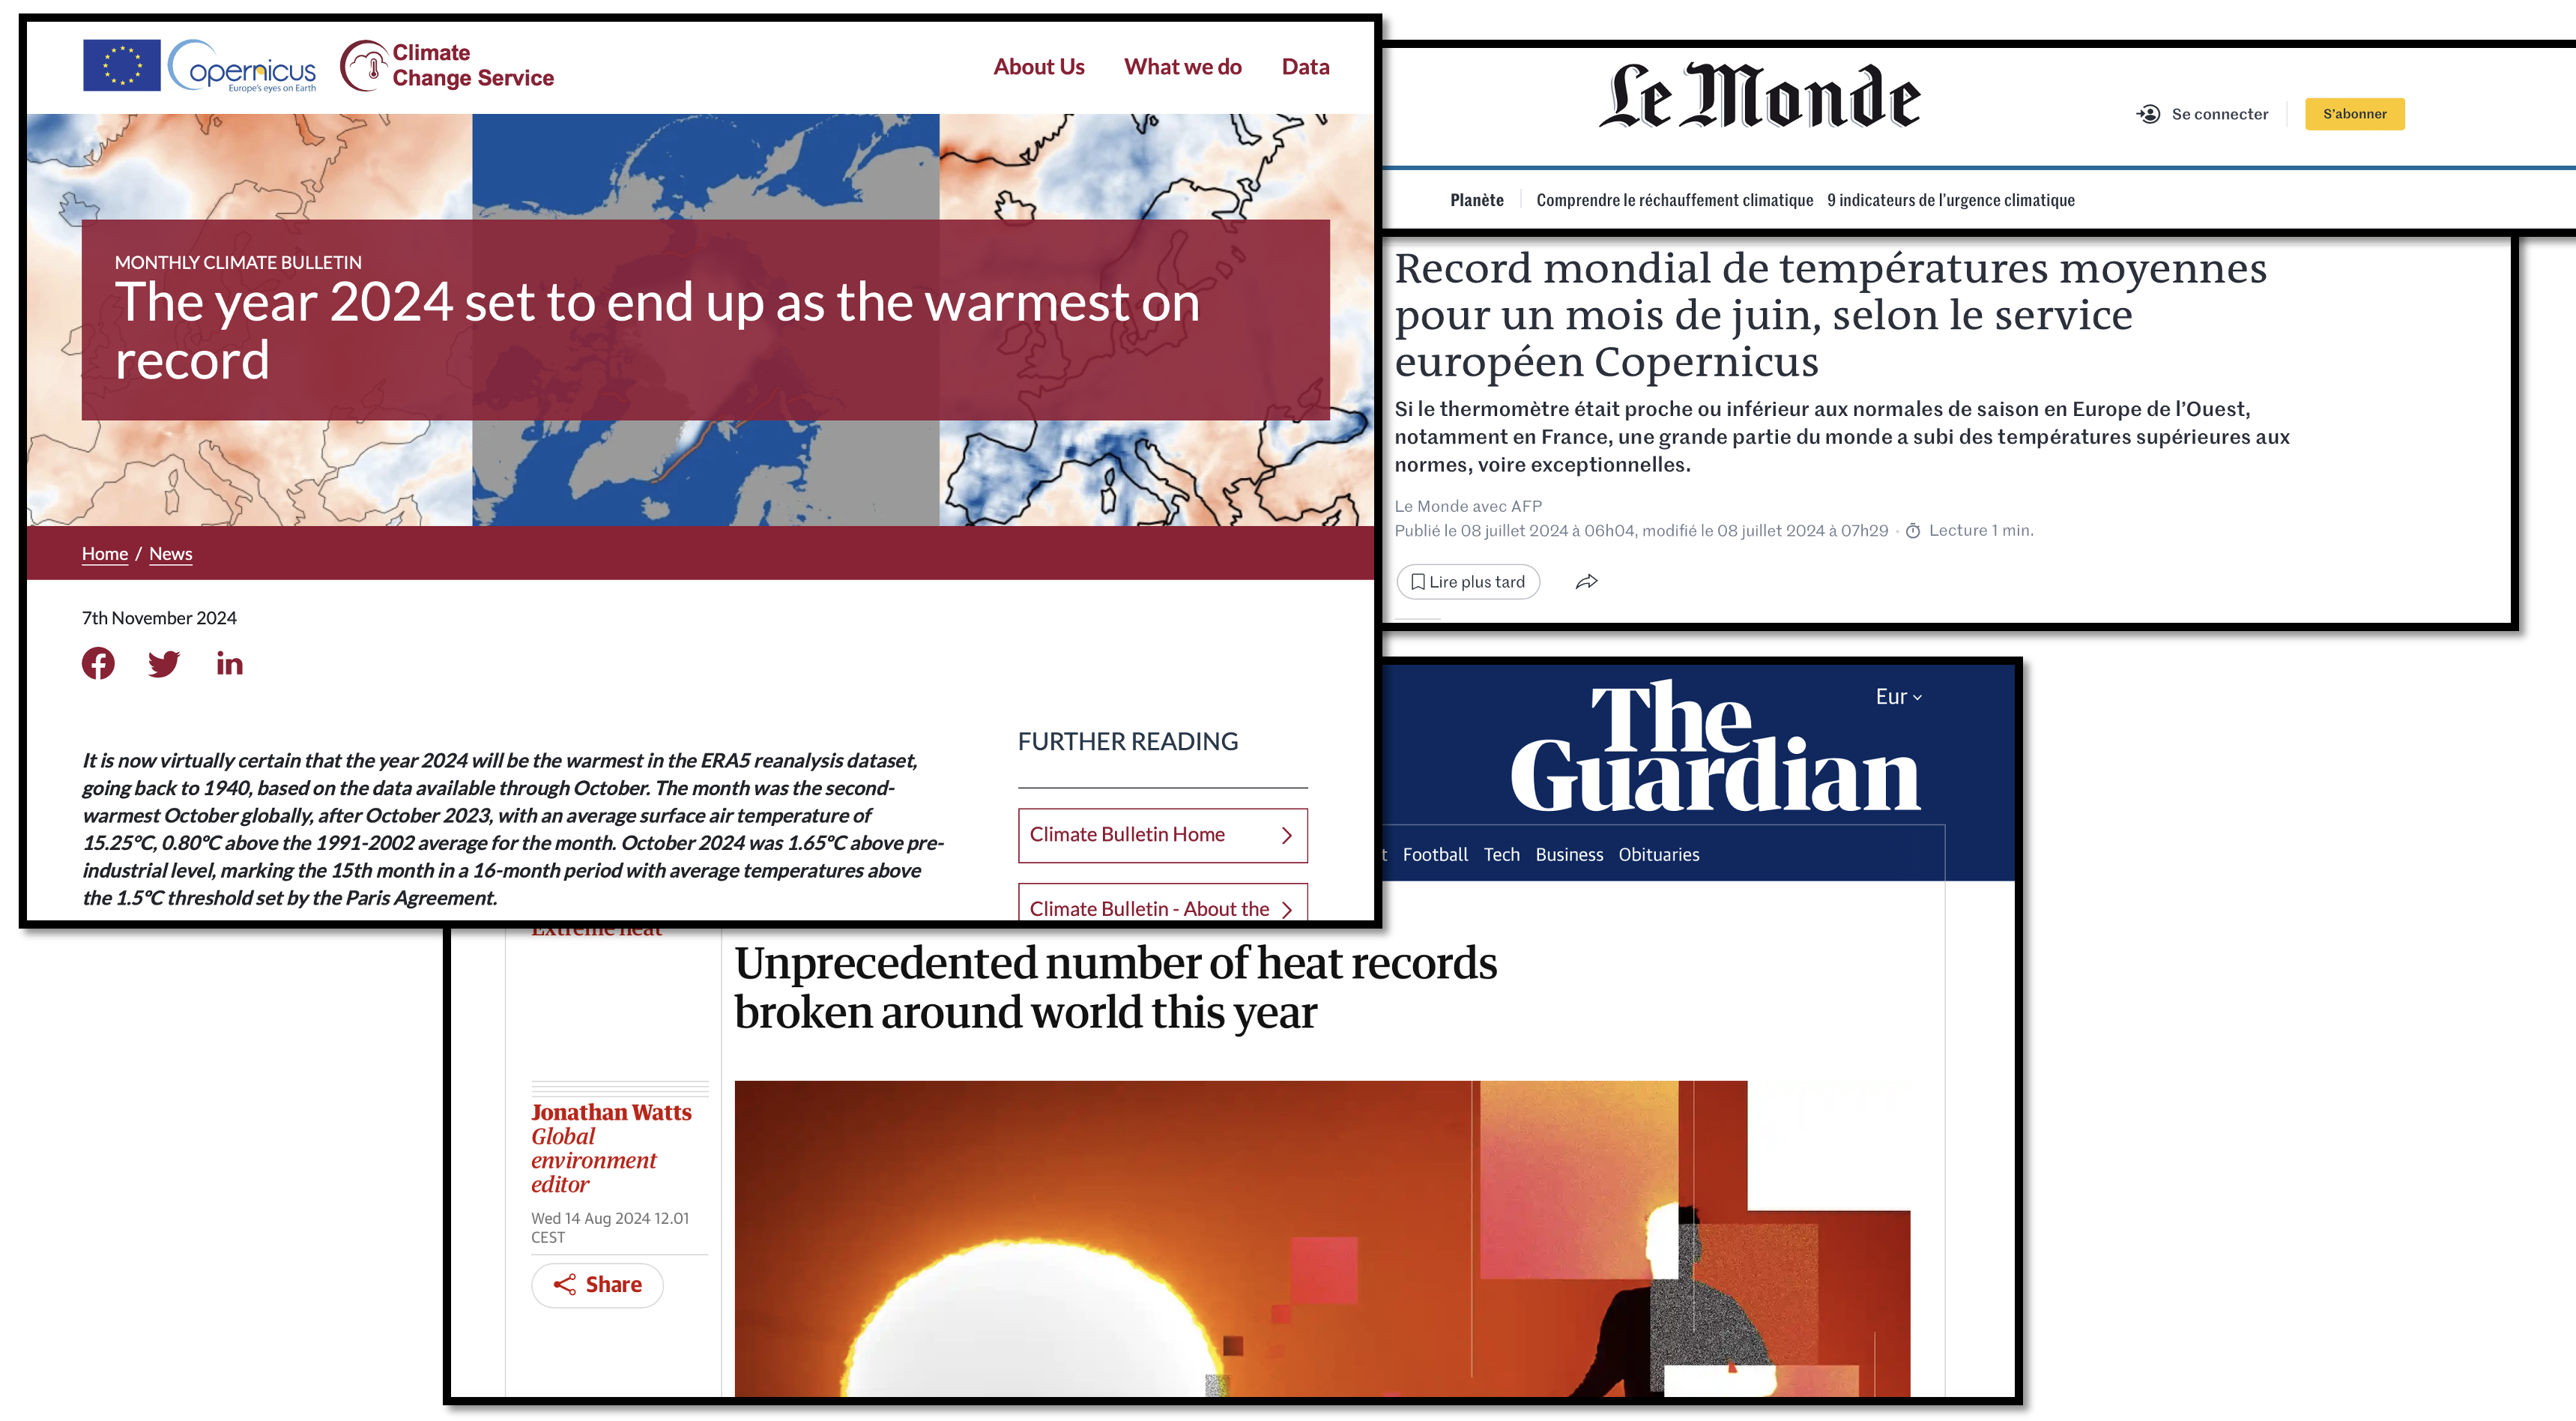
\includegraphics[width=1.12\textwidth]{/Users/pgonzale/Desktop/media_fig1_xaida.png} %\hfill
%\includegraphics[scale=0.37]{universe}\\
 %\end{center}    
\end{frame}
%%%%%%%%%%%%%%%%%%%%%%%%%%%%%%%%%%%%%% 
%
%
%
%%%%%%%%%%%%%%%%%%%%%%%%%%%%%%%%%%%%%%
%\begin{frame}
%\includegraphics[width=1\textwidth]{/Users/pgonzale/Desktop/ipccV2_figure_slide_soutenance.png} 
% \begin{center}
% {\color{beamer@blendedblue}\small ``Human-induced climate change is already affecting many weather and climate extremes in every region across the globe. Evidence of observed changes in extremes such as heatwaves, heavy precipitation, droughts, and tropical cyclones, and, in particular, their attribution to human influence, has strengthened since AR5''  (IPCC)} 
% \end{center}   
%\end{frame}
%%%%%%%%%%%%%%%%%%%%%%%%%%%%%%%%%%%%%% 
%
%
%
%%%%%%%%%%%%%%%%%%%%%%%%%%%%%%%%%%%%%% 
\begin{frame}{Records in Paris}
\only<2->{
\begin{tcolorbox}[title= What is a (high) record)$\; ^1$ ]
%$\{Y_t\} = \{Y_1,Y_2, \dots,Y_{T-1}\}$\\
%$\Re = \{1, 2\dots, T-1\}$
$$
%P_{T+1}(s_o) =P
\left\{  Y_{T}  > \max(Y_1, Y_2, \dots, Y_{T-1} )\right\}
$$
\end{tcolorbox}}\medskip

%\pause
\begin{figure}
\centering
    {\small\textbf{Yearly maxima of daily maxima temperature}}
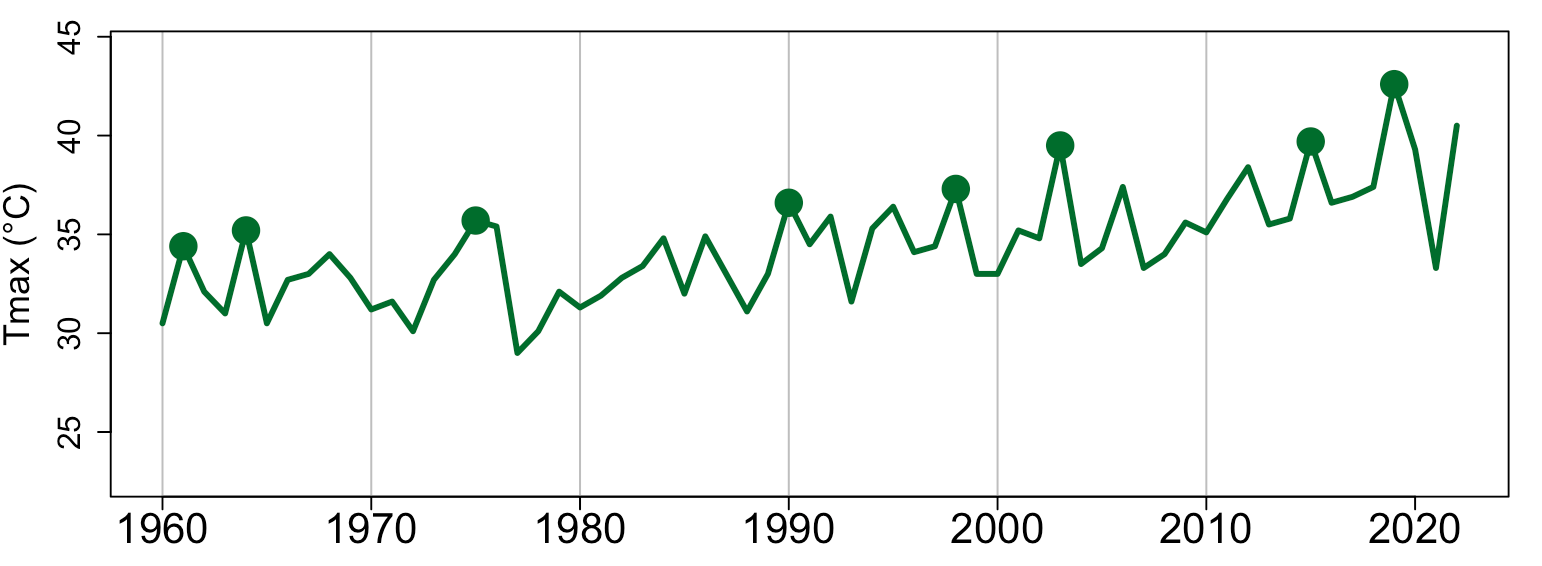
\includegraphics[scale=0.38]{/Users/pgonzale/Desktop/schema_1_xaida.png}\\
{\tiny Annual maxima of daily temperature maxima measured {at \color{red} Paris-Montsouris (Paris) station}  from 1960 to 2022}
\end{figure}
 \footnotetext[1]{\tiny  Chandler (1952) }
\end{frame}
%%%%%%%%%%%%%%%%%%%%%%%%%%%%%%%%%%%%%% 
%
%
%
%%%%%%%%%%%%%%%%%%%%%%%%%%%%%%%%%%%%%% 
\begin{frame}%{Records from yearly maxima of daily variables}
\begin{figure}
\centering
    {\small\textbf{Yearly maxima of daily maxima temperature}}
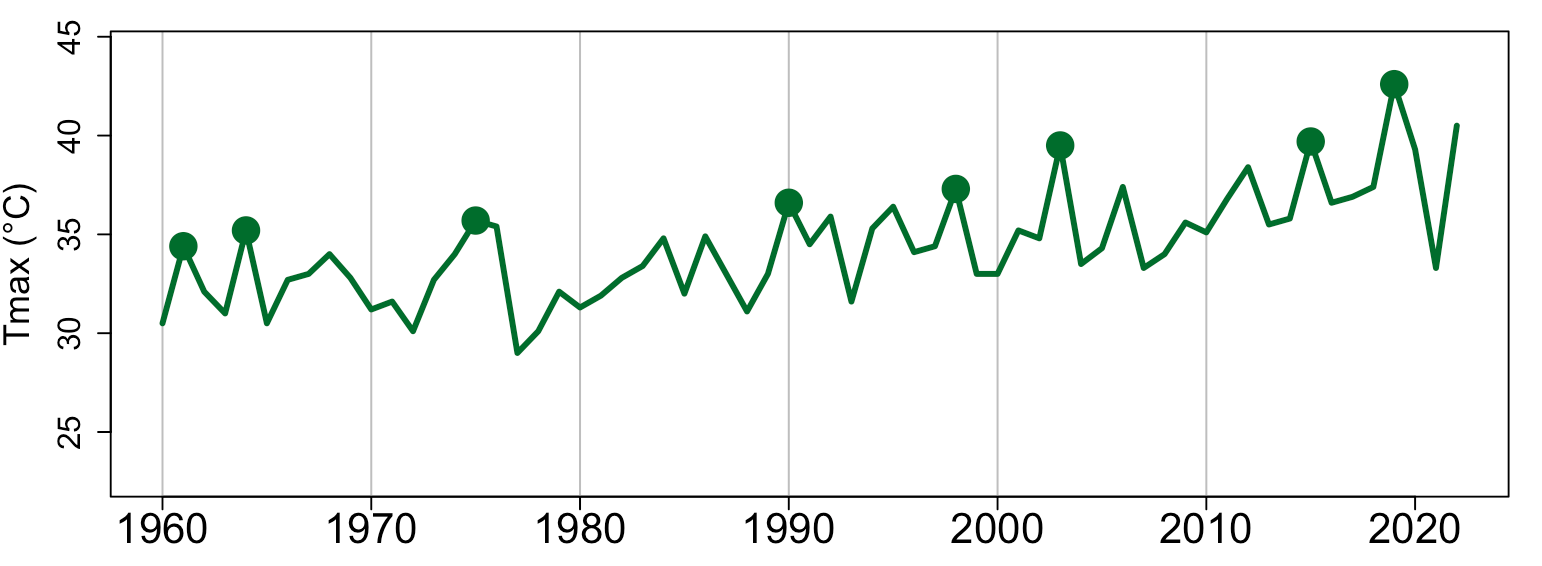
\includegraphics[scale=0.4]{/Users/pgonzale/Desktop/schema_1_xaida.png}\\
{\tiny Annual maxima of daily temperature maxima measured {at \color{red} Paris-Montsouris (Paris) station}  from 1960 to 2022}
\end{figure}

\begin{tcolorbox}[title= Questions of study]
 {\color{beamer@blendedblue}Q1 : }What are the odds, that a given year, e.g., 2030, could have beaten a 50-year counterfactual record?\\ 
 {\color{beamer@blendedblue}Q2 : } \pause What is the probability of observing a record in 2023 in the center of Paris given measurement around Paris recorded up to 2022?
\end{tcolorbox}

\end{frame}
%%%%%%%%%%%%%%%%%%%%%%%%%%%%%%%%%%%%%% 
%
%
%
\setbeamercolor{section in head/foot}{bg=gray@schema}
\setbeamercolor{subsection in head/foot}{bg=gray@schema}
%%%%%%%%%%%%%%%%%%%%%%%%%%%%%%%%%%%%%% 
\section{Summary of problematics}
\begin{frame}{Q1 : What are the odds, that a given year, e.g., 2030, could have beaten a 50-year counterfactual record? }
\begin{center}
%\includegraphics[width=0.5\textwidth]{/Users/pgonzale/Desktop/yellowpart_intro_slide.png}
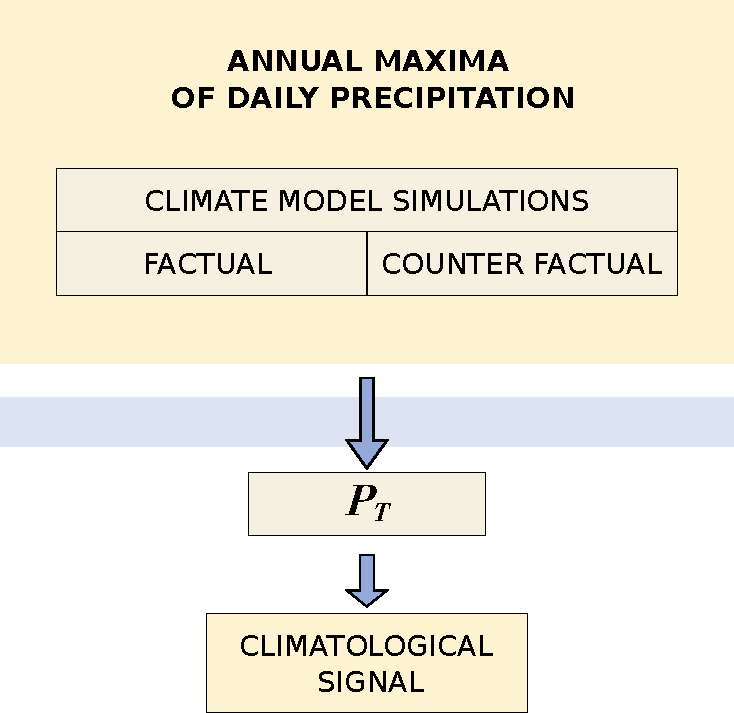
\includegraphics[width=0.6\textwidth]{/Users/pgonzale/Downloads/yellow_intro.pdf}
 \end{center}    
 \pause
     \begin{tikzpicture}[remember picture, overlay,use page relative coordinates]
  \node[anchor=north east] at (1.024,0.53) {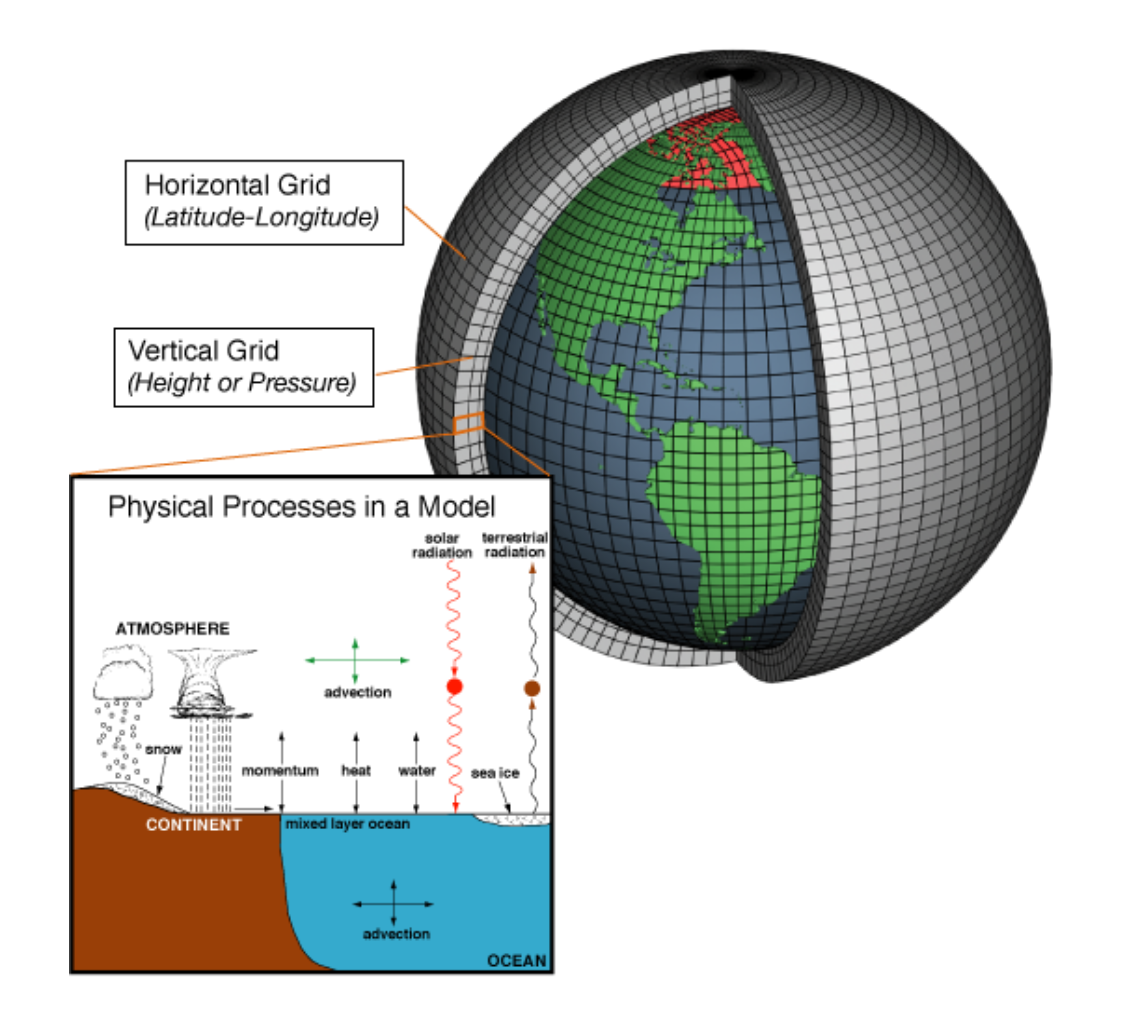
\includegraphics[width=0.44\textwidth]{/Users/pgonzale/Desktop/climate_models_representation.png}};

  \end{tikzpicture}


\end{frame}
%%%%%%%%%%%%%%%%%%%%%%%%%%%%%%%%%%%%%% 
%
%
%
%%%%%%%%%%%%%%%%%%%%%%%%%%%%%%%%%%%%%% 
\section{Summary of problematics} 
\begin{frame}{Q2 : What is the probability of observing a record in 2023 in the center of Paris given measurement around Paris recorded up to 2022?}
\begin{center}
%\includegraphics[width=0.5\textwidth]{/Users/pgonzale/Desktop/redpart_intro_slide.png}
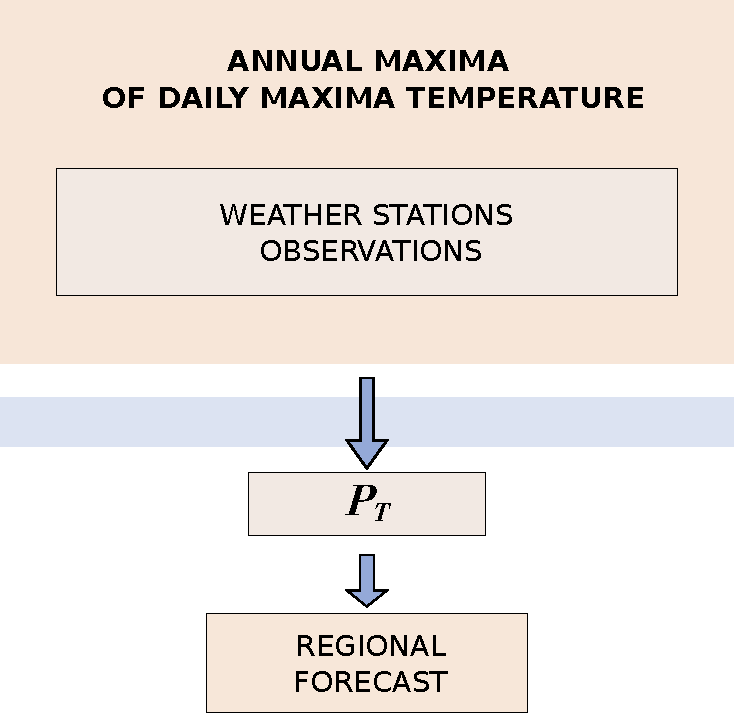
\includegraphics[width=0.6\textwidth]{/Users/pgonzale/Downloads/red_intro.pdf}
 \end{center}    
  \pause
     \begin{tikzpicture}[remember picture, overlay,use page relative coordinates]
  \node[anchor=north east] at (1.02,0.53) {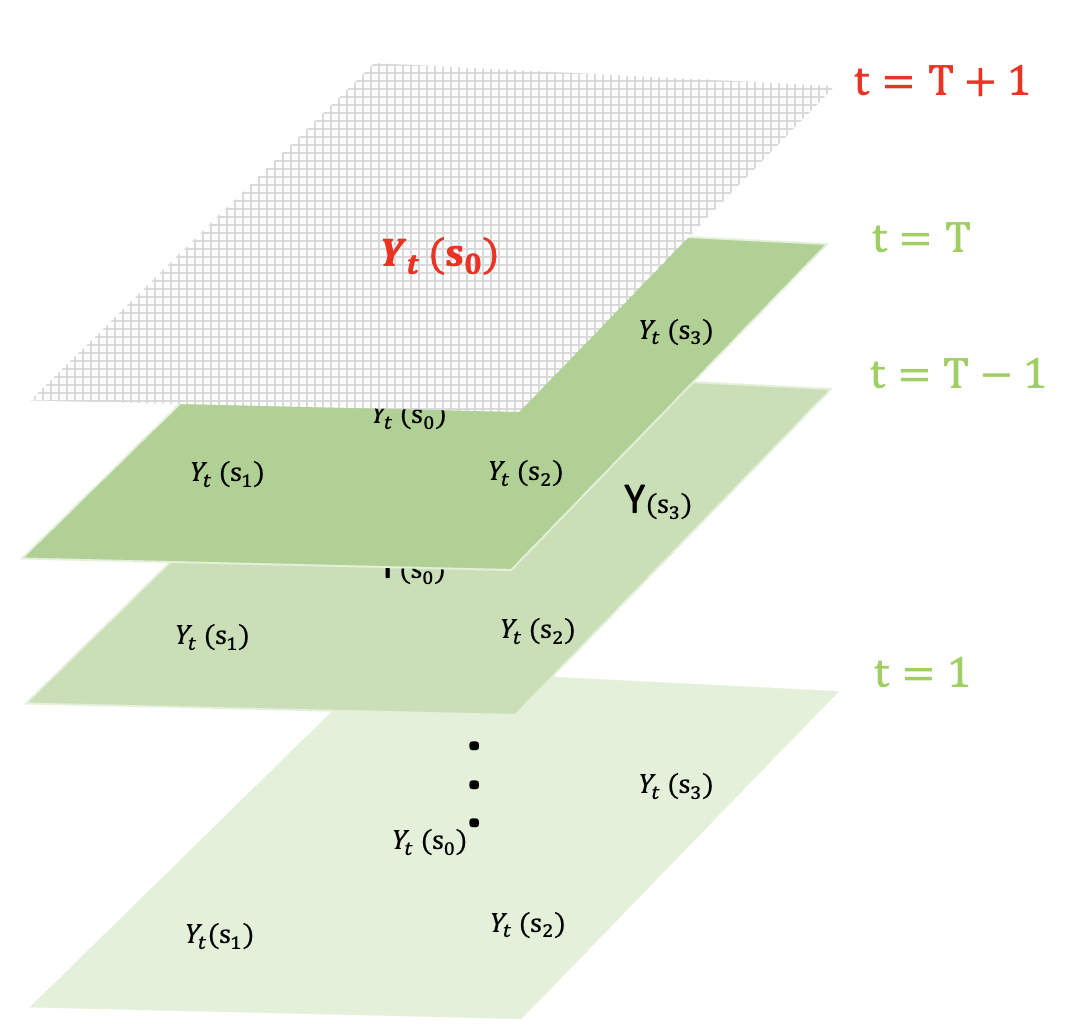
\includegraphics[width=0.43\textwidth]{/Users/pgonzale/Desktop/schema_Q2_surfaces.png}};

  \end{tikzpicture}
\end{frame}
%%%%%%%%%%%%%%%%%%%%%%%%%%%%%%%%%%%%%% 
%
%
%
%%%%%%%%%%%%%%%%%%%%%%%%%%%%%%%%%%%%%% 
\section{Summary of problematics} 
\begin{frame} 
\begin{center}
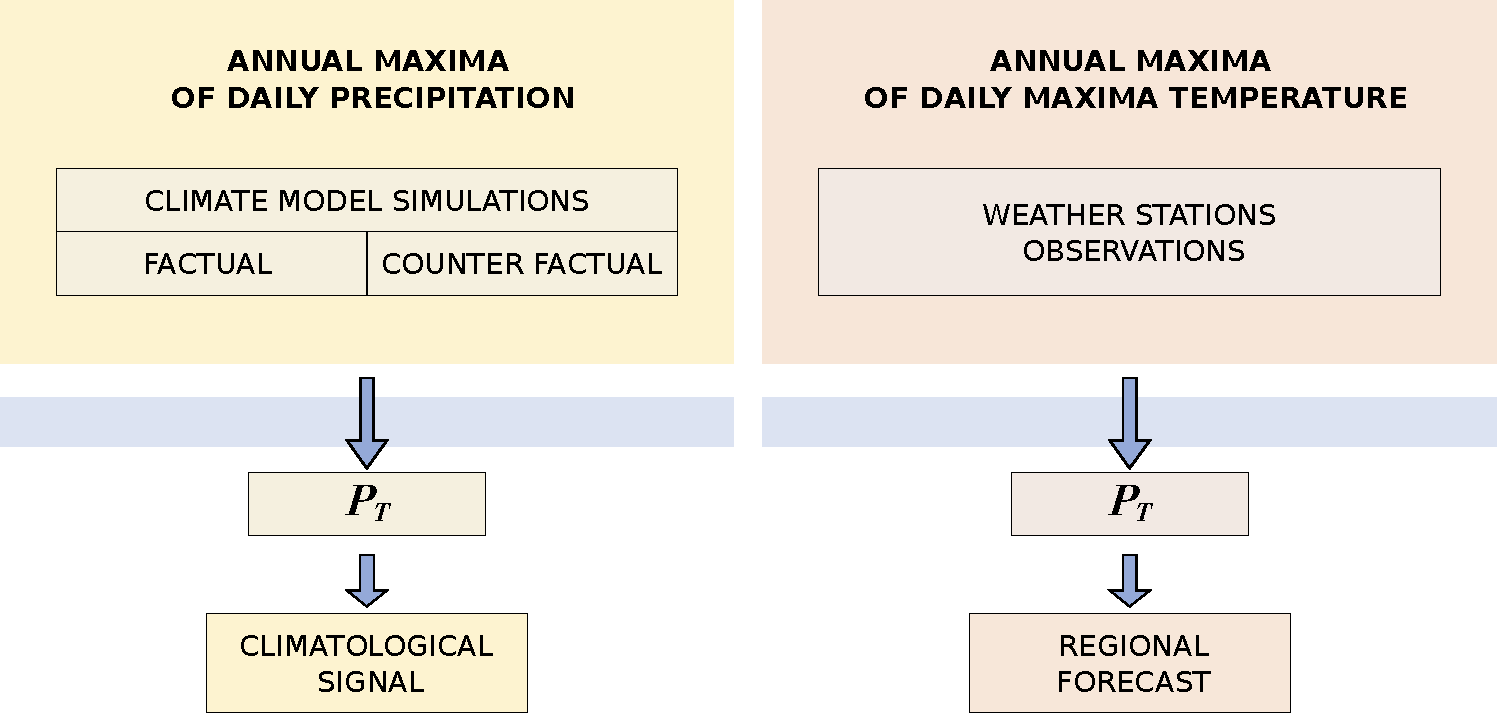
\includegraphics[width=1\textwidth]{/Users/pgonzale/Downloads/yellow_red_intro.pdf}
\end{center}
\end{frame}
%%%%%%%%%%%%%%%%%%%%%%%%%%%%%%%%%%%%%% 
%
%
%
%%%%%%%%%%%%%%%%%%%%%%%%%%%%%%%%%%%%%% 
\begin{frame}%{Surface temperatures records}
\begin{tcolorbox}[title= Limitations that we need to address]
\begin{itemize}
	\item Statistical modeling of record probability from yearly maxima and its evolution through time. 
	\item Inference of a climate signal on record probability at a specific location.
	\item Incorporation of spatial information through the proper modeling of the dependencies among time series.
\end{itemize}
\end{tcolorbox}
\end{frame}
%%%%%%%%%%%%%%%%%%%%%%%%%%%%%%%%%%%%%% 
%
%
%
\setbeamercolor{section in head/foot}{bg=blue@schema}
\setbeamercolor{subsection in head/foot}{bg=blue@schema}
%%%%%%%%%%%%%%%%%%%%%%%%%%%%%%%%%%%%%% 
\section{Background}
\begin{frame}{Q1 : What are the odds, that a given year, e.g., 2030, could have beaten a 50-year counterfactual record?}
\begin{center}
%\includegraphics[width=0.36\textwidth]{/Users/pgonzale/Desktop/yellowpart_complete_slide.png}
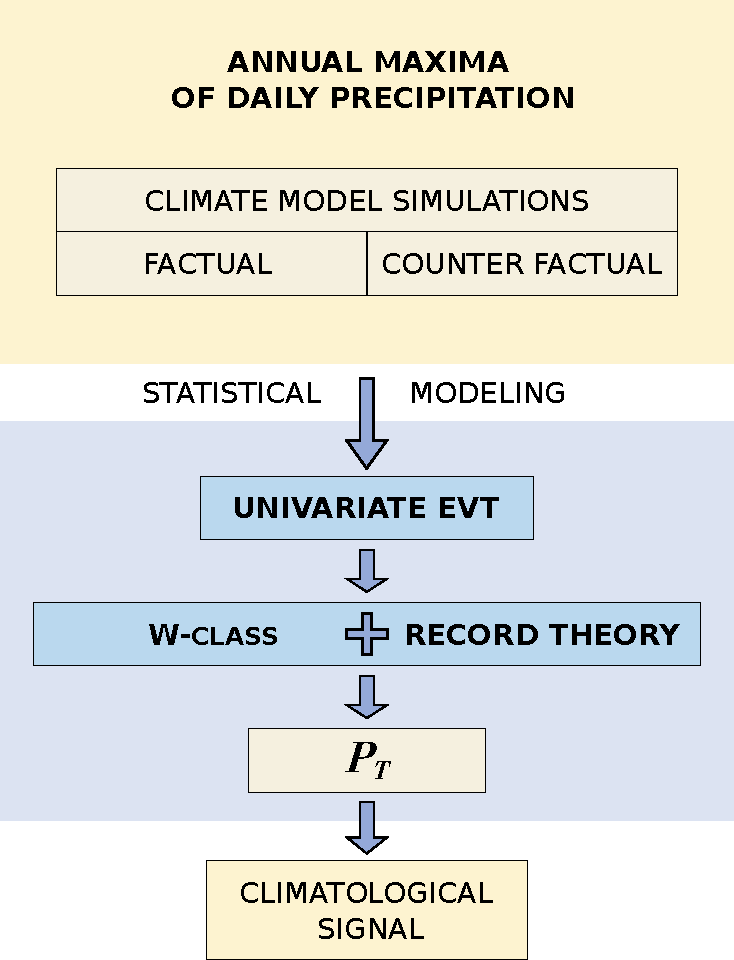
\includegraphics[width=0.5\textwidth]{/Users/pgonzale/Downloads/yellow_model.pdf}
 \end{center}    
\end{frame}
%%%%%%%%%%%%%%%%%%%%%%%%%%%%%%%%%%%%%% 
%
%
%
%%%%%%%%%%%%%%%%%%%%%%%%%%%%%%%%%%%%%% 
\begin{frame}{Extreme value theory for annual maxima \footnotemark[2]}  %\footnotemark[1]

\begin{tcolorbox}[title= Annual maxima distribution ]
$M_n=\max \{X_1,\dots,X_n\}$ of $n$ i.i.d. R.V\\
  $$
   (M_n - b_n)/a_n \xrightarrow[]{d}
GEV({\color{beamer@blendedblue}\mu},{\color{beamer@blendedblue}\sigma}, {\color{beamer@blendedblue}\xi})\quad \text{when}\quad n \xrightarrow[]{} \infty
$$
\end{tcolorbox}
\pause
%\hfill
%\begin{itemize}
%\item $\xi > 0$ : heavy-tailed GEV distribution of support $(\mu-\sigma/\xi,\infty)$.\\ {\tiny(Fréchet)}
%\item $\xi = 0$ : GEV distribution of support $(-\infty,\infty)$. \\{\tiny(Gumbel)}
%\item $\xi < 0$ : light-tailed GEV distribution of support $(-\infty,\mu-\sigma/\xi)$. \\{\tiny(Weibull)}
%\end{itemize}
\begin{columns}
\begin{column}{0.45\textwidth}
%\begin{center}
\begin{itemize}
\centering
\item ${\color{blue}\xi > 0}$\\ {\tiny e.g. Yearly maxima of daily precipitation \footnotemark[3]}\bigskip

 %: heavy-tailed GEV distribution of support $(\mu-\sigma/\xi,\infty)$.\\ {\tiny(Fréchet)}
\item ${\color{red}\xi = 0}$\bigskip

 %: GEV distribution of support $(-\infty,\infty)$. \\{\tiny(Gumbel)}
\item ${\color{green}\xi < 0}$\\ {\tiny e.g. Yearly maxima of daily maxima temperature \footnotemark[3]}\\
 %: light-tailed GEV distribution of support $(-\infty,\mu-\sigma/\xi)$. \\{\tiny(Weibull)}
\end{itemize}
%\end{center}
\end{column}
\begin{column}{0.55\textwidth}
%\begin{center}
 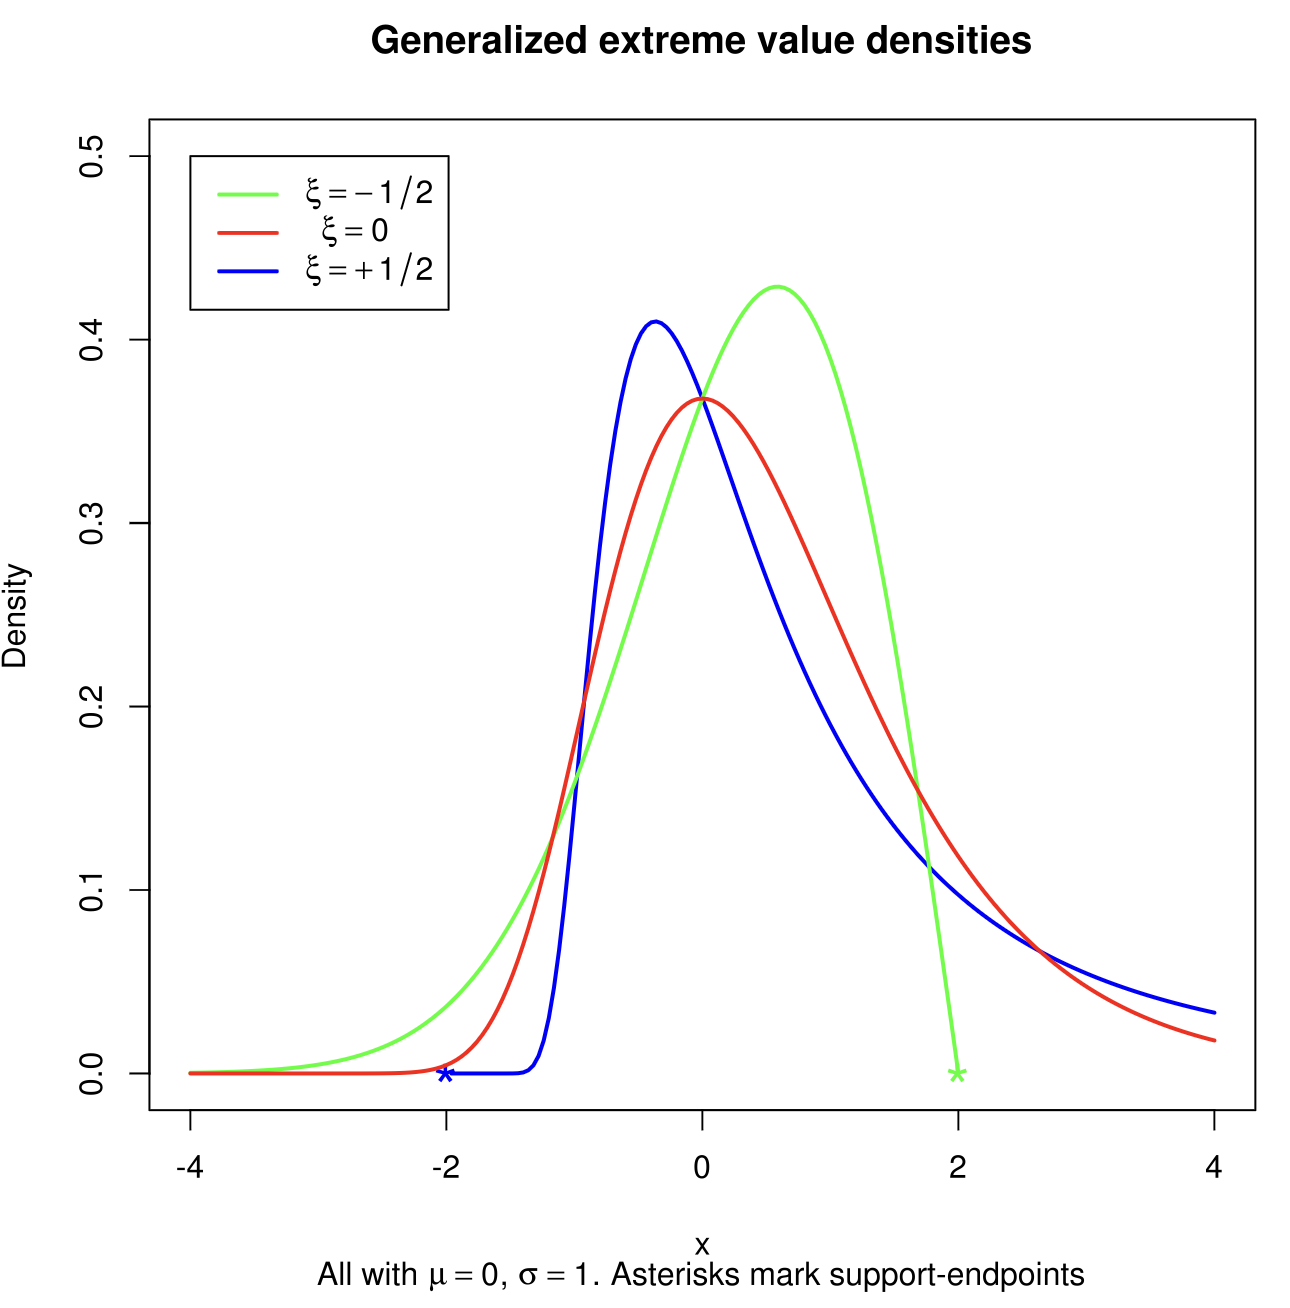
\includegraphics[scale=0.22]{/Users/pgonzale/Desktop/gev_wikipedia_slides_soutenance.png}
%\end{center}
\end{column}
\end{columns}
\vfill
%       {\it \tiny see, e.g.  Statistics of Extremes, 
%Davison and Huser
%Annual Review of Statistics and Its Application 2015 2:1, 203-235 }  
    %\footnotetext[1]{Coles (2001); Beirlant et al. (2004)} 
    \footnotetext[2]{ \tiny see, e.g.  Statistics of Extremes, 
Davison and Huser
Annual Review of Statistics and Its Application 2015 2:1, 203-235}
 \footnotetext[3]{\tiny Cooley et al. (2007), Kharin and Zwiers (2005)}
 % \footnotetext[3]{\tiny Kharin and Zwiers (2005)} 
\end{frame}
%%%%%%%%%%%%%%%%%%%%%%%%%%%%%%%%%%%%%% 
%
%
%
%%%%%%%%%%%%%%%%%%%%%%%%%%%%%%%%%%%%%% 
 \begin{frame}{W-class}   

\begin{tcolorbox}[title= Characterizing records by the relative behavior$\; ^4$]
$Z \,\bot\, X$ random variables with  $G(x) = P(X\leq x) $
$$
P(Z>\max\{X_1,X_2,\dots, X_r\}) = \mathbb{E}(exp(-r{\color{beamer@blendedblue}W})).
$$
$$\text{with}\quad  {\color{beamer@blendedblue}W=-\log G(Z)}$$
\end{tcolorbox}
\pause

\begin{tcolorbox}[title=Definition (W-class)$\; ^5$]]
Let $X\sim G$ and $Z\sim F$ be two random variables with the same support. We say that {\color{beamer@blendedblue}the couple $(X,Z)$ belongs to the $W$-class} if the random variables $W=-\log G(Z)$ is {\color{beamer@blendedblue}Weibull} distributed with parameters {\color{beamer@blendedblue} $(k,\lambda)$}, i.e,
$$ P(W>w) = \exp (-(w/\lambda)^{k})\quad \text{for any}\quad w> 0$$
\end{tcolorbox}
\footnotetext[4]{\tiny Naveau et al. (2018)}
\footnotetext[5]{\tiny Worms and Naveau (2022)}
\end{frame}
%%%%%%%%%%%%%%%%%%%%%%%%%%%%%%%%%%%%%% 
%
%
%
%%%%%%%%%%%%%%%%%%%%%%%%%%%%%%%%%%%%%% 
\section{Background}
\begin{frame}{Q2 : What is the probability of observing a record in 2023 in the center of Paris given measurement around Paris recorded up to 2022?}
\begin{center}
%\includegraphics[width=0.36\textwidth]{/Users/pgonzale/Desktop/redpart_complete_slide.png}
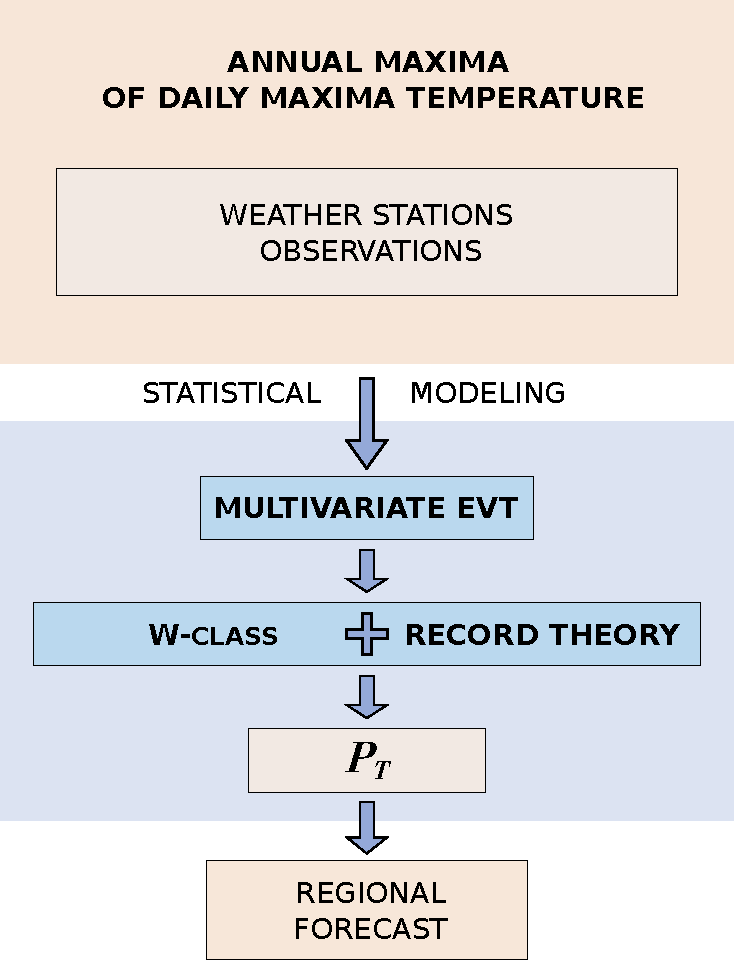
\includegraphics[width=0.5\textwidth]{/Users/pgonzale/Downloads/red_model.pdf}
 \end{center}    
\end{frame}
%%%%%%%%%%%%%%%%%%%%%%%%%%%%%%%%%%%%%% 
%
%
%
%%%%%%%%%%%%%%%%%%%%%%%%%%%%%%%%%%%%%% 
 \begin{frame}{EVT for componentwise maxima\footnotemark[6] }   
If we consider the componentewise maximum ${\bf M}_n=\left(M_{n;1},\dots,M_{n;d}\right)^T$ of $n$ i.i.d. d-dimensional random vectors ${\bf X}$
\begin{tcolorbox}[title= Multivariate block maxima distribution (with unit-Fr\'echet marginals)]
  $$
   \frac{{\bf M}_n - b_n}{a_n} \xrightarrow[]{d}
MGEV( {\bf x}) ={\color{beamer@blendedblue}\exp \left\{ - V( {\bf x} )\right\}} \quad \text{when}\quad n \xrightarrow[]{} \infty
$$
\begin{center}
with ${\bf x}=(x_1, \dots, x_d)^T$ and \\${\color{beamer@blendedblue}V({\bf x})}$ a positive homogenous function of order -1, i.e. ${\color{beamer@blendedblue}V( {c\bf x} )=c^{-1}V( {\bf x} )}$ 
\end{center}
\end{tcolorbox}
       %{\it \tiny see, e.g.  Fougères (2004),  SpatialExtremes package (R)}  
       \footnotetext[6]{\it \tiny see, e.g.  Fougères (2004),  SpatialExtremes package (R)}
\end{frame}
%%%%%%%%%%%%%%%%%%%%%%%%%%%%%%%%%%%%%% 
%
%
%
%%%%%%%%%%%%%%%%%%%%%%%%%%%%%%%%%%%%%% 
\begin{frame}%{Surface temperatures records}
\begin{center}
\vspace{0.7cm}
%\includegraphics[width=0.75\textwidth]{/Users/pgonzale/Desktop/redandyellow_complete_slide.png}
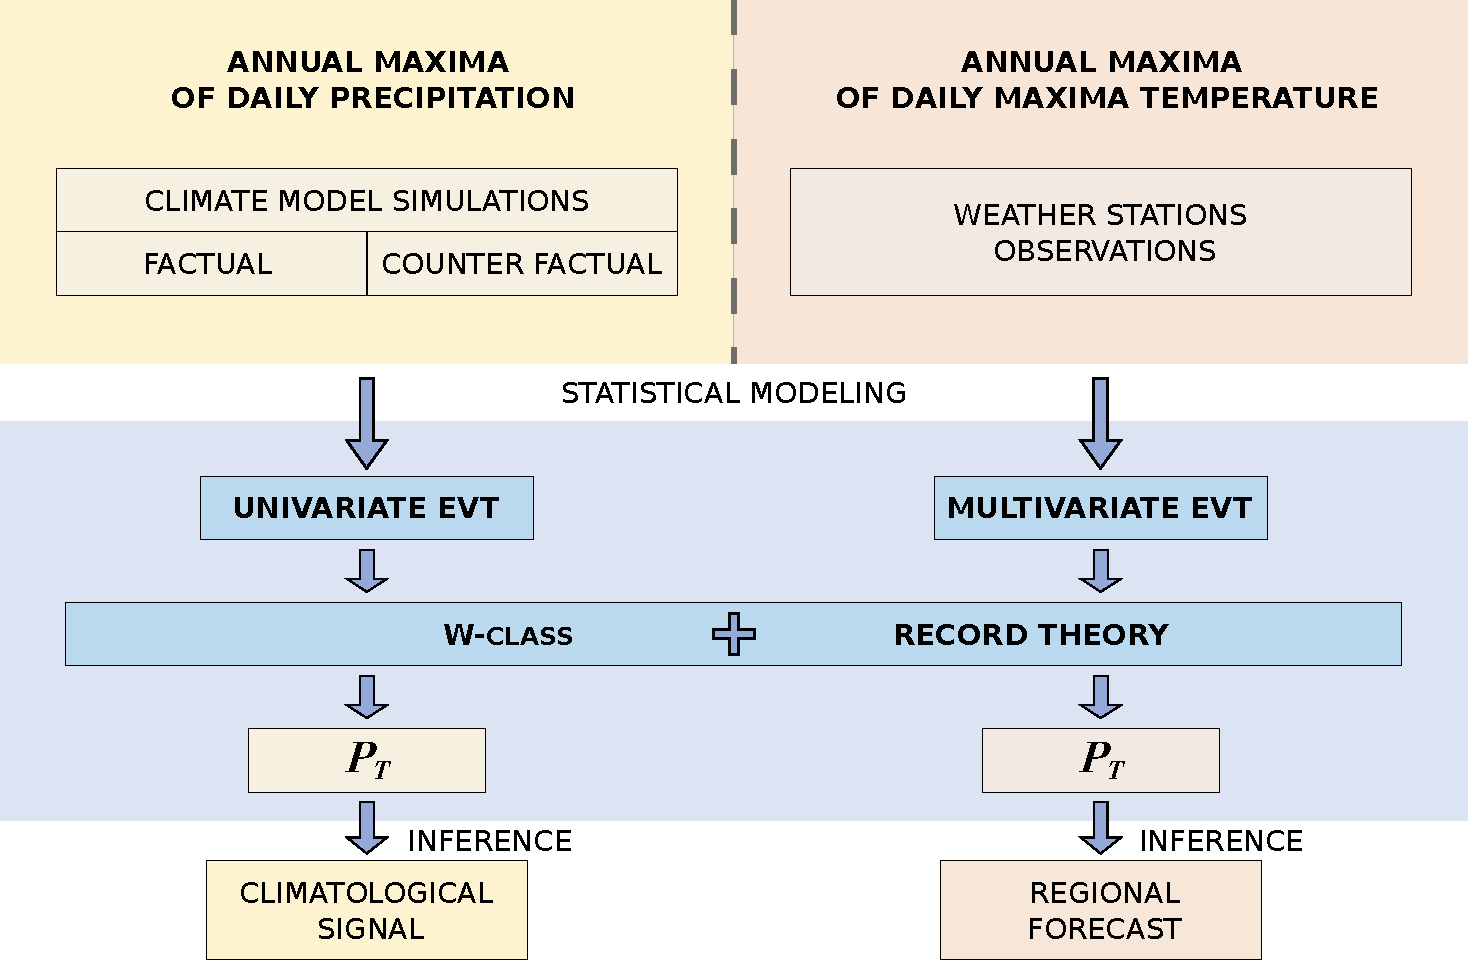
\includegraphics[width=1\textwidth]{/Users/pgonzale/Downloads/yellow_red_model.pdf}
 \end{center}
 
   \begin{tikzpicture}[remember picture, overlay,use page relative coordinates]
  %Q1 : What are the odds, that a given year, e.g., 2030, could have beaten a 50-year counterfactual record? 
  %\node[anchor=north west] at (0,1) {(0,1)};
  \node[anchor=north west] at (0.04,0.95) {{\color{beamer@blendedblue}\tiny Q1 : What are the odds, that a given year, e.g., 2030,}};
   \node[anchor=north west] at (0.075,0.93) {{\color{beamer@blendedblue}\tiny could have beaten a 50-year counterfactual record?}};
    %\node[anchor=north west] at (0.075,0.928) {{\color{beamer@blendedblue}\tiny recorded up to 2022?}};
    
  % showing a couple of example coordinates
  %\node[anchor=south west] at (0,0) {(0,0)};
  %\node[anchor=south east] at (1,0) {(1,0)};
  %\node[anchor=north west] at (0,1) {(0,1)};
  \node[anchor=north east] at (0.98,0.97) {{\color{beamer@blendedblue}\tiny Q2 : What is the probability of observing a record in 2023}};
   \node[anchor=north east] at (0.99,0.95) {{\color{beamer@blendedblue}\tiny in the center of Paris given measurement around Paris}};
    \node[anchor=north east] at (0.787,0.93) {{\color{beamer@blendedblue}\tiny recorded up to 2022?}};
   %\node at (0.7,0.3) {test}; 
    
  \end{tikzpicture}
      
\end{frame}
%%%%%%%%%%%%%%%%%%%%%%%%%%%%%%%%%%%%%% 
%
%
%
\setbeamercolor{section in head/foot}{bg=yellow@schema}
\setbeamercolor{subsection in head/foot}{bg=yellow@schema}
%%%%%%%%%%%%%%%%%%%%%%%%%%%%%%%%%%%%%% 
\section{Part 1}
{\setbeamercolor{background canvas}{bg=yellow@schema}
\begin{frame}
\begin{center}
\textbf{\LARGE {\color{beamer@blendedblue} A statistical method to model non-stationarity\\
 in precipitation records changes}}
 \bigskip
 \bigskip

\LARGE {\color{beamer@blendedblue} (Part 1)}
\end{center}
 \bigskip
 \bigskip
 \bigskip
 \bigskip
 
{\tiny
\begin{myboxyellow}
Accepted in Geophysical Research Letters (Gonzalez et al., 2024).
\end{myboxyellow}
}
\end{frame}




}
%%%%%%%%%%%%%%%%%%%%%%%%%%%%%%%%%%%%%% 
%
%
%
%%%%%%%%%%%%%%%%%%%%%%%%%%%%%%%%%%%%%% 
\begin{frame}{Preamble on Extreme Event Attribution (EEA) \footnotemark[7] }
\begin{columns}
\begin{column}{0.5\textwidth}
\begin{center}
\includegraphics[scale=0.2]{/Users/pgonzale/Desktop/chap2_preamble_1.png}
Counterfactual \footnotemark[8] {\color{blue} $X$}\\ 
Factual  {\color{red} $Z$}  
 \end{center}  
 \end{column}
 \pause
 \begin{column}{0.5\textwidth}
\begin{center}
\only<3->{\includegraphics[scale=0.4]{/Users/pgonzale/Desktop/Berta/chap2_intro_EEA_F_CF.png}}
${\color{blue} p_0}=P({\color{blue}X}>u)$\\ 
${\color{red} p_1}=P({\color{red}Z}>u)$\\ 
 \end{center}    
 \end{column}
 \end{columns}
  \footnotetext[7]{\tiny Scott et al.(2016); Allen (2003) }
 \footnotetext[8]{\tiny Hannart et al. (2016), Angélil et al. (2017), Hegerl and Zwiers (2011)}
\end{frame}
%%%%%%%%%%%%%%%%%%%%%%%%%%%%%%%%%%%%%%
%
%
%
%%%%%%%%%%%%%%%%%%%%%%%%%%%%%%%%%%%%%% 
\begin{frame}%{EEA of records}
\begin{tcolorbox}[title= Literature on EEA for records ]
	\begin{itemize}
			\item EEA of records based on counting record occurrences, e.g King (2017) %detection and emergence of forced change
			\item Statistical models in a stationary framework, e.g {\bf \color{beamer@blendedblue} Worms and Naveau (2022)}, Naveau et al. (2018)
			% records have usually been studied in a stationary context, with limited advances on non-stationary times series.
			\item Very sparse for non-stationary times series.
\end{itemize}
\end{tcolorbox}
\end{frame}
%%%%%%%%%%%%%%%%%%%%%%%%%%%%%%%%%%%%%%  
%
%
%
%%%%%%%%%%%%%%%%%%%%%%%%%%%%%%%%%%%%%% 
\begin{frame}{Q1}
%\LARGE {\color{beamer@blendedblue} \bf Q1 :}\\
\begin{center}
\LARGE {\color{beamer@blendedblue} What are the odds that a given year, e.g 2050, could have beaten a r-year counterfactual record?}
\end{center}
%\pause
\vfill
e.g. $r= 50$
\end{frame}
%%%%%%%%%%%%%%%%%%%%%%%%%%%%%%%%%%%%%% 
%
%
%
%%%%%%%%%%%%%%%%%%%%%%%%%%%%%%%%%%%%%% 
\begin{frame}{EEA of records}
\begin{tcolorbox}[title= Question ]
What are the odds that a given year, e.g 2050, could have beaten a r-year counterfactual record?
\end{tcolorbox}
\begin{tcolorbox}[title= Event of interest : beat a r-year counterfactual record ]
being larger that the maxima of the $r-1$ previous {\color{blue}counterfactual} realizations
\end{tcolorbox}
\pause
\begin{tcolorbox}[title= Mathematical definition ]
$${\color{blue}p_{0,r}(t)} = P({\color{blue}X_t}> \max (X_{t-1},\dots, X_{t-r+1}))$$ 
$${\color{red}p_{1,r}(t)} = P({\color{red}Z_t}> \max (X_{t-1},\dots, X_{t-r+1}))$$ 
\end{tcolorbox}
\end{frame}
%%%%%%%%%%%%%%%%%%%%%%%%%%%%%%%%%%%%%% 
%
%
%
%%%%%%%%%%%%%%%%%%%%%%%%%%%%%%%%%%%%%% 
\begin{frame}{EEA of records}
\begin{tcolorbox}[title= Question ]
What are the odds that a given year, e.g 2050, could have beaten a r-year counterfactual record?
\end{tcolorbox}

%\pause
\begin{figure}
\centering
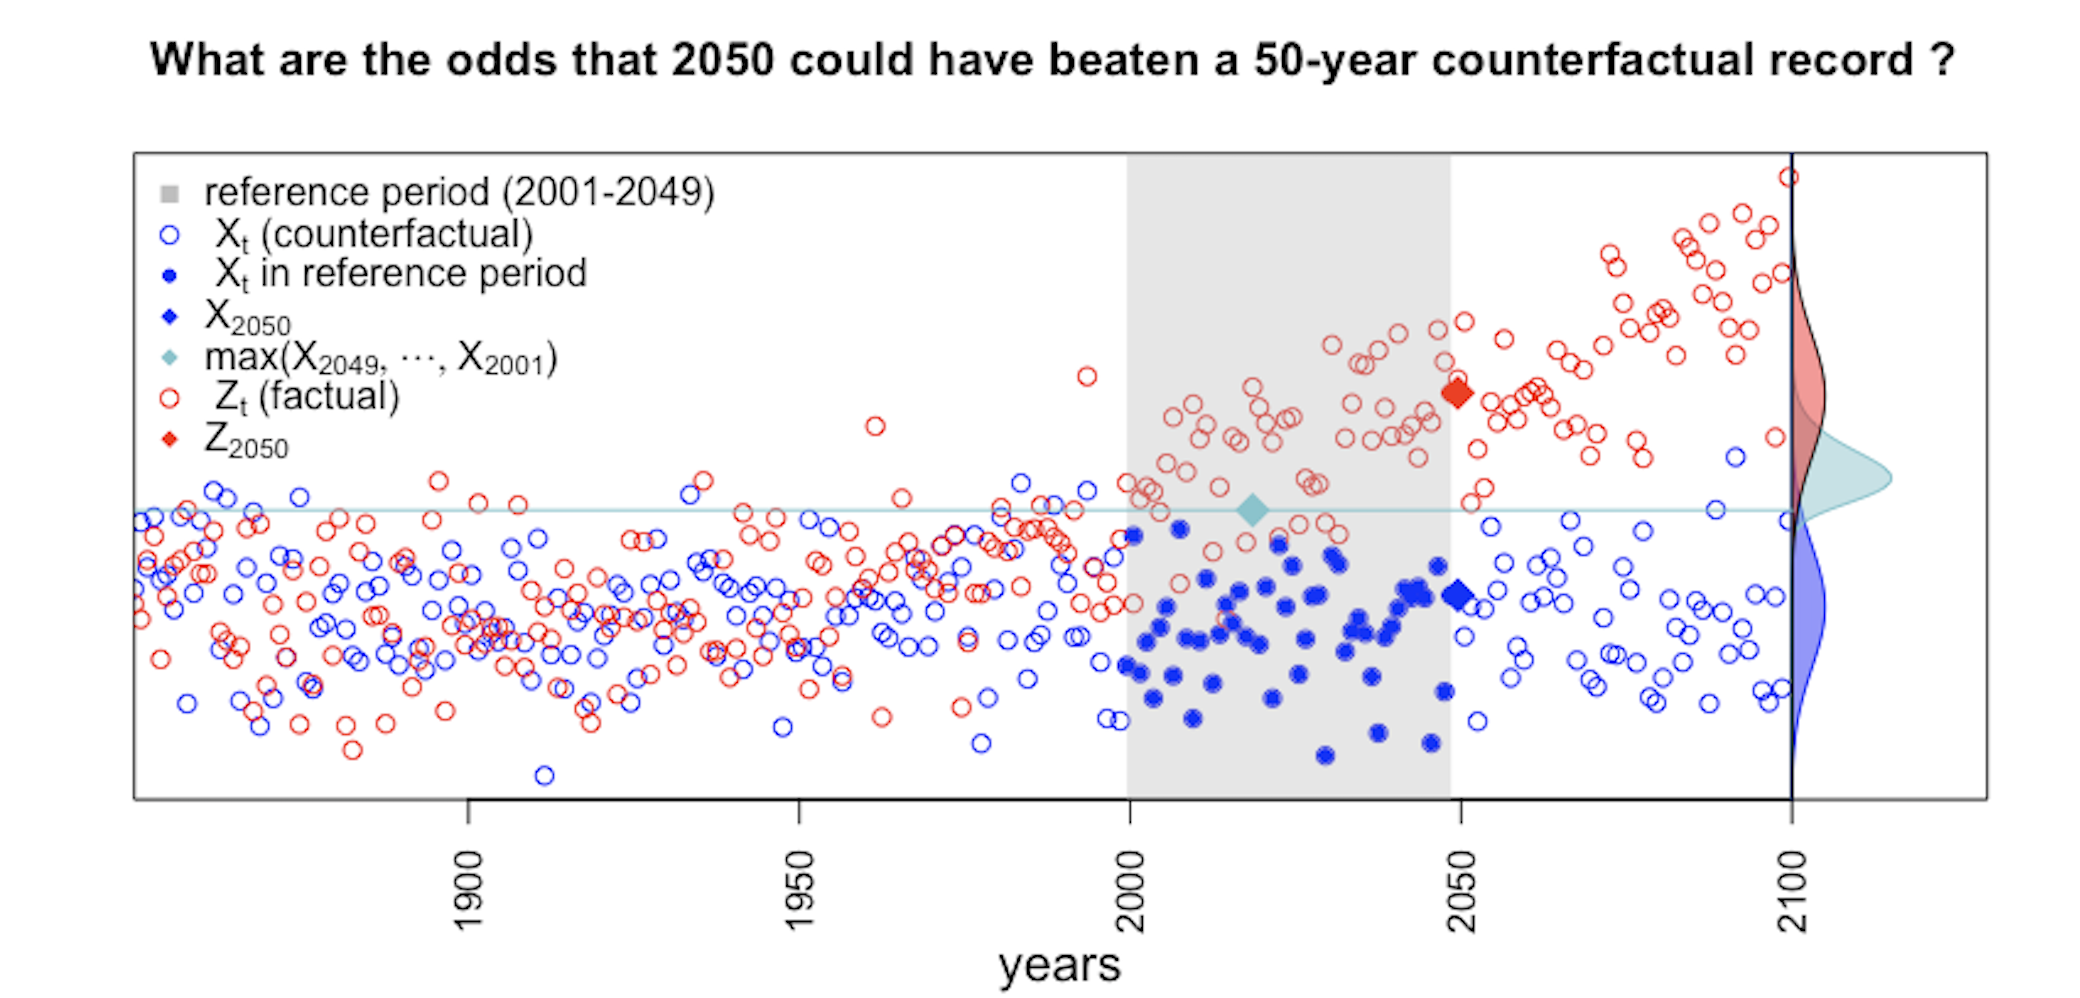
\includegraphics[width=1\textwidth]{/Users/pgonzale/Desktop/Berta/fig2_JDD.png}
\end{figure}
\end{frame}
%%%%%%%%%%%%%%%%%%%%%%%%%%%%%%%%%%%%%% 
%
%
%
%%%%%%%%%%%%%%%%%%%%%%%%%%%%%%%%%%%%%% 
\begin{frame}{Record probability in a stationary climate \footnotemark[9]}
\begin{tcolorbox}[title= Record probability in the counterfactual world ]
$X_{r-1}, \dots, X_1$ are exchangeable 
$${\color{blue}p_{0,r}(t)} = P(X_r> \max (X_{r-1},\dots, X_{1})) = {\color{blue} \frac{1}{r} }$$
\end{tcolorbox}
\footnotetext[9]{\tiny Arnold (1998), Glick(1978)}
\end{frame}
%%%%%%%%%%%%%%%%%%%%%%%%%%%%%%%%%%%%%% 
%
%
%
%%%%%%%%%%%%%%%%%%%%%%%%%%%%%%%%%%%%%% 
\begin{frame}{Attribute changes in records in a transient setup}
\begin{tcolorbox}[title= Inferential objective ]
$${\color{red}p_{1,r}(t)} = P({\color{red}Z_t}> \max (X_{t-1},\dots, X_{t-r+1}))$$ 
\end{tcolorbox}
\begin{tcolorbox}[title= Assumptions ]
\begin{itemize}
	\item $(X,Z)\in W$-class
	\item $X\perp Z$, $X_i\perp X_j$, $Z_i\perp Z_j$
	\item $X$ i.i.d
\end{itemize}
\end{tcolorbox}
\pause
\begin{tcolorbox}[title= Record probability under W-class]
$${\color{red}p_{1,r}(t)} = \int_0^1\exp(-(r-1){\color{magenta}\lambda_t}(-\log x)^{1/{\color{magenta}k_t}})$$ 
\centering
with ${\color{magenta}k_t} = \xi_{z_t}/\xi_{x_t}$ and ${\color{magenta}\lambda_t} = (k_t \times \sigma_{z_t}/\sigma_{x_t})^{-1/\xi_{x_t}}$
\end{tcolorbox}
\end{frame}
%%%%%%%%%%%%%%%%%%%%%%%%%%%%%%%%%%%%%% 
%
%
%
%%%%%%%%%%%%%%%%%%%%%%%%%%%%%%%%%%%%%% 
\begin{frame}{Inference}
\begin{tcolorbox}[title= A plug-in strategy]
$${\color{red}\hat{p}_{1,r}(t)} = \int_0^1\exp(-(r-1){\color{magenta}\hat \lambda_t}(-\log x)^{1/{\color{magenta}\hat k_t}})$$ 
\begin{itemize}
	\item ${\color{magenta}\hat{k}_t}$, ${\color{magenta}\hat{\lambda}_t}$ $\forall t $: Non-parametric Method-of-Moments 
	\item ${\color{red}\hat{p}_{1,r}(t)}$ for a chosen $r$ : plug-in
\end{itemize}
\end{tcolorbox}
\end{frame}
%%%%%%%%%%%%%%%%%%%%%%%%%%%%%%%%%%%%%% 
%
%
%
%%%%%%%%%%%%%%%%%%%%%%%%%%%%%%%%%%%%%%
\begin{frame}{Application study}
\begin{center}
\LARGE {\color{beamer@blendedblue}Yearly maxima of daily precipitation on \\
CMIP6 IPSL-CM6A-LR and SSP5-8.5}
\end{center}
\end{frame}
%%%%%%%%%%%%%%%%%%%%%%%%%%%%%%%%%%%%%%  
%
%
%
%%%%%%%%%%%%%%%%%%%%%%%%%%%%%%%%%%%%%% 
\begin{frame}{Richmond, Virginia, USA}
\begin{columns}
\begin{column}{0.5\textwidth}
\begin{center}
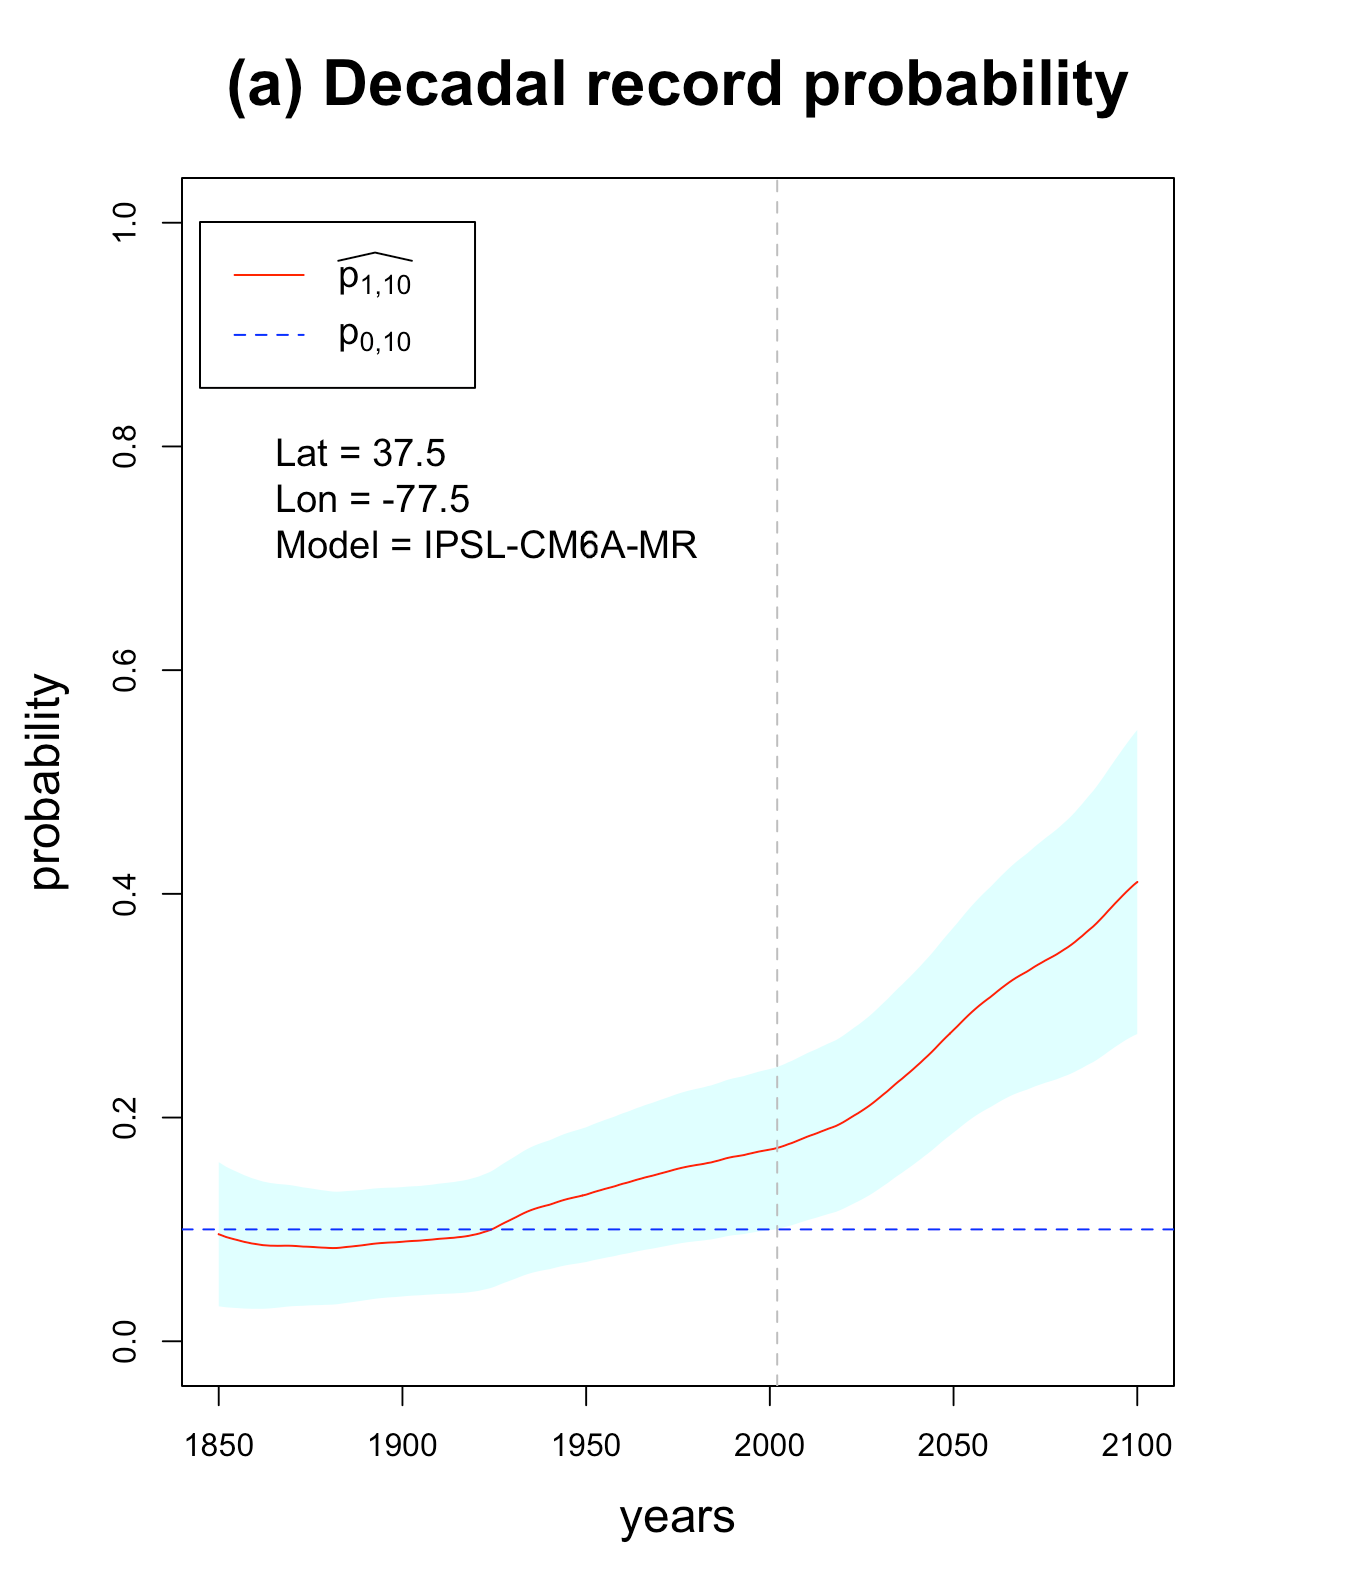
\includegraphics[width=1\textwidth]{/Users/pgonzale/Downloads/fig3_reviewed_article1_test_a.png}
 \end{center}  
 \end{column}
 \pause
 \begin{column}{0.5\textwidth}
\begin{center}
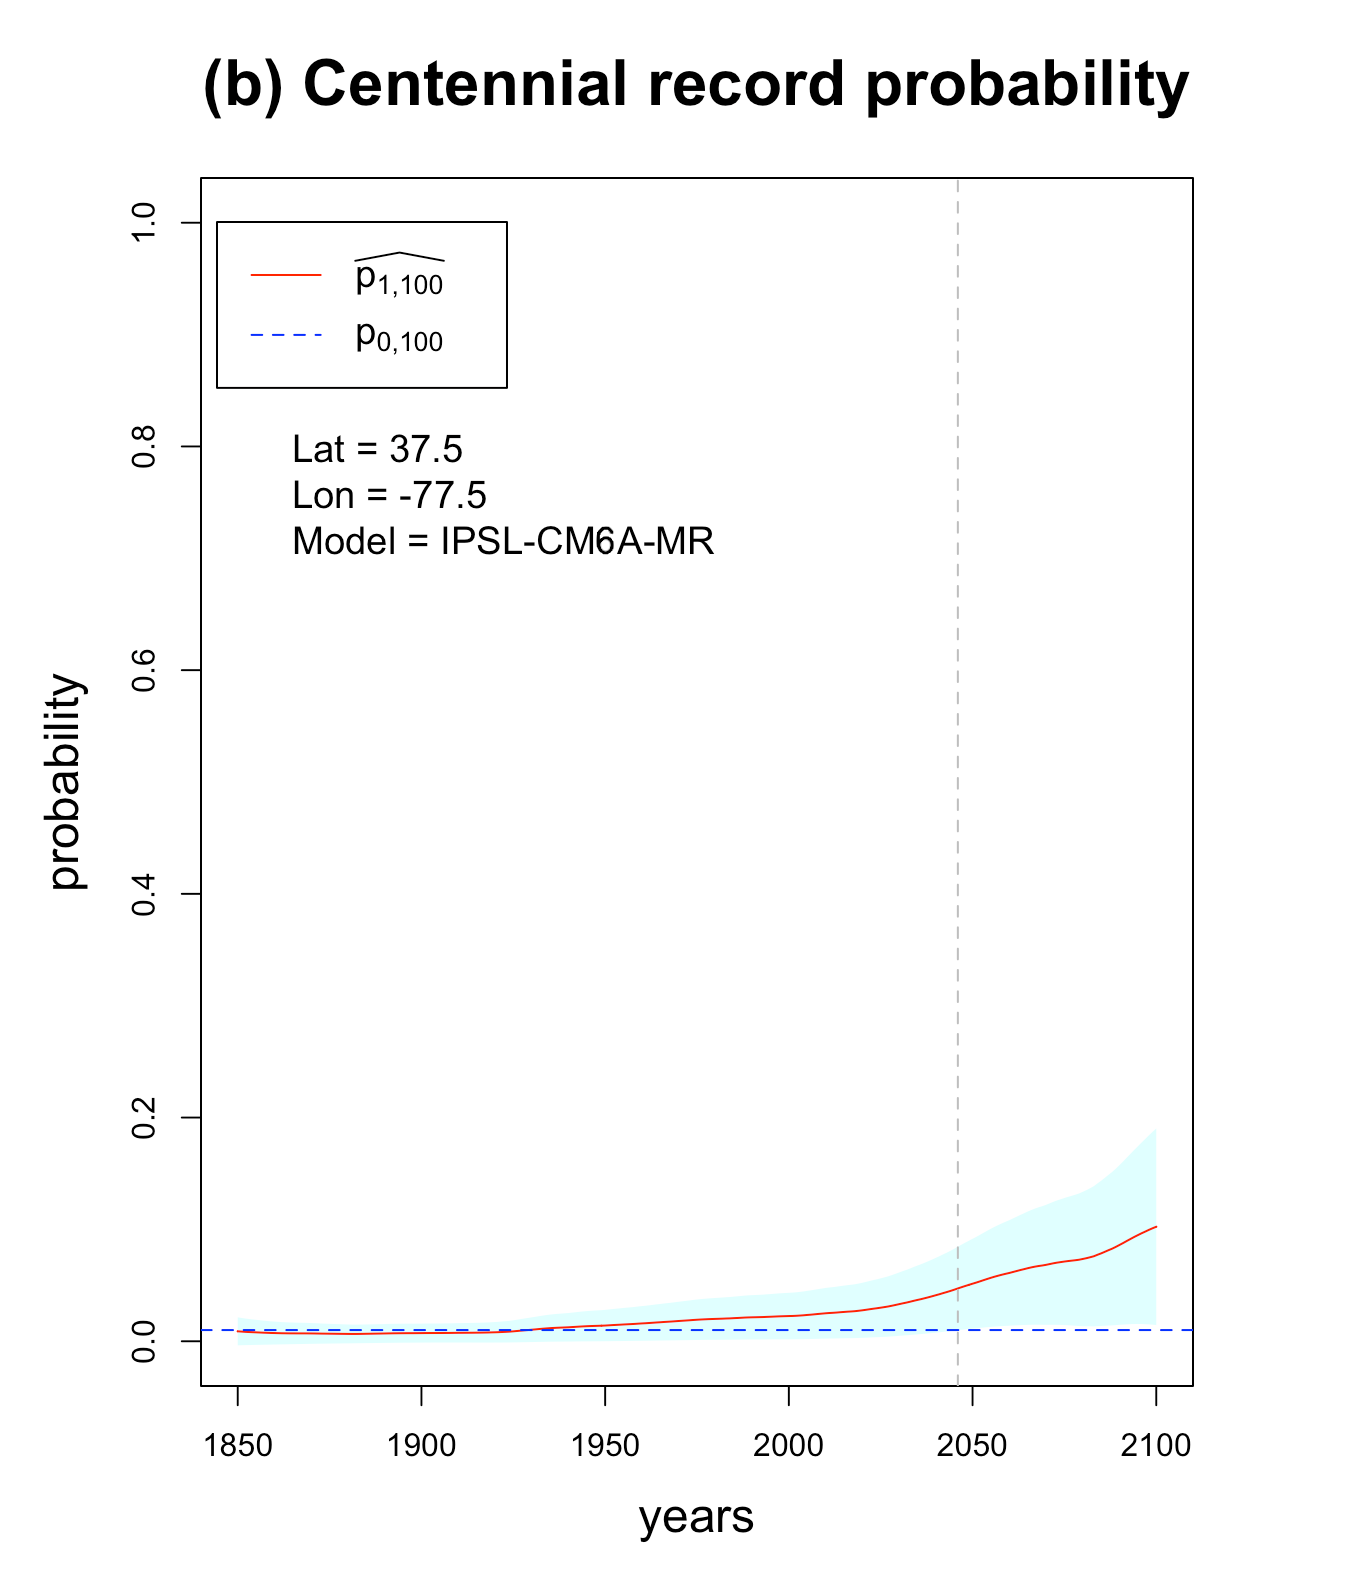
\includegraphics[width=1\textwidth]{/Users/pgonzale/Downloads/fig3_reviewed_article1_test_b.png}
 \end{center}    
 \end{column}
 \end{columns}
\end{frame}
%%%%%%%%%%%%%%%%%%%%%%%%%%%%%%%%%%%%%% 
%
%
%
%%%%%%%%%%%%%%%%%%%%%%%%%%%%%%%%%%%%%%  
\begin{frame}%{Richmond, Virginia, USA}
\begin{center}
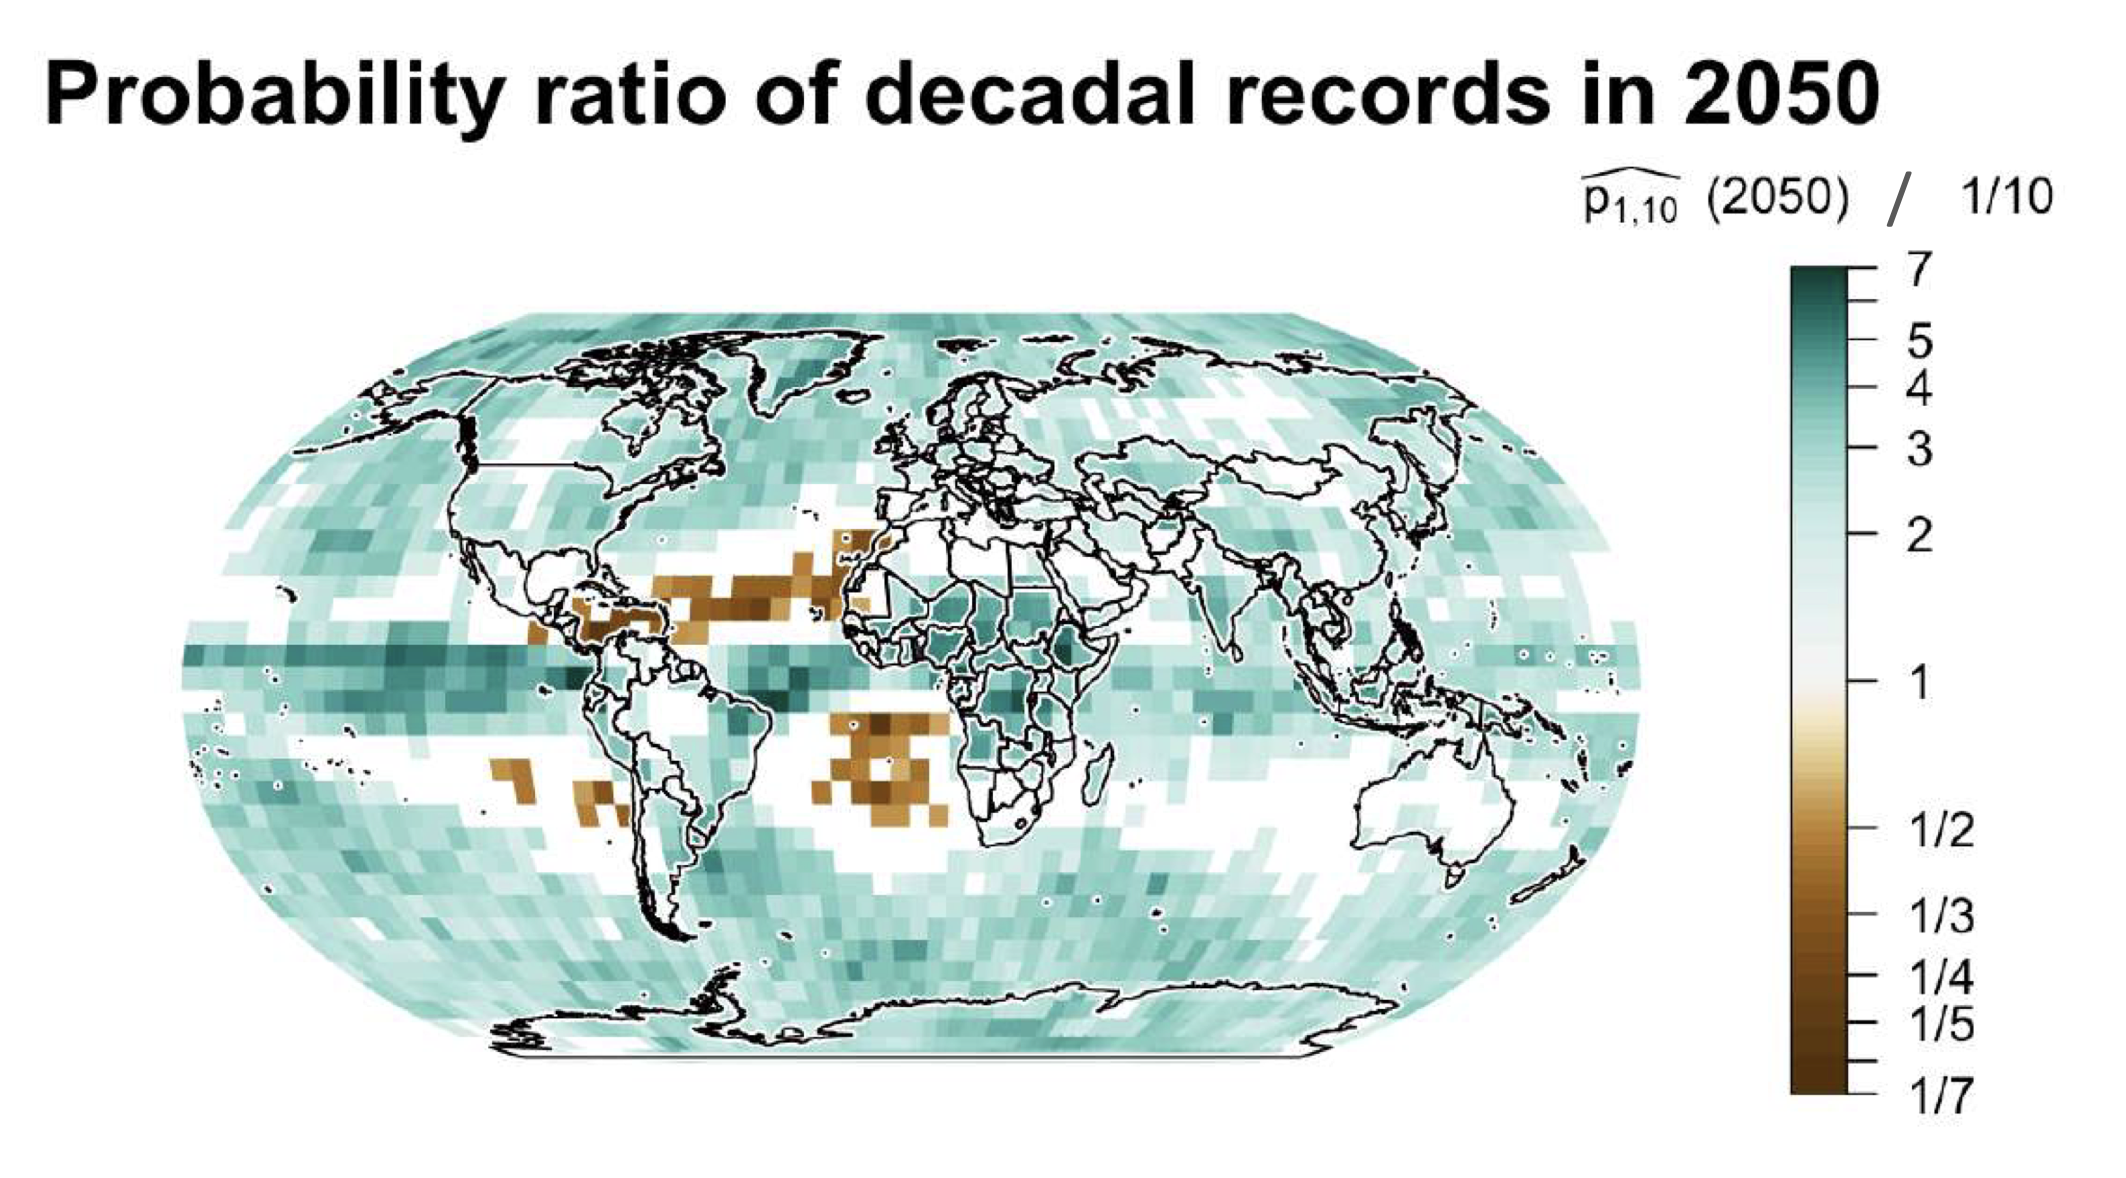
\includegraphics[width=1\textwidth]{/Users/pgonzale/Desktop/Berta/EVA2023_map1.png}
\end{center}    
\end{frame}
%%%%%%%%%%%%%%%%%%%%%%%%%%%%%%%%%%%%%% 
%
%
%
%%%%%%%%%%%%%%%%%%%%%%%%%%%%%%%%%%%%%% 
\begin{frame}%{Richmond, Virginia, USA}
\begin{center}
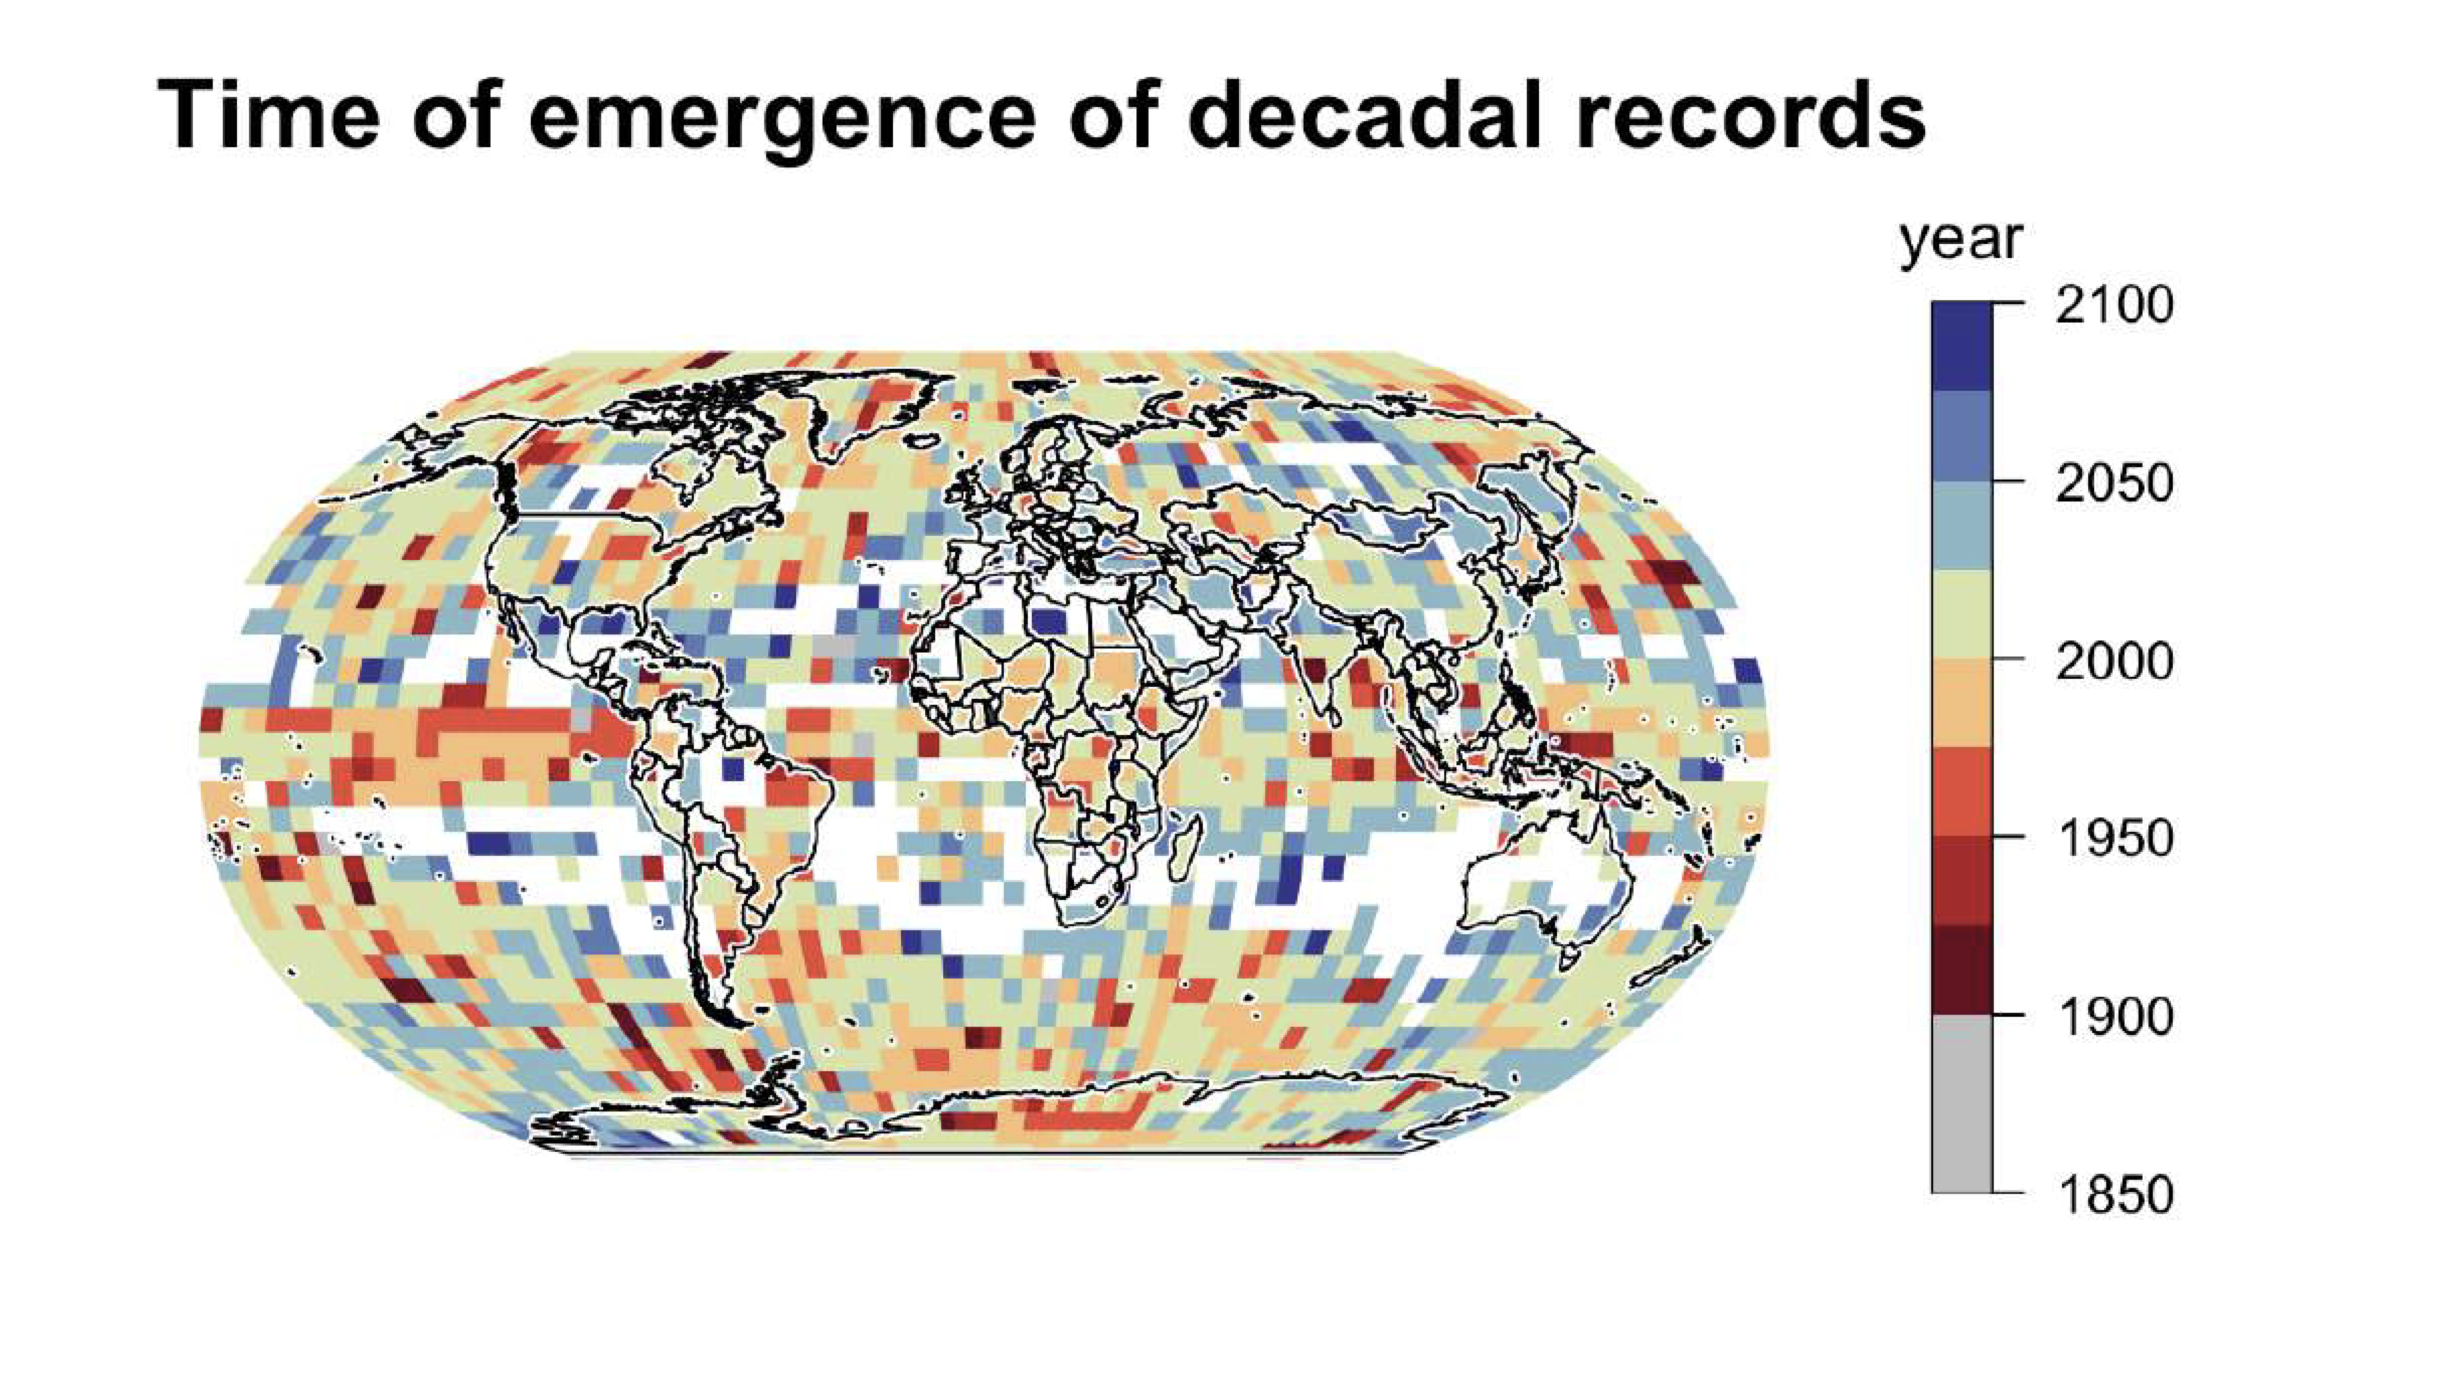
\includegraphics[width=1\textwidth]{/Users/pgonzale/Desktop/Berta/valpred2023_carte2.png}
\end{center}    
\end{frame}
%%%%%%%%%%%%%%%%%%%%%%%%%%%%%%%%%%%%%% 
%
%
%
%%%%%%%%%%%%%%%%%%%%%%%%%%%%%%%%%%%%%%  
\begin{frame}{Summary of part 1}
\begin{block}{Noticeable statistical  features}
 \begin{itemize}
	\item {\bf Transient EEA of records}
	\item Bypassing the estimation of the GEV parameters
	\item Only 2 parameters need to be estimated
	\item Allow different tail parameters $\xi$ in marginals
	\item Kernel smoothing Method-of moments full captures non-linear trends
\end{itemize}
\end{block} 
\vfill
\begin{block}{Climatological  records}
 \begin{itemize}
	\item  Precipitation records are affected all over the world
	\item  Consistent with previous studies on changes of precipitation.
\end{itemize}
\end{block} 

\end{frame}

%%%%%%%%%%%%%%%%%%%%%%%%%%%%%%%%%%%%%%  
%
%
%
\setbeamercolor{section in head/foot}{bg=red@schema}
\setbeamercolor{subsection in head/foot}{bg=red@schema}
%%%%%%%%%%%%%%%%%%%%%%%%%%%%%%%%%%%%%% 
\section{Part 2}
{\setbeamercolor{background canvas}{bg=red@schema}
\begin{frame}
\begin{center}
\textbf{\LARGE {\color{beamer@blendedblue} Forecasting yearly record probabilities \\
from historical measurements}}
 \bigskip
 \bigskip

\LARGE {\color{beamer@blendedblue} (Part 2)}
\end{center}
 \bigskip
 \bigskip
 \bigskip
 \bigskip
 
{\tiny
\begin{myboxred}
Shortly deposited on HAL (Gonzalez et al., 2025).
\end{myboxred}
}


\end{frame}
}
%%%%%%%%%%%%%%%%%%%%%%%%%%%%%%%%%%%%%%  
%
%
%
%%%%%%%%%%%%%%%%%%%%%%%%%%%%%%%%%%%%%%
\begin{frame}{Records in Paris over a region}
\begin{center}
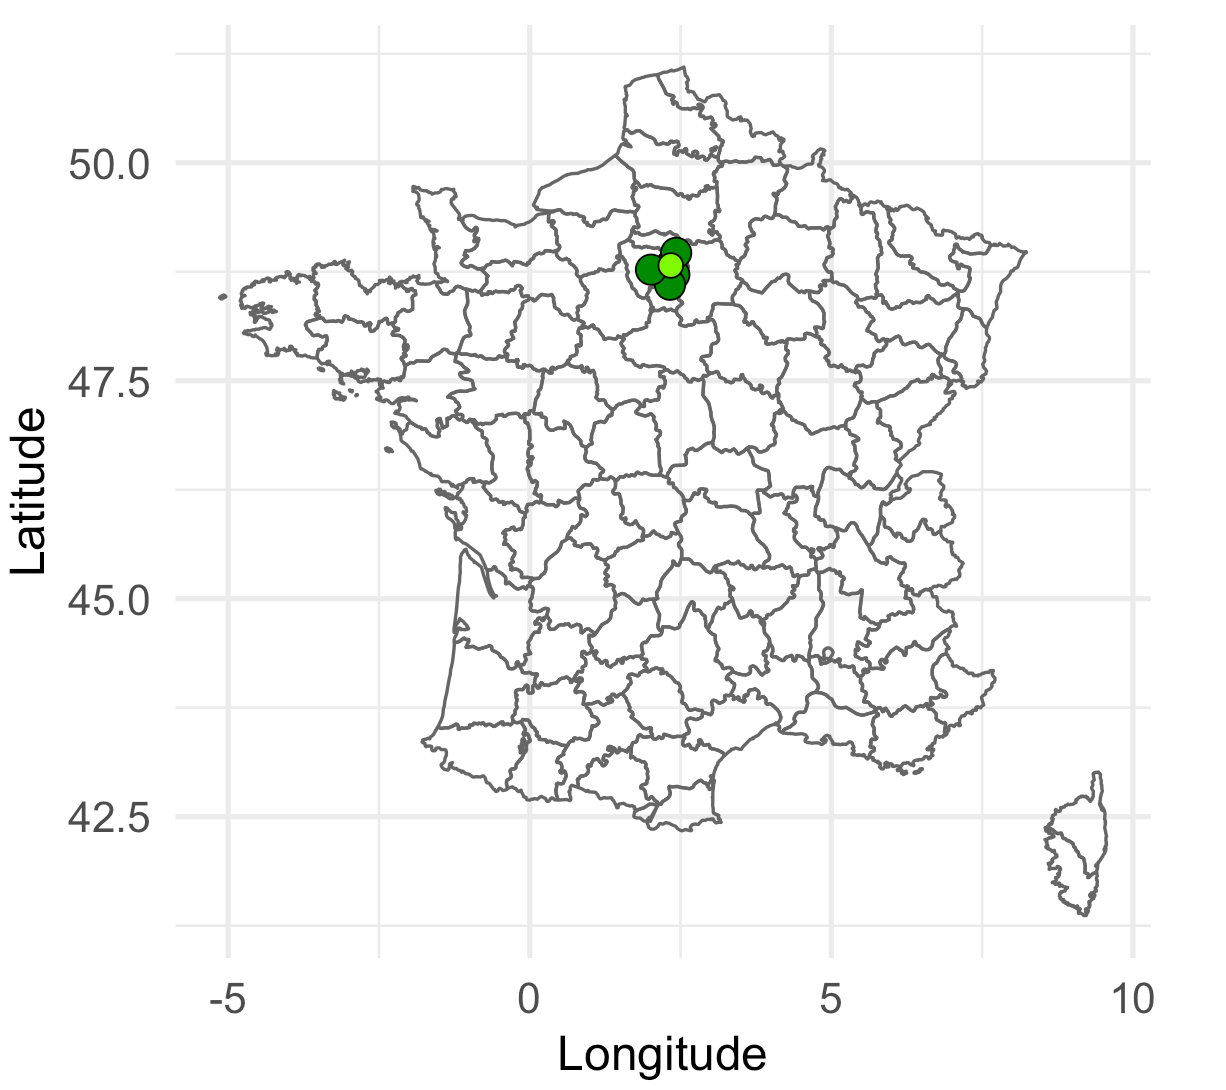
\includegraphics[width=0.75\textwidth]{/Users/pgonzale/Desktop/paris_region_map_slides.png}
 \end{center}    
\end{frame}
%%%%%%%%%%%%%%%%%%%%%%%%%%%%%%%%%%%%%% 
%
%
%
%%%%%%%%%%%%%%%%%%%%%%%%%%%%%%%%%%%%%%%
\begin{frame}{Definition of the event of study}   
\begin{tcolorbox}[title= Local records over a given region ]
$$
%P_{T+1}(s_o) =P
 \left\{  Y_{T+1}(s_o)  > \max_{s \in \mathbb{S}} \max_{t=1, \dots, T} Y_t(s)\right\}
$$
\end{tcolorbox}
\pause
\begin{tcolorbox}[title= Notation ]
$$\mathbb{S} \text{: ensemble of sites}$$
$$s_o \text{: site of interest}$$
$$T \text{: extent of the reference period}$$
$$Y_t(s) \text{: R.V associated to time time } t \text{ and site } s$$ 
\end{tcolorbox}
\end{frame}
%%%%%%%%%%%%%%%%%%%%%%%%%%%%%%%%%%%%%% 
%
%
%
%%%%%%%%%%%%%%%%%%%%%%%%%%%%%%%%%%%%%% 
\begin{frame}{Records in Paris over a region}
\begin{center}
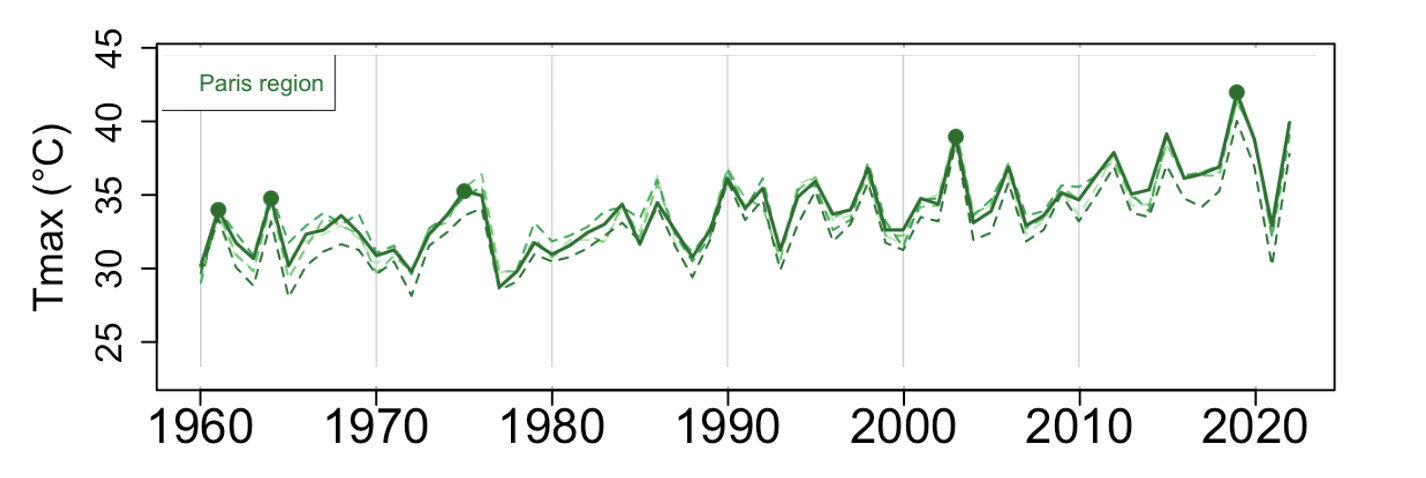
\includegraphics[scale=0.48]{/Users/pgonzale/Desktop/Berta/intro_chapter_3.png}\\
{\tiny Annual maxima of daily temperature maxima measured at {\color{red} five} stations  around Paris from 1960 to 2022}
 \end{center}    \pause
    \begin{tikzpicture}[remember picture, overlay,use page relative coordinates]
  \node[anchor=north east] at (0.81,0.9) {{\color{beamer@blendedblue}\small i) Non-linear warming trend}};
   \node[anchor=north east] at (0.775,0.85) {{\color{beamer@blendedblue}\small ii) Correlated time-series }};
    \node[anchor=north east] at (0.79,0.8) {{\color{beamer@blendedblue}\small iii) Similar range of values }};    
  \end{tikzpicture}
  
\end{frame}
%%%%%%%%%%%%%%%%%%%%%%%%%%%%%%%%%%%%%% 
%
%
%
% To study wether it is possible to identify changes in the occurence of local records, we address the following question: 
%%%%%%%%%%%%%%%%%%%%%%%%%%%%%%%%%%%%%% 
%
%
%
%%%%%%%%%%%%%%%%%%%%%%%%%%%%%%%%%%%%%%
\begin{frame}{Q2}
\begin{center}
{\LARGE{\color{beamer@blendedblue}What is the probability, at a given site, of observing a record over a given region in the upcoming year?}}
%\pause
\vfill
e.g. What is the probability of observing a record in 2023 in the center of Paris (Montsouris station) given measurement around  Paris recorded up to 2022 ?
\end{center}
\end{frame}
% What is the probability, at a given site, of observing a record over a given region in the upcoming year?
% The site of interest an it surrounding region has to be selected by the practitioner
% for example, the mayor of Paris can wonder what is the probability of observing a record in the upcoming year in the center Paris over its surrounding region.
% This translates to the following inferential objective 
%%%%%%%%%%%%%%%%%%%%%%%%%%%%%%%%%%%%%% 
%
%
%
%%%%%%%%%%%%%%%%%%%%%%%%%%%%%%%%%%%%%% 
\begin{frame}  
\begin{tcolorbox}[title= Inferential objective ]
$$
P_{T+1}(s_o) =P\left( Y_{T+1}(s_o)  \geq \max_{s \in \mathbb{S}} \max_{t=1, \dots, T} Y_t(s)\right)
$$
\end{tcolorbox}
\pause
%\begin{tcolorbox}[title= $ P_{T+1}(s_o) $ in the trivial case :  ]
%Let $Y_t(s)$ be independent identically distributed R.V for any $t=\{1,\dots,T+1\}$ and $s_o,s\in \mathbb{S} $
%$$
%P_{T+1}^{(i.i.d.)} = \frac{1}{1 + T \times S} =  \frac{1}{ \textbf{\#}\text{ of random variables being compared}}
%$$
%\end{tcolorbox}
\begin{tcolorbox}[title= Record probability for i.i.d. R.V   ]
$$
P_{T+1}^{(i.i.d.)} = \frac{1}{1 + T \times S} =  \frac{1}{ \textbf{\#}\text{ of random variables being compared}}
$$
\end{tcolorbox}
\pause
\begin{tcolorbox}[title= Literature on statistical models for record probabilities   ]
	\begin{itemize}
			\item Sparse for non-stationary times series, e.g. Ballerini and Resnick (1987), Wergen and Krug (2010)
			\item Very sparse on multivariate times series, e.g.  Godreche and Luck (2023)
			\item Very very sparse on forecasting of record probabilities in a non-linear multivariate context
\end{itemize}
\end{tcolorbox}

\end{frame}
%%%%%%%%%%%%%%%%%%%%%%%%%%%%%%%%%%%%%% 
%
%
%
%%%%%%%%%%%%%%%%%%%%%%%%%%%%%%%%%%%%%% 
\begin{frame}  
\begin{tcolorbox}[title=Inferential objective]
$$
P_{T+1}(s_o) =P\left( Y_{T+1}(s_o)  \geq \max_{s \in \mathbb{S}} \max_{t=1, \dots, T} Y_t(s)\right)
$$
\end{tcolorbox}
\begin{tcolorbox}[title= Our four  assumptions   ]
	\begin{enumerate}
			\item [$\textbf{(i)}\,\,\,\,$] All marginals of $Y_t(s)$ follow GEV distributions % for any $s\in\mathbb{S}$ and any $t \in \{1, \dots, T+1\}$
\pause 
\item  [$\textbf{(ii)}\,\,$] The region $\mathbb{S}$ is \textit{homogeneous}, i.e.  both the  tail index and the support of any $Y_t(s)$ %$(Y_t(s))_{t =1, \dots,T+1}$ 
are  constant\footnote{Location  $\mu_t(s)$ and scale $\sigma_t(s)$ parameters can vary in space and time
} in time and over $\mathbb{S}$. 

\pause
    \item [$\textbf{(iii)}$]  
    For any  $s \in \mathbb{S}$, all variables $\{Y_t(s)\}$  independent in time
\pause 
    \item [$\textbf{(iv)}$] 
The  spatial random  vector $\{Y_t(s)\}_{ s\in \mathbb{S}}$ follows  a max-stable multivariate distribution  with time-invariant dependence $V(.)$
\end{enumerate}
\end{tcolorbox}
\end{frame}
%%%%%%%%%%%%%%%%%%%%%%%%%%%%%%%%%%%%%% 
%
%
%
%%%%%%%%%%%%%%%%%%%%%%%%%%%%%%%%%%%%%%%
\begin{frame}{Statistical model for $ P_{T+1}(s_o)$}  
\begin{center}
${\color{beamer@blendedblue} P_{T+1}(s_o) =P\left( Y_{T+1}(s_o)  \geq \max_{s \in \mathbb{S}} \max_{t=1, \dots, T} Y_t(s)\right)}$
\end{center}
\begin{tcolorbox}[title= Main result  ]
Under assumptions $\textbf{(i)}$-$\textbf{(iv)}$,  
		\begin{eqnarray*} \label{eq:modelP}
			P_{T+1}(s_0)  &=& \frac{1}{1 + \sum_{t\leq T} {\color{red}V}\left({\color{blue}u_{t,T+1}(s_0,s_1)}, \ldots,  {\color{blue}u_{t,T+1}(s_0,s_S)}\right) }
			\label{eqn-mainPTs0}
		\end{eqnarray*} 
		where $ {\color{red}V}(.)$ is   the spatial max-stable  dependence function   and 
		$$
		 {\color{blue}u_{t,T+1}(s_0,s)} = \left( \frac{\sigma_{T+1}(s_0)}{\sigma_{t}(s)} \right)^{\! 1/\xi} 		$$
\end{tcolorbox}
\pause
\begin{tcolorbox}[title= Special cases  ]
If all same margins are equal in time (no warming trends),  
\begin{eqnarray*} \label{eq:Palpha}
    P_{T+1}^{{\color{beamer@blendedblue}V({\bf 1})}}  &=& 1/(1+T \times {\color{beamer@blendedblue}V({\bf 1})}), 
\end{eqnarray*}
with ${\color{beamer@blendedblue}V({\bf 1})}=S$ (the i.i.d. case)  and ${\color{beamer@blendedblue}V({\bf 1})}=1$  (the perfect dependence) 
\end{tcolorbox}
\end{frame}
%%%%%%%%%%%%%%%%%%%%%%%%%%%%%%%%%%%%%%%
%
%
%
%%%%%%%%%%%%%%%%%%%%%%%%%%%%%%%%%%%%%%%
\begin{frame}{Illustration example}
{\color{black}{\small $$ Y_t(s) \sim GEV(\mu_t = 26 + t  (2 ^{-3}) + t^2  (10^{-3}), \sigma_t, \xi = -0.2)
 \mbox{  $\& V=$ logistic($\alpha=.3$)} $$ }}
 %\centering
 %\begin{center}
\begin{columns}
\begin{column}{0.5\textwidth}
\begin{center}
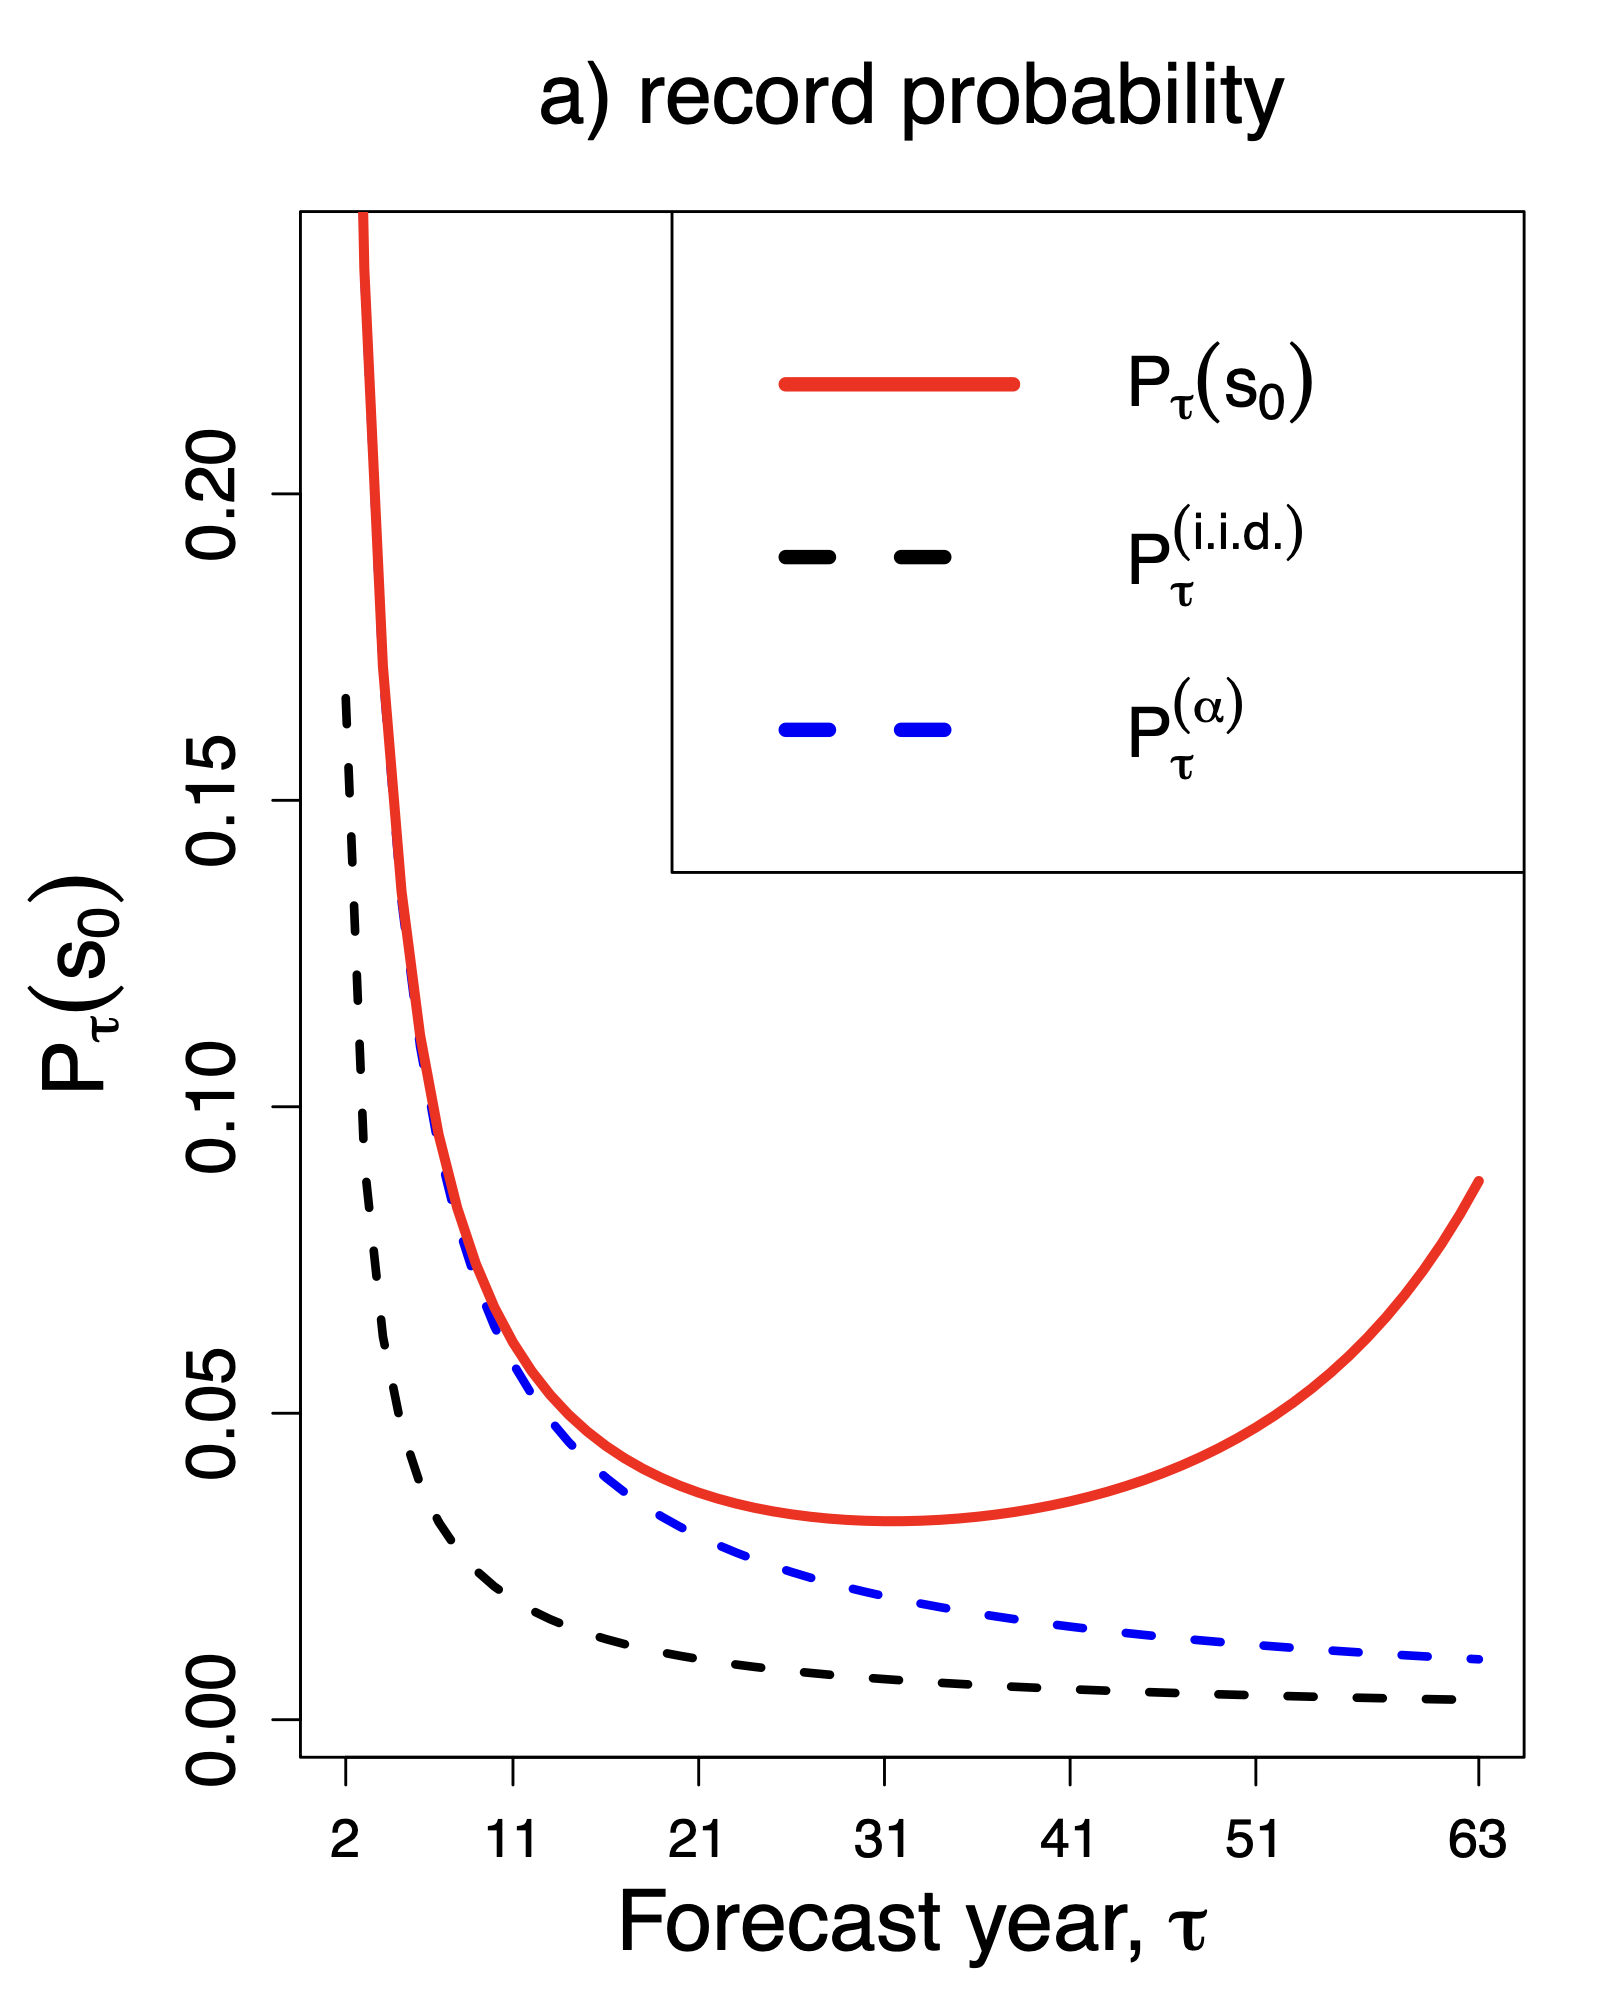
\includegraphics[width=0.9\textwidth]{/Users/pgonzale/Desktop/schemaXaida2_part1.png}
 \end{center}  
 \end{column}
 \pause
 \begin{column}{0.5\textwidth}
\begin{center}
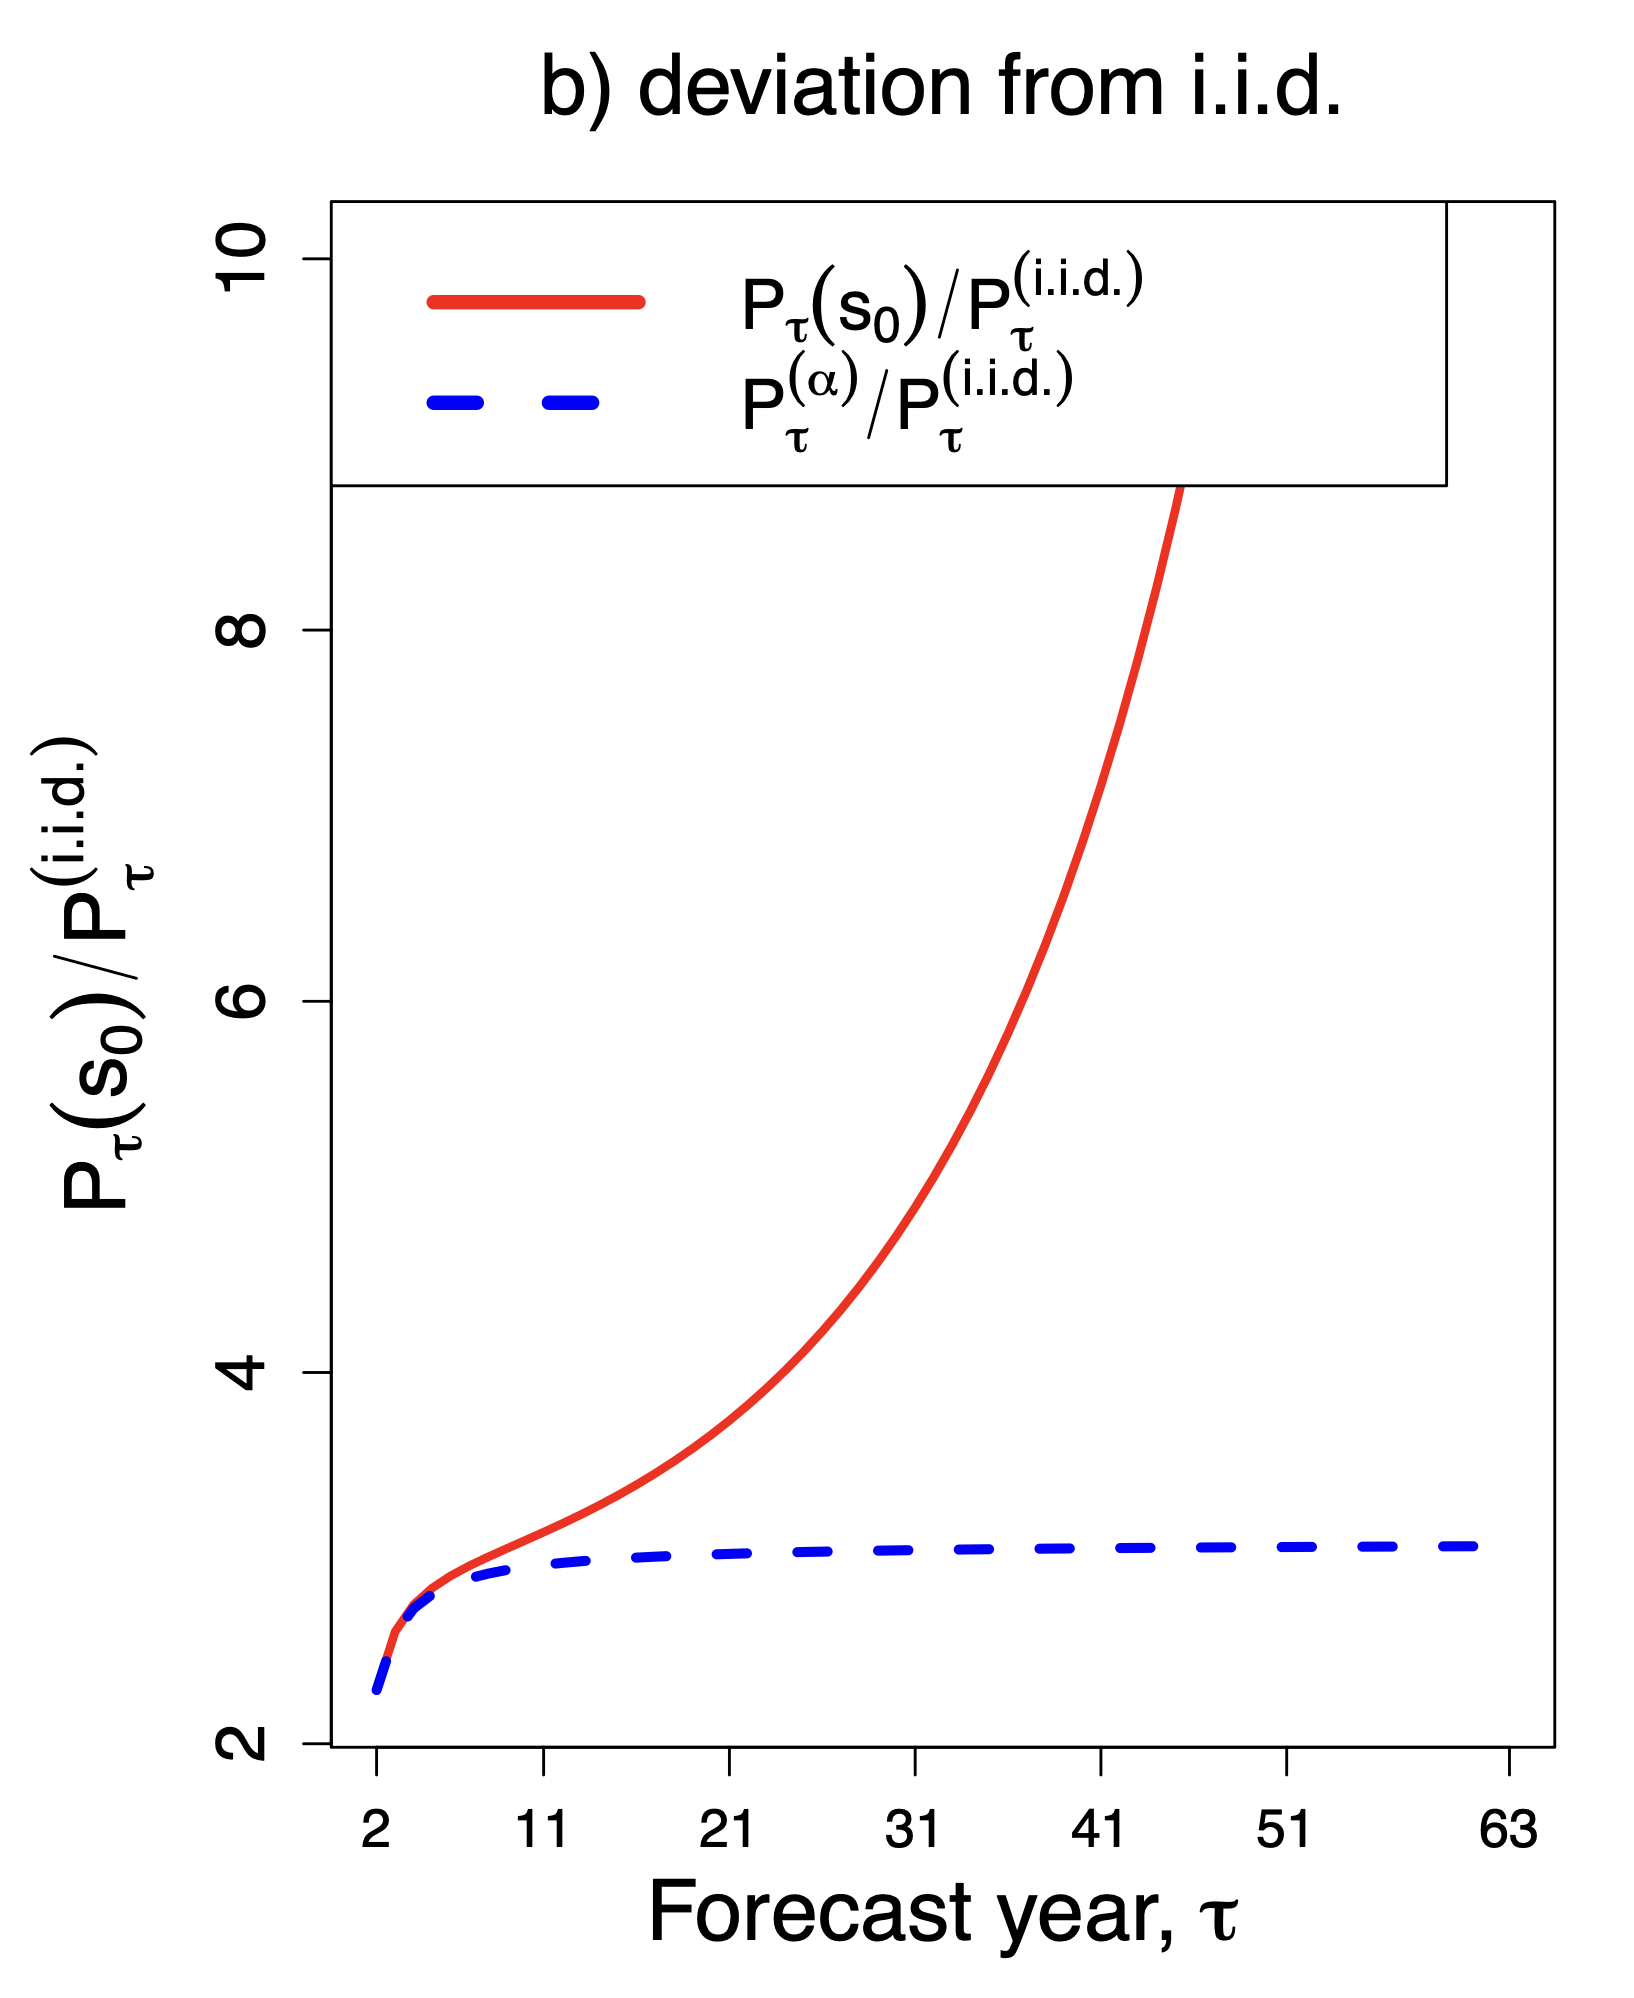
\includegraphics[width=0.9\textwidth]{/Users/pgonzale/Desktop/schemaXaida2_part2.png}
 \end{center}    
 \end{column}
 \end{columns}
 
 % \end{center}
  
 %\includegraphics[width=0.96\linewidth]{ /Users/pgonzale/schemaXaida2.pdf }
 \end{frame}
%%%%%%%%%%%%%%%%%%%%%%%%%%%%%%%%%%%%%%%
%
%
%
%%%%%%%%%%%%%%%%%%%%%%%%%%%%%%%%%%%%%%%
%
%
%
%%%%%%%%%%%%%%%%%%%%%%%%%%%%%%%%%%%%%%%
%\begin{frame}{Non-parametric Inference}  
%\begin{tcolorbox}[title= A plug-in strategy  ]
%		\begin{eqnarray*}
		%	\hat{P}_{\tau}(s_0)  &=& \frac{1}{1 + \sum_{t\leq T} {\color{red} \hat V}\left({\color{blue} \hat u}_{t,\tau}(s_0,s_1), \ldots,  {\color{blue} \hat u}_{t,%\tau}(s_0,s_S)\right) }
%		\end{eqnarray*} 
%\end{tcolorbox}

%\begin{tcolorbox}[title= A  madogram based approach (Marcon et al. 2017)  ]
%\begin{equation*}
%			 {\color{red} \hat V}({\bf x}) =  \left(\sum_{s=1}^S x^{-1}_s\right)  \times  \frac{\hat{\nu}(\textit{\textbf{w}}) + c(\textit{\textbf{w}})}{1 - \hat{\nu}(\textit{\textbf{w}}) - c(\textit{\textbf{w}})}, 
%		\end{equation*}
%		where
%		$$
%		\hat{\nu}(\textit{\textbf{w}}) = \frac{1}{T}\sum_{t=1}^{T}\left(\max_{s\in\mathbb{S}} \left\{\mathbb{F}_{t}^{(s)}(Y_{t}(s))\right\}^{1/w_s} - \frac{1}{S}\sum_{s=1}^{S} \left\{\mathbb{F}_{t}^{(s)}(Y_{t}(s))\right\}^{1/w_s} \right)
%		$$
%		and
%		$$
%		   \mathbb{F}_{t}^{(s)}(y) =\frac{1}{\sum_{k=1}^T K_{h}(t-k)}\sum_{j=1}^{T} K_{h}(t-j)1_{Y_j(s)\leq y}.
%		$$

%\end{tcolorbox}
%\end{frame}
%%%%%%%%%%%%%%%%%%%%%%%%%%%%%%%%%%%%%%%
%
%
%
%%%%%%%%%%%%%%%%%%%%%%%%%%%%%%%%%%%%%%%
%\begin{frame}{Non-parametric Inference}  
%\begin{tcolorbox}[title= A plug-in strategy  ]
%		\begin{eqnarray*}
			%\hat{P}_{\tau}(s_0)  &=& \frac{1}{1 + \sum_{t\leq T} {\color{red} \hat V}\left({\color{blue} \hat u}_{t,\tau}(s_0,s_1), \ldots,  {\color{blue} \hat u}_{t,%\tau}(s_0,s_S)\right) }
		%\end{eqnarray*} 
%\end{tcolorbox}
%\begin{tcolorbox}[title= {Method-Of-Moments as $F_t^{(s)}(Y_{\tau}(s_0)) \stackrel{d}{=}  Beta( 
    % u_{t,\tau}(s_0,s), 1)$}  ]
%\begin{equation*}
%			{\color{blue} \hat u}_{t,\tau}(s_o,s) = \frac{\widehat{E}_{t,\tau}(s_0,s)}{1 - \widehat{E}_{t,\tau}(s_0,s) }, 
%		\end{equation*}
%		with
	%	\begin{equation*}
	%		\widehat{E}_{t,\tau}(s_0,s) = \frac{1}{\sum_{l=1}^T K_{h'}(\tau-l) } \sum_{i=1}^T K_{h'}(\tau-i)\,{\mathbb{F}_{t}^{(s)}(Y_{i}(s_o))}, \mbox{ and }
	%	\end{equation*}
		%and, for every $1\leq t \leq \tau-1$,
	%	\begin{equation*}
	%		\mathbb{F}_{t}^{(s)}(y) = \frac{1}{\sum_{k=1}^T K_{h}(t-k)}\sum_{j=1}^{T} K_{h}(t-j)1_{Y_j(s)\leq y},
	%	\end{equation*}
   %
	%	\end{tcolorbox}
%\end{frame}
%%%%%%%%%%%%%%%%%%%%%%%%%%%%%%%%%%%%%%%
%
%
%
%%%%%%%%%%%%%%%%%%%%%%%%%%%%%%%%%%%%%%%
\begin{frame}{Non-parametric Inference}  

\begin{tcolorbox}[title= A plug-in strategy  ]
\textbf{(I)} For every $\tau\leq T$
		\begin{eqnarray*} \label{eq:modelP}
			\hat{P}_{\tau}(s_0)  &=& \frac{1}{1 + \sum_{t\leq T} {\color{red} \hat V}\left({\color{blue} \hat u}_{t,\tau}(s_0,s_1), \ldots,  {\color{blue} \hat u}_{t,\tau}(s_0,s_S)\right) }
\end{eqnarray*} 
\medskip
	\begin{itemize}
		\item $ {\color{red}\hat V}$ : Madogram based approach\footnotemark[10] 
		\item $ {\color{blue}\hat u_{t,\tau}(s_0,s_1)}$ : Method-Of-Moments as $F_t^{(s)}(Y_{\tau}(s_0)) \stackrel{d}{=}  Beta( {\color{blue} u_{t,\tau}(s_0,s)}, 1)$
	\end{itemize}
	\bigskip 
	\bigskip 
	
	\textbf{(II)} Forecast\footnotemark[11]  $\hat{P}_{T+1}(s_0)$ from $\{\hat{P}_{\tau}(s_0)\}_{\tau\leq T}$ \\
\end{tcolorbox}

  \footnotetext[10]{\tiny Marcon et al. (2017) }
  \footnotetext[11]{\tiny  e.g.  second order exponential smoothing, see Winters (1960), Gardner and Dannenbring (1980)}
\end{frame}

%\begin{frame}{Non-parametric Inference}  
%\begin{tcolorbox}[title= A plug-in strategy  ]
%		\begin{eqnarray*}
%			\hat{P}_{\tau}(s_0)  &=& \frac{1}{1 + \sum_{t\leq T} {\color{red} \hat V}\left({\color{blue} \hat u}_{t,\tau}(s_0,s_1), \ldots,  {\color{blue} \hat u}_{t,\tau}(s_0,s_S)\right) }
%		\end{eqnarray*} 
%\end{tcolorbox}
%\begin{tcolorbox}[title= Forecast]
%Forecasting   $\hat{P}_{T+1}(s_0)$ with a  second order 
%		exponential smoothing\footnote{Non-linear recursive extrapolation method, see Winters (1960),  Gardner \& Dannenbring (1980)}  
%\end{tcolorbox}
%\end{frame}
%%%%%%%%%%%%%%%%%%%%%%%%%%%%%%%%%%%%%%%
%
%
%
%%%%%%%%%%%%%%%%%%%%%%%%%%%%%%%%%%%%%%
\begin{frame}{Application study}
\begin{center}
\LARGE {\color{beamer@blendedblue}Yearly maxima of daily maxima temperature \\
from weather stations measurements in France}
\end{center}
\end{frame}
%%%%%%%%%%%%%%%%%%%%%%%%%%%%%%%%%%%%%%  
%
%
%
%%%%%%%%%%%%%%%%%%%%%%%%%%%%%%%%%%%%%%
\begin{frame}%{Surface temperatures records}
\begin{center}
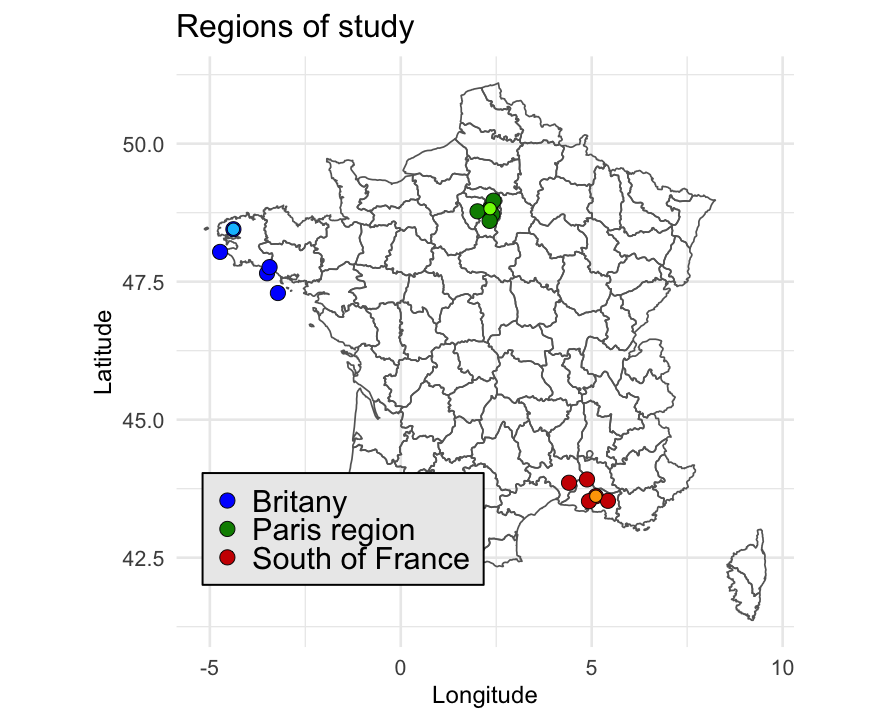
\includegraphics[width=0.9\textwidth]{/Users/pgonzale/Desktop/Berta/map2_2.png}
  \end{center}    
\end{frame}
%%%%%%%%%%%%%%%%%%%%%%%%%%%%%%%%%%%%%% 
%
%
%
%%%%%%%%%%%%%%%%%%%%%%%%%%%%%%%%%%%%%%
\begin{frame}%{Surface temperatures records}
\begin{center}
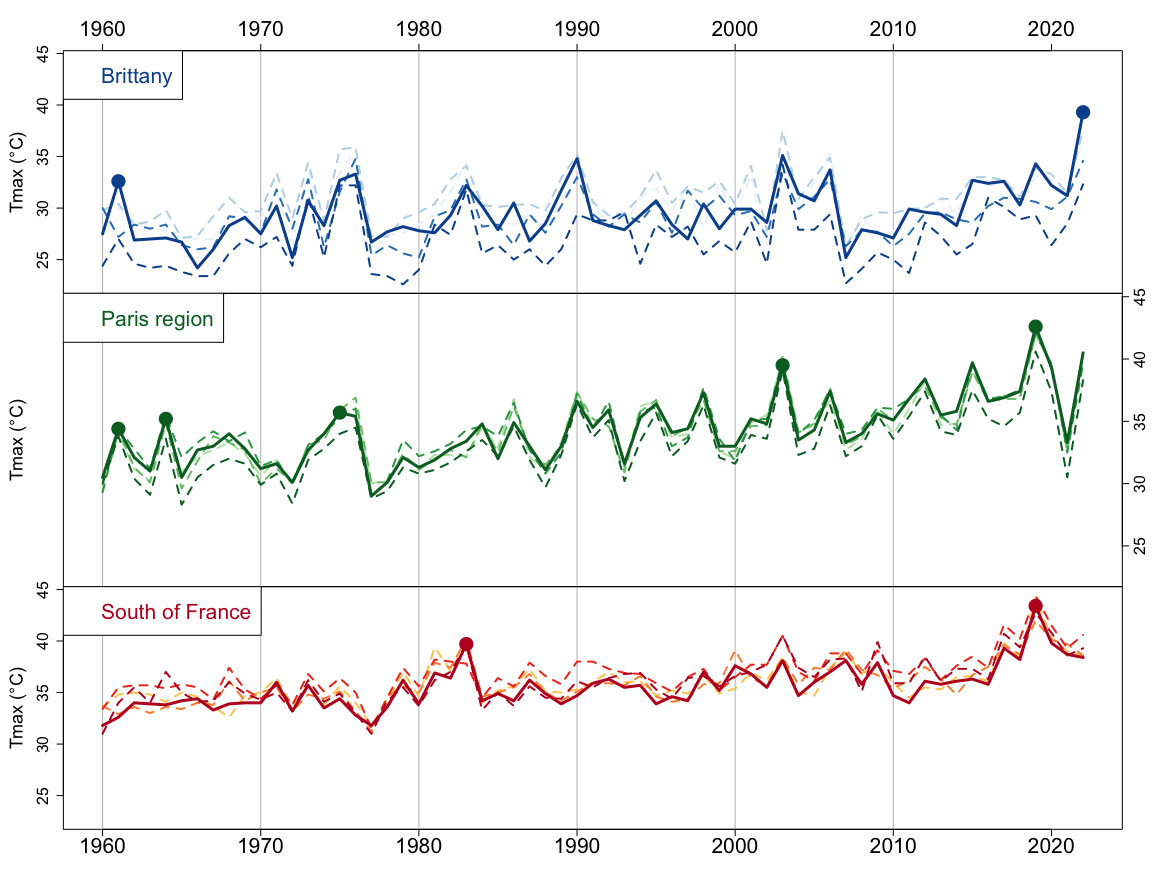
\includegraphics[width=0.94\textwidth]{/Users/pgonzale/Desktop/Berta/map1_1.png}
  \end{center}    
\end{frame}
%%%%%%%%%%%%%%%%%%%%%%%%%%%%%%%%%%%%%% 
%
%
%
%%%%%%%%%%%%%%%%%%%%%%%%%%%%%%%%%%%%%%
\begin{frame}%{Surface temperatures records}
\begin{center}
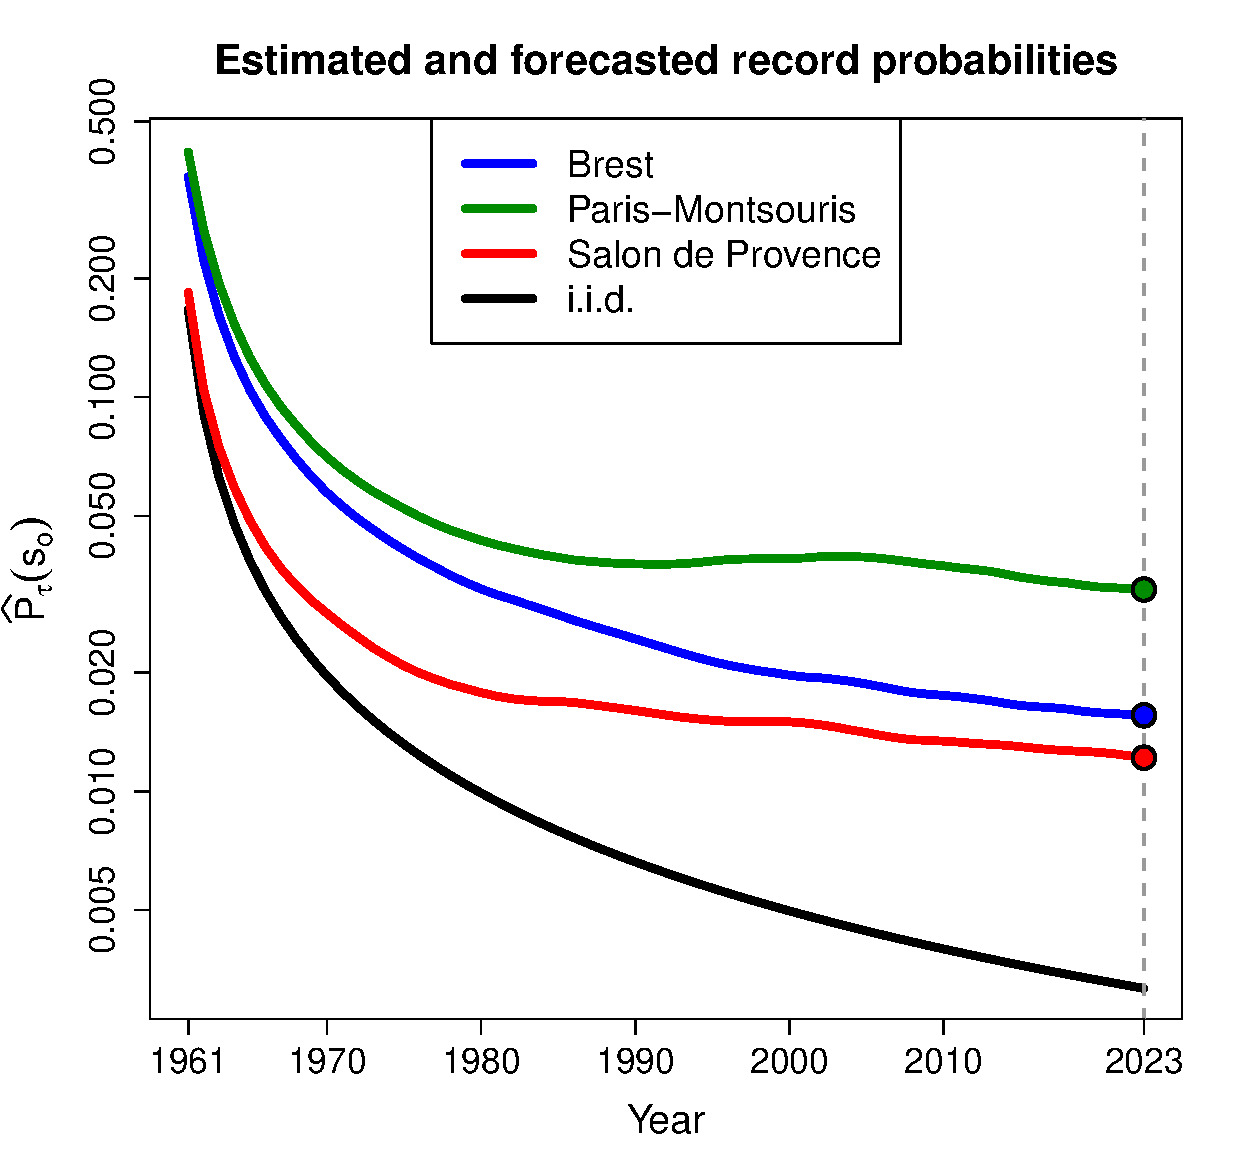
\includegraphics[width=.74\textwidth]{/Users/pgonzale/figure_Precord_part2.pdf}
  \end{center}    
\end{frame}
%%%%%%%%%%%%%%%%%%%%%%%%%%%%%%%%%%%%%%
%
%
%
%%%%%%%%%%%%%%%%%%%%%%%%%%%%%%%%%%%%%%
\begin{frame}%{Surface temperatures records}
\begin{center}
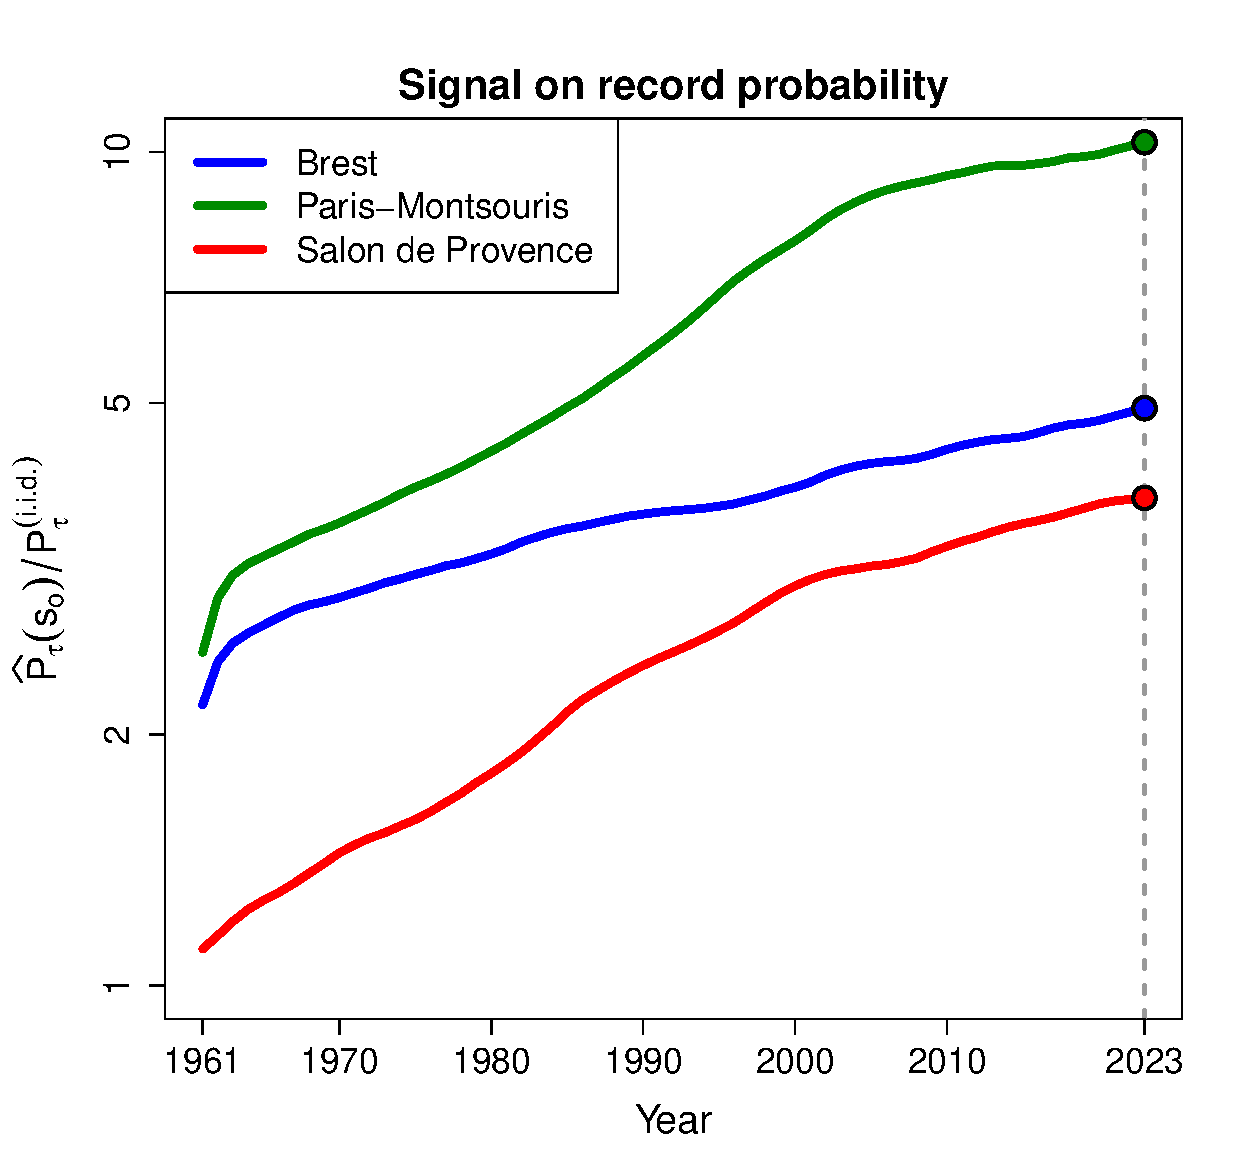
\includegraphics[width=.74\textwidth]{/Users/pgonzale/figure_Pratioiid_part2.pdf}
  \end{center}    
\end{frame}
%%%%%%%%%%%%%%%%%%%%%%%%%%%%%%%%%%%%%% 
%
%
%
%%%%%%%%%%%%%%%%%%%%%%%%%%%%%%%%%%%%%%
\begin{frame}%{Surface temperatures records}
\begin{center}
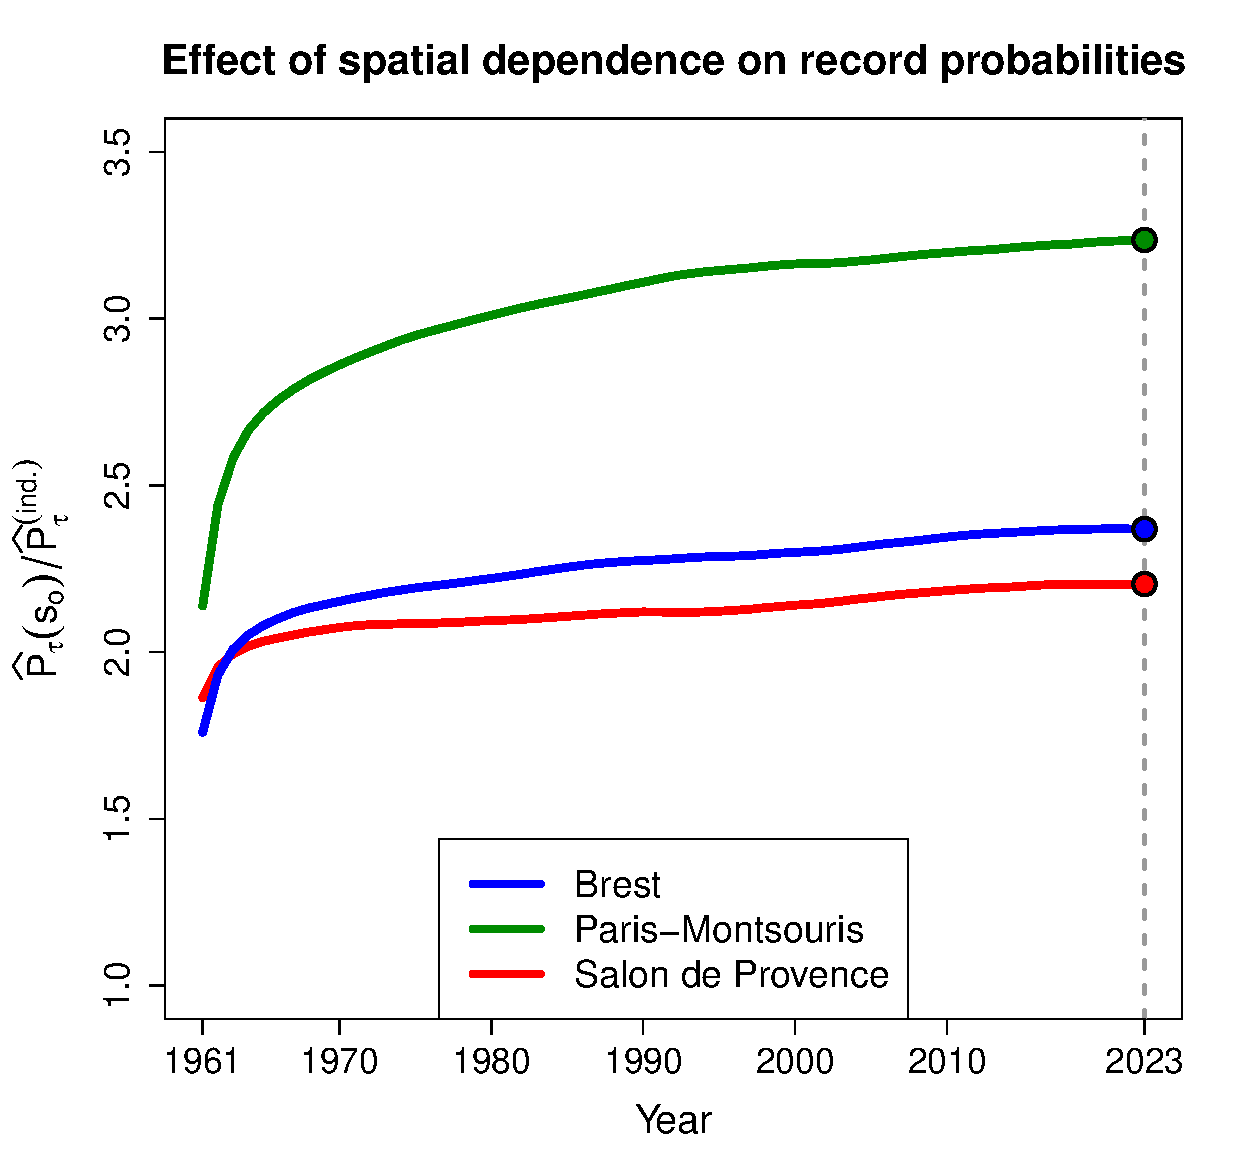
\includegraphics[width=.74\textwidth]{/Users/pgonzale/figure_Precordindep_part2.pdf}
 \end{center}    
\end{frame} 
 %%%%%%%%%%%%%%%%%%%%%%%%%%%%%%%%%%%%%%
 %
 %
 % 
 %%%%%%%%%%%%%%%%%%%%%%%%%%%%%%%%%%%%%%
\begin{frame}{Summary of part 2}
\begin{block}{Noticeable statistical  features}
 \begin{itemize}
\item {\bf Records modeling in a non-stationary and multivariate context}
\item Bypassing the estimation of the three GEV parameters 
\item Non-parametric max-stable structure
\item Fast implementations 
\end{itemize}
\end{block} 
%\pause 
\begin{block}{Climatological  records}
 \begin{itemize}
\item Inter-annual forecasting  of record probabilities seems possible 
\item  Both trends and dependence strength play a role.  % Paris regions more likely to observe a record than Brittany 
\item Negligible records under a stationary climate becomes significant (up to 8 times)
\end{itemize}
\end{block} 
\end{frame}
%%%%%%%%%%%%%%%%%%%%%%%%%%%%%%%%%%%%%%
%
%
%
 %%%%%%%%%%%%%%%%%%%%%%%%%%%%%%%%%%%%%%

%%%%%%%%%%%%%%%%%%%%%%%%%%%%%%%%%%%%%%
%
%
%
\setbeamercolor{section in head/foot}{bg=green@conclusion}
\setbeamercolor{subsection in head/foot}{bg=green@conclusion}
%%%%%%%%%%%%%%%%%%%%%%%%%%%%%%%%%%%%%%
\section{Conclusion}
{\setbeamercolor{background canvas}{bg=green@conclusion}
\begin{frame}
\begin{center}
\LARGE {\color{beamer@blendedblue} Summary of the thesis}
\end{center}
\end{frame}}
%%%%%%%%%%%%%%%%%%%%%%%%%%%%%%%%%%%%%%%
%
%
%
%%%%%%%%%%%%%%%%%%%%%%%%%%%%%%%%%%%%%%
\begin{frame}%{Surface temperatures records}
\begin{center}
%\includegraphics[width=0.75\textwidth]{/Users/pgonzale/Desktop/redandyellow_complete_slide.png}
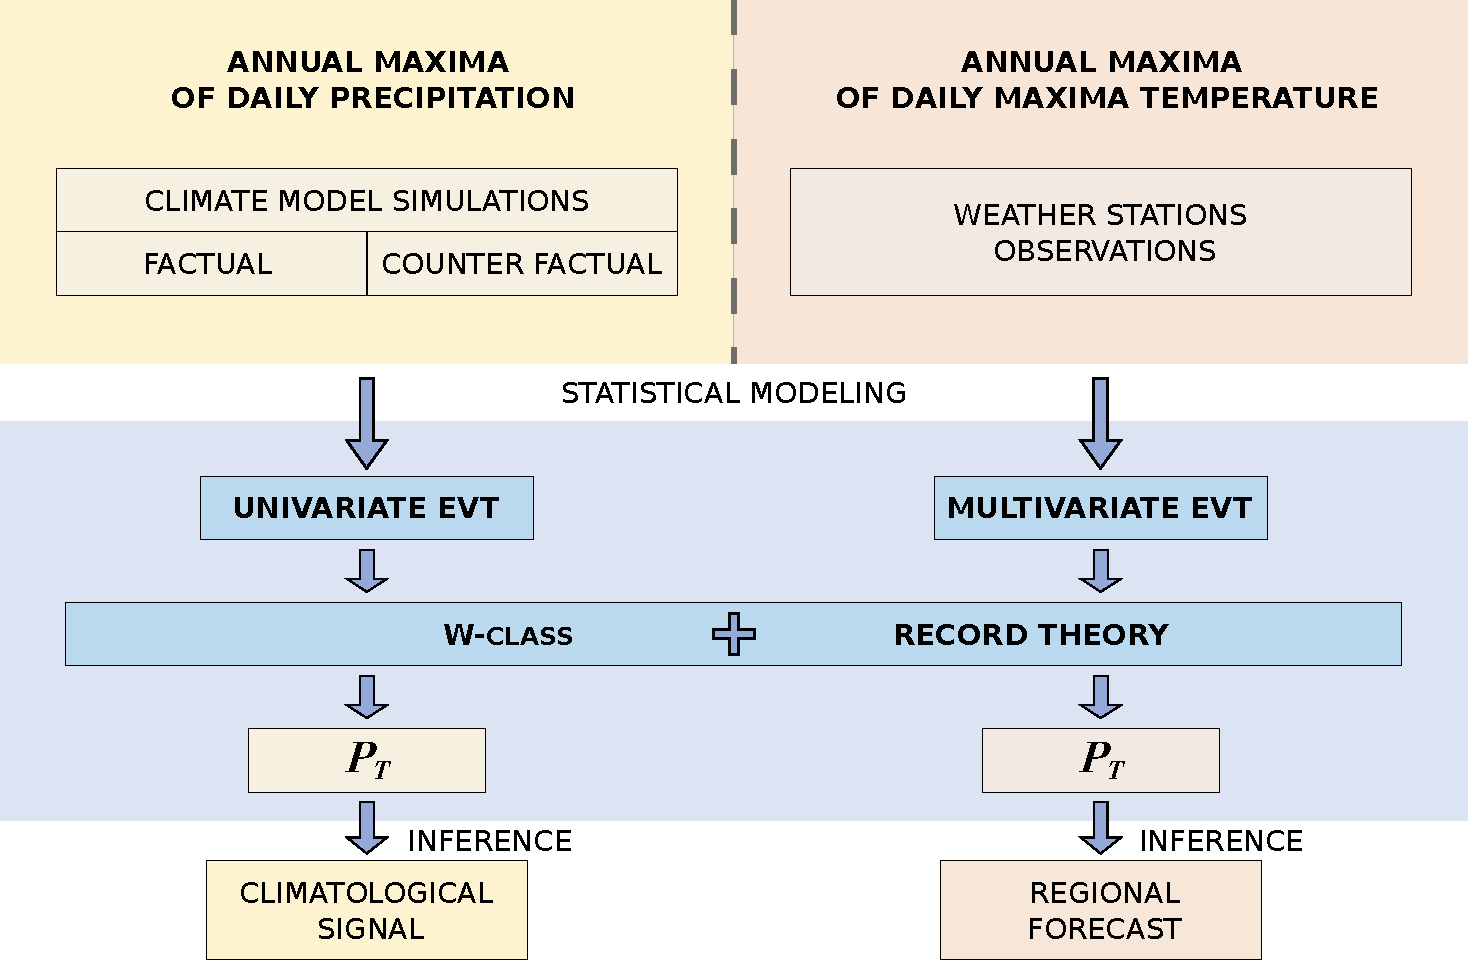
\includegraphics[width=1\textwidth]{/Users/pgonzale/Downloads/yellow_red_model.pdf}
 \end{center}    
\end{frame}
%%%%%%%%%%%%%%%%%%%%%%%%%%%%%%%%%%%%%%%
%
%
%
%%%%%%%%%%%%%%%%%%%%%%%%%%%%%%%%%%%%%%
\section{Conclusion}
\begin{frame}{Summary of the thesis}
\begin{center}
{\bf Two methodologies for the quantification of record probabilities\\ from non-stationary yearly maxima }\pause
\end{center}
\begin{block}{Global statistical features}
 \begin{itemize}
 	\item Take advantage of the relative nature of records
	\item Comprehensively account for non-linear trends
	\item Capture signals and their inter-annual changes from relatively short sample sizes
\end{itemize}
\end{block}
\pause 
\begin{block}{Limitations and perspectives ({\color{yellow@item} Q1} \&  {\color{red@item} Q2})}
 \begin{itemize}
\item No information about the magnitude of records
 \end{itemize}
\begin{columns}
\begin{column}{0.5\textwidth}
 \begin{itemize}
	\item[{\color{yellow@item}$\blacksquare$}]  Guidelines of the World Weather Attribution (WWA) protocol : 
	 \begin{itemize}
	 	\item [{\color{yellow@item}$\blacksquare$}]  Multi-model aggregation.
		\item[{\color{yellow@item}$\blacksquare$}]  Bias correction. 
		\item[{\color{yellow@item}$\blacksquare$}]  Assimilation of observations.
	 \end{itemize}
\end{itemize}
 \end{column}

 \begin{column}{0.5\textwidth}
 \begin{itemize}
	\item  [{\color{red@item}$\blacksquare$}] Uncertainty of the estimator.
	\item  [{\color{red@item}$\blacksquare$}] Move from inter-annual to multi-decadal forecast
\end{itemize} 
 \end{column}
 \end{columns}

\end{block}


\end{frame}
%%%%%%%%%%%%%%%%%%%%%%%%%%%%%%%%%%%%%%%
%
%
%
%%%%%%%%%%%%%%%%%%%%%%%%%%%%%%%%%%%%%%
{\setbeamercolor{background canvas}{bg=green@conclusion}
\begin{frame}
\begin{center}
\LARGE {\color{beamer@blendedblue} Thank you}
\end{center}
\end{frame}}
%%%%%%%%%%%%%%%%%%%%%%%%%%%%%%%%%%%%%%%
%
%
%
\setbeamercolor{section in head/foot}{bg=white}
\setbeamercolor{subsection in head/foot}{bg=white}
\section{}
%%%%%%%%%%%%%%%%%%%%%%%%%%%%%%%%%%%%%%
\appendix
\begin{frame}[noframenumbering,plain]
\begin{center}
\LARGE {\color{beamer@blendedblue} Additional material}
\end{center}
\end{frame}
%%%%%%%%%%%%%%%%%%%%%%%%%%%%%%%%%%%%%%%
%
%
%
%%%%%%%%%%%%%%%%%%%%%%%%%%%%%%%%%%%%%%
\appendix
\begin{frame}[noframenumbering,plain]{Additional material}
Part 1
\begin{itemize}
	\item Estimation algorithm for $p_{1,r}(t)$
	\item Validity of the Weibullity assumption
	\item Asymptotic confidence intervals
	\item Application on centennial records
\end{itemize}
\bigskip

Part 2
\begin{itemize}
	\item Estimation of the dependence structure $V(.)$
	\item Estimation of parameters $u_{t,\tau}(s_0,s)$
	\item Validity of the Homogeneous region assumption
\end{itemize}
\end{frame}
%%%%%%%%%%%%%%%%%%%%%%%%%%%%%%%%%%%%%%%
%
%
%
%%%%%%%%%%%%%%%%%%%%%%%%%%%%%%%%%%%%%%%
\begin{frame}[noframenumbering,plain]{Under Wclass assumption: $\,p_{1,r}(t)=\int_0^1\exp(-(r-1)\lambda_t(-\log x)^{1/k_t})\,dx$}
    
  
    
    \textbf{Estimation algorithm:}\\
    \bigskip
    
    Step 1\footnotemark[12]: $\forall \,t$\\
    
    $$ \widehat{p}_{1,2}(t)= \mathbb{E} (\mathbb{G}(Z_{t})) = \sum_{j=1}^J
    \frac{K_h(t-t_j)}{\sum_{l=1}^J K_h(t-t_l)}\mathbb{G}(Z_{t_j})$$
     
    $$\widehat{p}_{1,3}(t)= \mathbb{E} (\mathbb{G}^2(Z_{t})) =\sum_{j=1}^J
    \frac{K_h(t-t_j)}{\sum_{l=1}^J K_h(t-t_l)}\mathbb{G}^{2}(Z_{t_j})$$
    
    Step 2: for a chosen $t$
    \begin{equation*}
    \left\lbrace
    \begin{array}{l}
    \widehat{p}_{1,2}(t)=\int_0^1\exp(-\color{purple}\hat{\lambda}_t\color{black}(-\log x)^{1/\color{purple}\hat{k}_t\color{black}})\,dx\\
    \widehat{p}_{1,3}(t)=\int_0^1\exp(-2\color{purple}\hat{\lambda}_t\color{black}(-\log x)^{1/\color{purple}\hat{k}_t\color{black}})\,dx\,.
    \end{array}
    \right.\rightsquigarrow (\color{purple}\hat{k}_t\color{black},\color{purple}\hat{\lambda}_t\color{black})\end{equation*} \\
    \bigskip
    Step 3:\qquad
    ${\color{red}\widehat{p}_{1,r}(t)} \leftarrow\int_0^1\exp(-(r-1)\color{purple}\hat{\lambda}_t\color{black}(-\log x)^{1/\color{purple}\hat{k}_t\color{black}})\,dx$\\
    \footnotetext[12]{\tiny Naveau and Thao (2022)}
    \end{frame}
%%%%%%%%%%%%%%%%%%%%%%%%%%%%%%%%%%%%%%%
%
%
%
%%%%%%%%%%%%%%%%%%%%%%%%%%%%%%%%%%%%%%%
\begin{frame}[noframenumbering,plain]{Applying the transformation $T_t(w)=(w/\lambda_t)^{k_t})$ }
\begin{center}
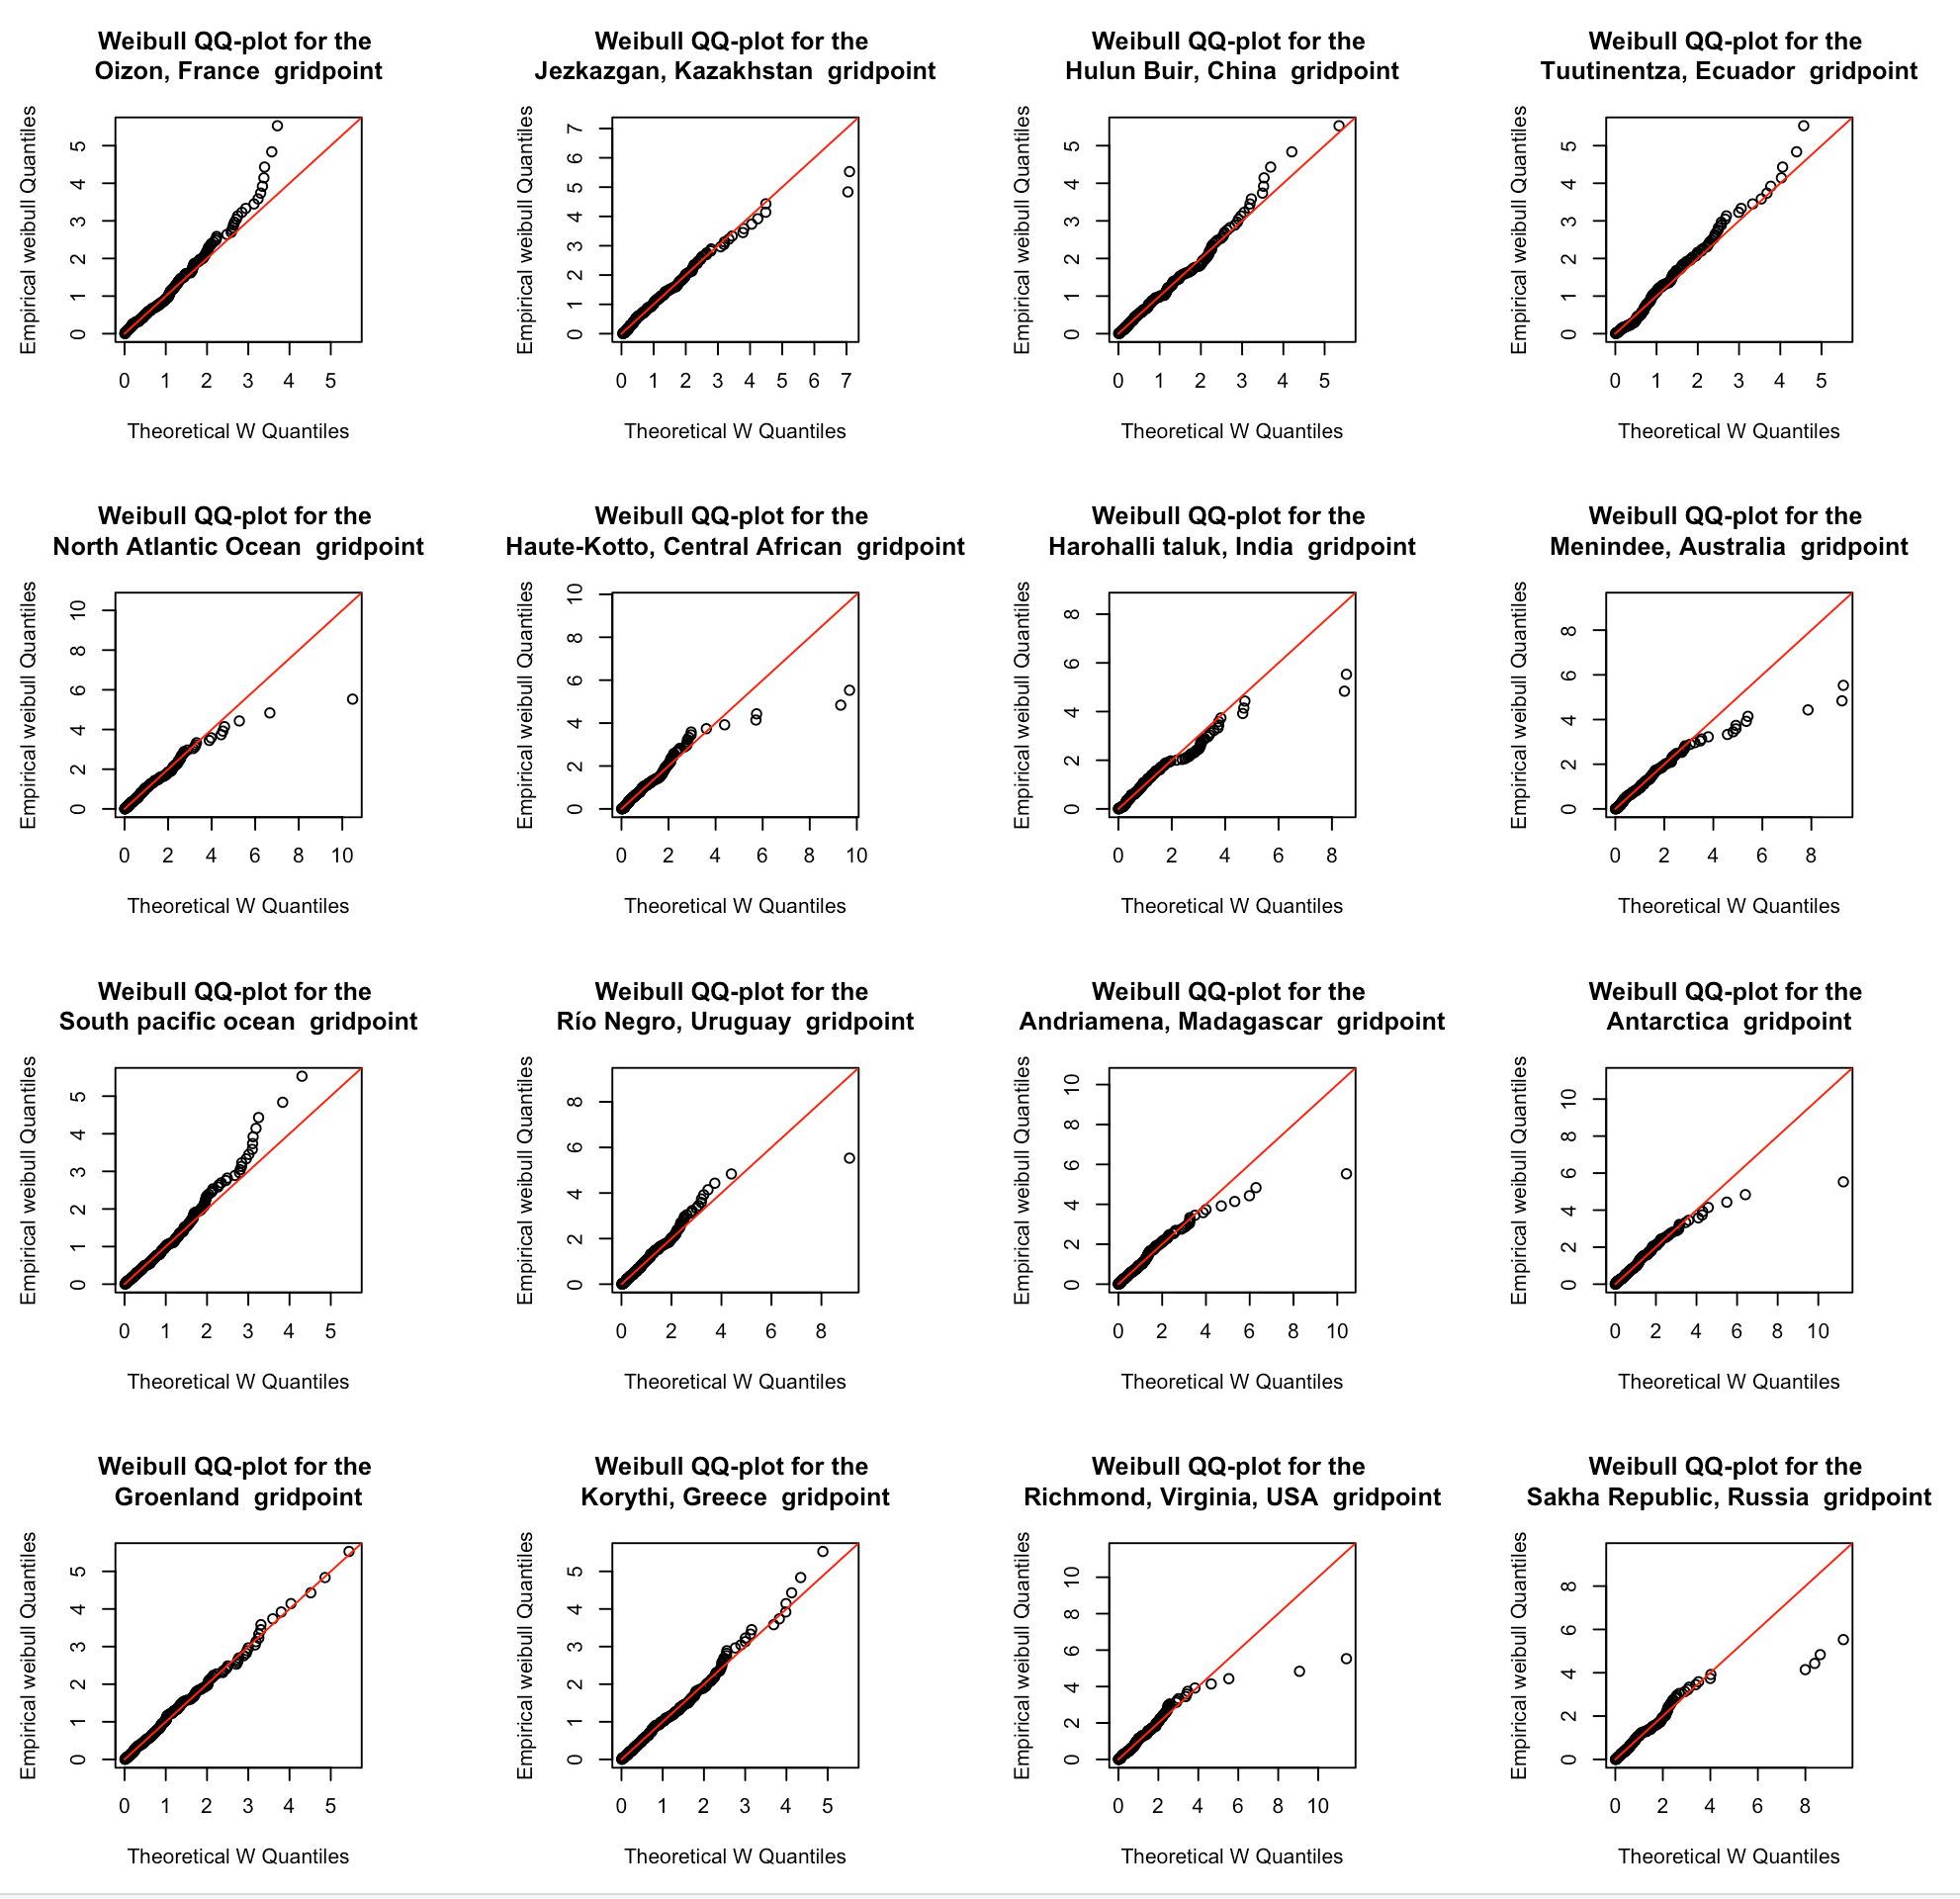
\includegraphics[width=1\textwidth]{/Users/pgonzale/Desktop/FINAL_MAI_GRL/grl_2_aout/figS1_article1.png}
 \end{center}    
 \end{frame}
%%%%%%%%%%%%%%%%%%%%%%%%%%%%%%%%%%%%%%%
%
%
%
%%%%%%%%%%%%%%%%%%%%%%%%%%%%%%%%%%%%%%%
\begin{frame}[noframenumbering,plain]{Asymptotic confidence intervals }
When  $I$ and $J$ go to infinity, if $\sqrt{J/I}$ converges to some finite constant, then for any $X_t$ and $Z_t$ belonging to the W-class and any fixed $r\geq 3$, the parametric estimator $\widehat{p}_{1,r}(t)$ satisfies
$$
\sqrt{J}\,\frac{{\color{red} \widehat{p}_{1,r}(t)}-p_{1,r}(t)}{\sigma_{rt}}\stackrel{d}{\approx}\mathcal{N}(0,1)
$$
\bigskip

Then, we can compute the confidence intervals as follows
$$
\left[{\color{red} \widehat{p}_{1,r}(t)}\pm {\color{beamer@blendedblue} z_{\alpha}\widehat{
    \sigma}_{rt}}\right]$$
with $\widehat{
    \sigma}_{rt}$ the estimation of the asymptotic standard deviation $
    \sigma_{rt}$ and $z_{\alpha}$ the significance level.
 \end{frame}
 %
%
%
%%%%%%%%%%%%%%%%%%%%%%%%%%%%%%%%%%%%%%%
\begin{frame}[noframenumbering,plain]{Asymptotic confidence intervals}
When  $I$ and $J$ go to infinity, if $\sqrt{J/I}$ converges to some finite constant, then for any $X_t$ and $Z_t$ belonging to the W-class and any fixed $r\geq 3$, the parametric estimator $\widehat{p}_{1,r}(t)$ satisfies
$$
\sqrt{J}\,\frac{{\color{red} \widehat{p}_{1,r}(t)}-p_{1,r}(t)}{\sigma_{rt}}\stackrel{d}{\approx}\mathcal{N}(0,1)
$$
with
$$
\sigma_{rt}=\sqrt{J_{r-1}(\theta_t)(J_{1,2}(\theta_t))^{-1}\Sigma_t\,(J^T_{1,2}(\theta_t))^{-1}(J_{r-1}(\theta_t))^T},
$$
\begin{itemize}
\item {\color{beamer@blendedblue} $\theta_t=(\lambda_t,k_t)$ }:  vector containing the parameters of the Weibull distribution at time $t$.
\item {\color{beamer@blendedblue} $J_i(\theta_t)$} : Jacobian matrix of {\color{beamer@blendedblue}  $g_i(\theta_t)=\int_0^1\exp(-j\lambda_t(-\log x )^{1/k_t})dx$ } at time $t$ for any integer $j\geq1$
\item  {\color{beamer@blendedblue} $J_{1,2}(\theta_t)$} : Jacobian matrix associated to {\color{beamer@blendedblue} $\theta_t\mapsto(g_1(\theta_t),g_2(\theta_t))^T$ } at time $t$.
\item {\color{beamer@blendedblue} $\Sigma_t$} : Asymptotic covariance matrix of {\color{beamer@blendedblue}  $\icol{\widehat{p}_{1,2}(t)-p_{1,2}(t) \\ \widehat{p}_{1,3}(t)-p_{1,3}(t)}$}.
\end{itemize}
 \end{frame}
%%%%%%%%%%%%%%%%%%%%%%%%%%%%%%%%%%%%%%%
%
%
%
%%%%%%%%%%%%%%%%%%%%%%%%%%%%%%%%%%%%%%%
\begin{frame}[noframenumbering,plain]%{Applying the transformation $T_t(w)=(w/\lambda_t)^{k_t})$ }
\begin{center}
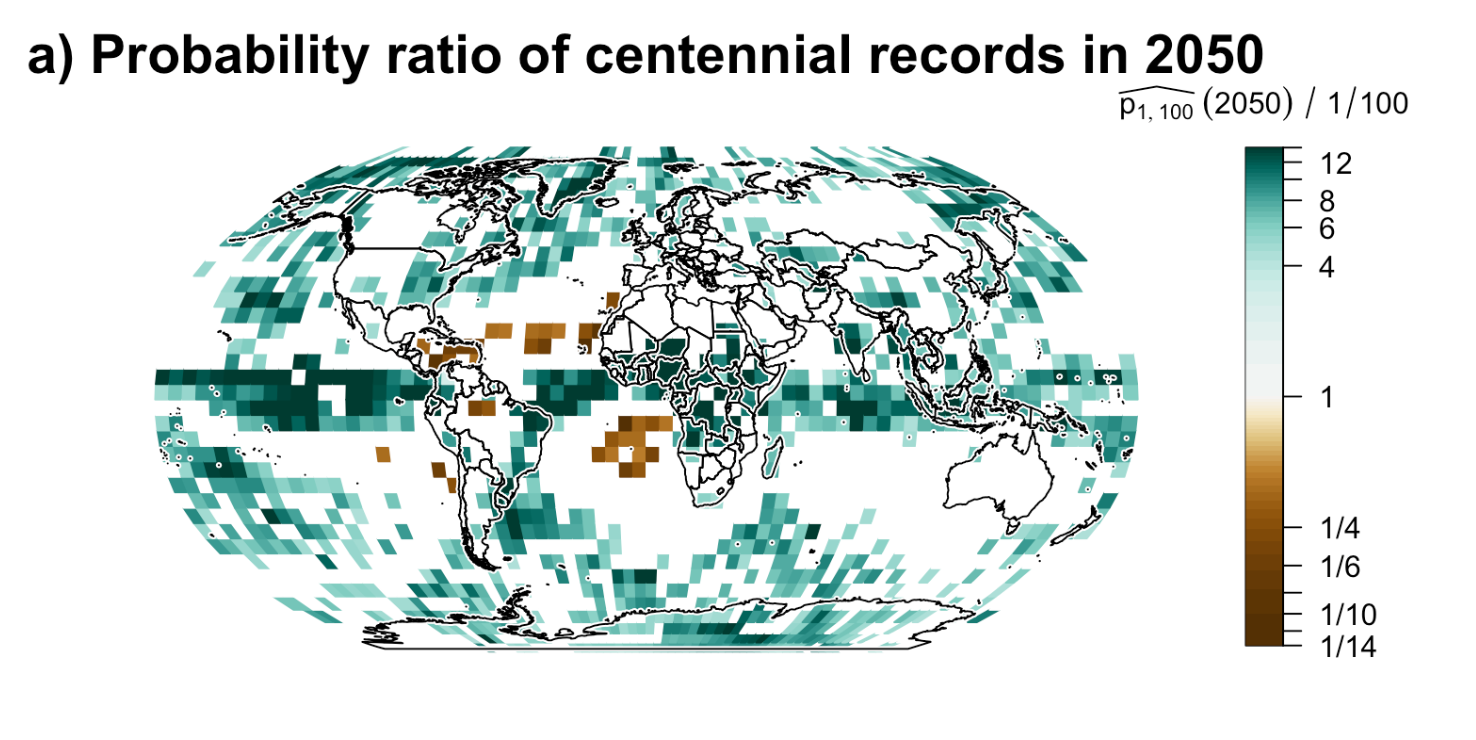
\includegraphics[width=1\textwidth]{/Users/pgonzale/Desktop/centennial_ratio_slides_soutenance.png}
 \end{center}    
 \end{frame}
%%%%%%%%%%%%%%%%%%%%%%%%%%%%%%%%%%%%%%%
%
%
%
%%%%%%%%%%%%%%%%%%%%%%%%%%%%%%%%%%%%%%%
\begin{frame}[noframenumbering,plain]%{Applying the transformation $T_t(w)=(w/\lambda_t)^{k_t})$ }
\begin{center}
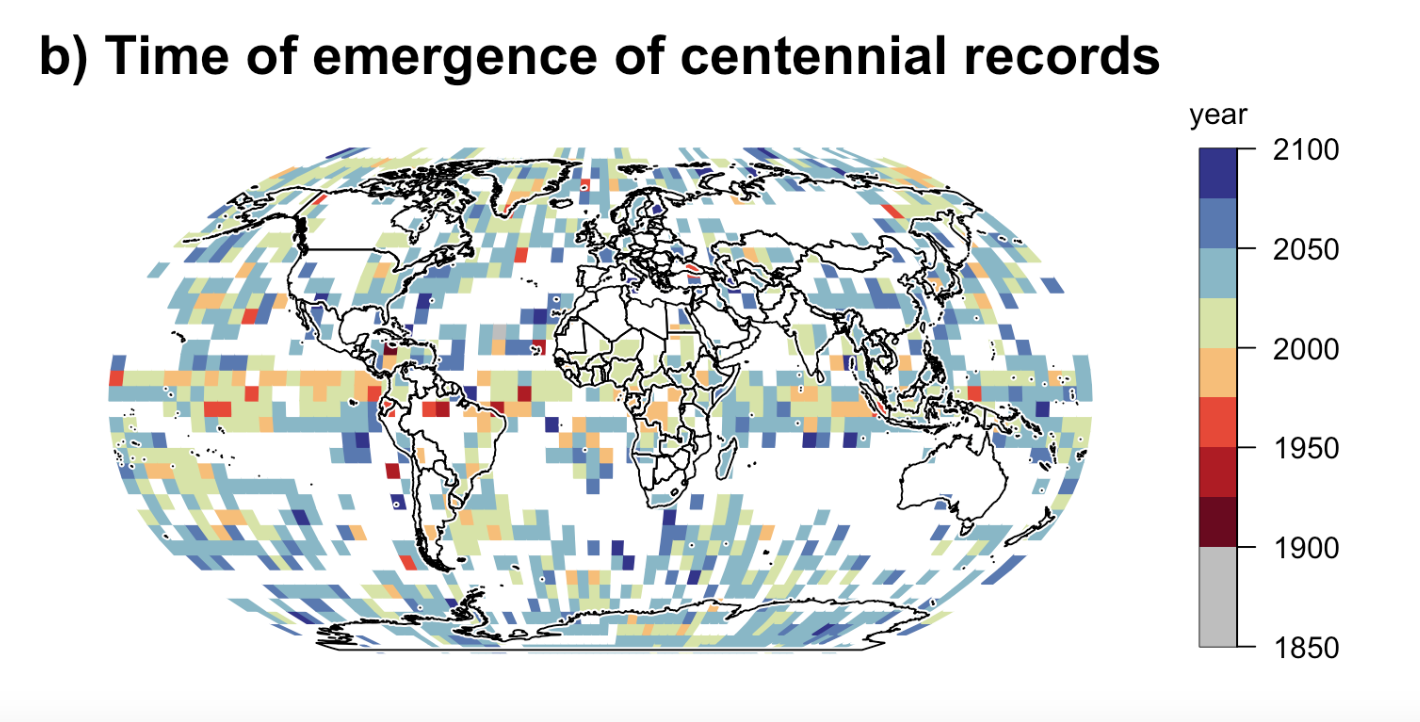
\includegraphics[width=1\textwidth]{/Users/pgonzale/Desktop/centennial_emergence_slides_soutenance.png}
 \end{center}    
 \end{frame}
%%%%%%%%%%%%%%%%%%%%%%%%%%%%%%%%%%%%%%%
%
%
%
%%%%%%%%%%%%%%%%%%%%%%%%%%%%%%%%%%%%%%%
\begin{frame}[noframenumbering,plain]{Non-parametric Inference}  
\begin{tcolorbox}[title= A  madogram based approach (Marcon et al. 2017)  ]
\begin{equation*}
			 {\color{red} \hat V}({\bf x}) =  \left(\sum_{s=1}^S x^{-1}_s\right)  \times  \frac{\hat{\nu}(\textit{\textbf{w}}) + c(\textit{\textbf{w}})}{1 - \hat{\nu}(\textit{\textbf{w}}) - c(\textit{\textbf{w}})}, 
		\end{equation*}
		with
		$$
		w_s=x_s^{-1}/\sum_{s=1}^S x^{-1}_s
		$$
		where
		$$
		\hat{\nu}(\textit{\textbf{w}}) = \frac{1}{T}\sum_{t=1}^{T}\left(\max_{s\in\mathbb{S}} \left\{\mathbb{F}_{t}^{(s)}(Y_{t}(s))\right\}^{1/w_s} - \frac{1}{S}\sum_{s=1}^{S} \left\{\mathbb{F}_{t}^{(s)}(Y_{t}(s))\right\}^{1/w_s} \right)
		$$
		$$
		c(\textit{\textbf{w}})=S^{-1}\sum_{s=1}^{S}w_s/(1+w_s)
		$$
		and
		$$
		   \mathbb{F}_{t}^{(s)}(y) =\frac{1}{\sum_{k=1}^T K_{h}(t-k)}\sum_{j=1}^{T} K_{h}(t-j)1_{Y_j(s)\leq y}.
		$$

\end{tcolorbox}
\end{frame}
%%%%%%%%%%%%%%%%%%%%%%%%%%%%%%%%%%%%%%%
%
%
%
%%%%%%%%%%%%%%%%%%%%%%%%%%%%%%%%%%%%%%%
\begin{frame}{Non-parametric Inference}  
\begin{tcolorbox}[title= A plug-in strategy  ]
		\begin{eqnarray*}
			\hat{P}_{\tau}(s_0)  &=& \frac{1}{1 + \sum_{t\leq T} {\color{red} \hat V}\left({\color{blue} \hat u}_{t,\tau}(s_0,s_1), \ldots,  {\color{blue} \hat u}_{t,\tau}(s_0,s_S)\right) }
		\end{eqnarray*} 
\end{tcolorbox}
\begin{tcolorbox}[title= {Method-Of-Moments as $F_t^{(s)}(Y_{\tau}(s_0)) \stackrel{d}{=}  Beta( 
     u_{t,\tau}(s_0,s), 1)$}  ]
\begin{equation*}
			{\color{blue} \hat u}_{t,\tau}(s_o,s) = \frac{\widehat{E}_{t,\tau}(s_0,s)}{1 - \widehat{E}_{t,\tau}(s_0,s) }, 
		\end{equation*}
		with
		\begin{equation*}
			\widehat{E}_{t,\tau}(s_0,s) = \frac{1}{\sum_{l=1}^T K_{h'}(\tau-l) } \sum_{i=1}^T K_{h'}(\tau-i)\,{\mathbb{F}_{t}^{(s)}(Y_{i}(s_o))}, \mbox{ and }
		\end{equation*}
		%and, for every $1\leq t \leq \tau-1$,
		\begin{equation*}
			\mathbb{F}_{t}^{(s)}(y) = \frac{1}{\sum_{k=1}^T K_{h}(t-k)}\sum_{j=1}^{T} K_{h}(t-j)1_{Y_j(s)\leq y},
		\end{equation*}
   
		\end{tcolorbox}
\end{frame}
%%%%%%%%%%%%%%%%%%%%%%%%%%%%%%%%%%%%%%%
%
%
%
%%%%%%%%%%%%%%%%%%%%%%%%%%%%%%%%%%%%%%
\begin{frame}[noframenumbering]%{Surface temperatures records}
\begin{center}
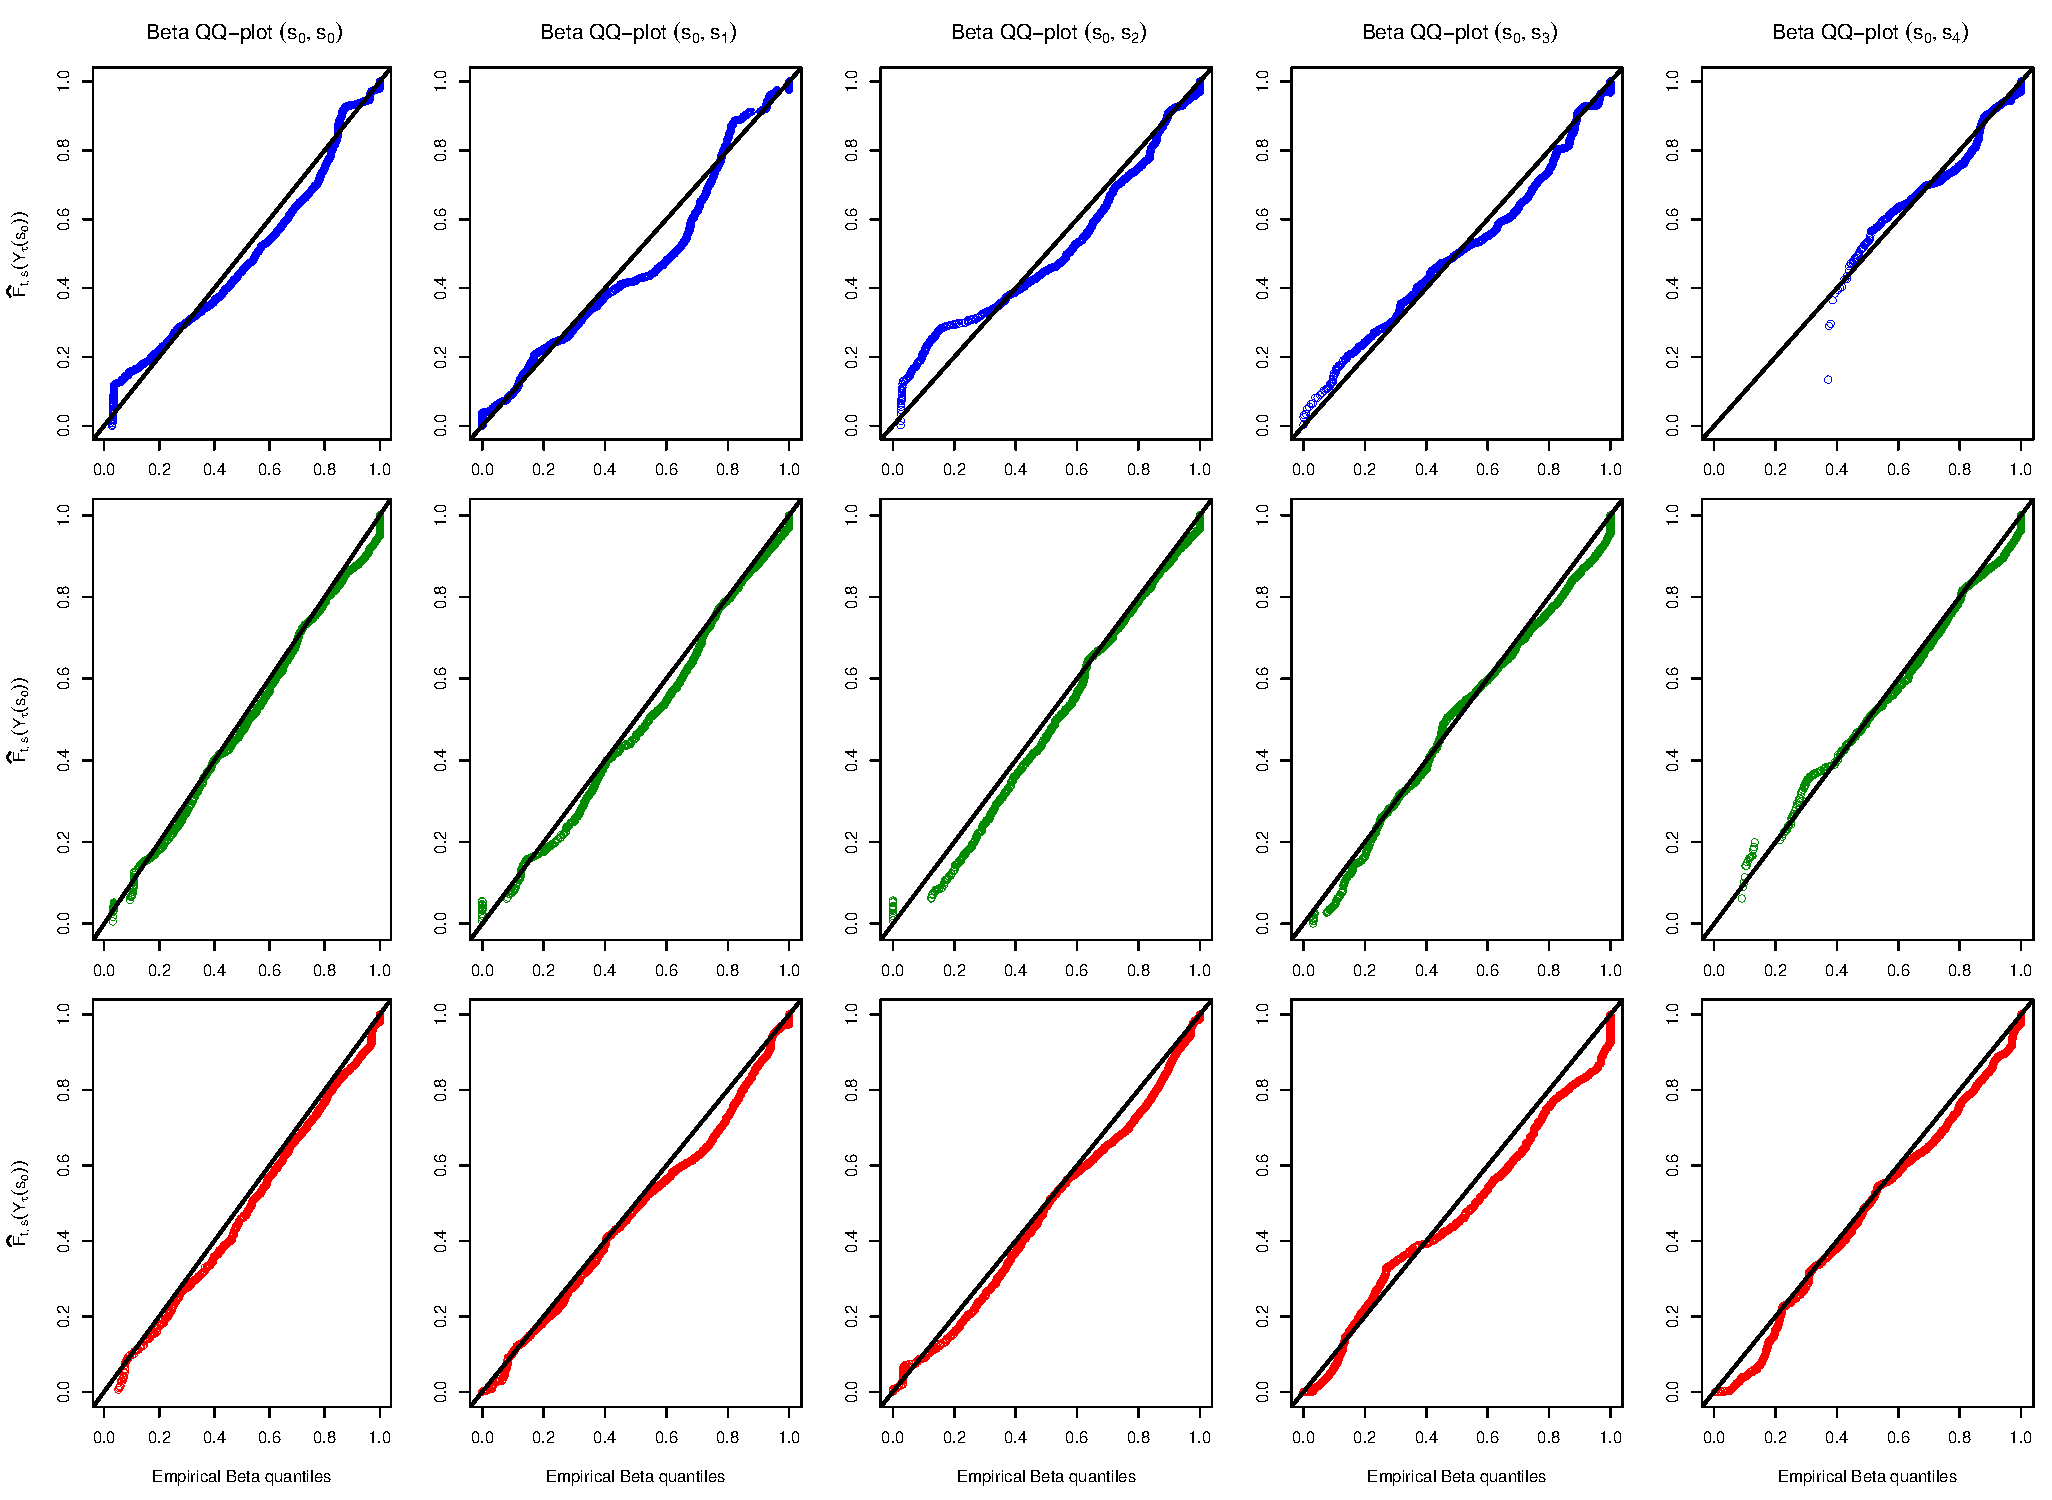
\includegraphics[width=1\textwidth]{/Users/pgonzale/QQplot_test2.pdf}
 \end{center}    
 \end{frame}
 %%%%%%%%%%%%%%%%%%%%%%%%%%%%%%%%%%%%%%
 %
%
%
\end{document} 

